\documentclass[11pt,a4paper]{article}

% Packages
\usepackage[utf8]{inputenc}
\usepackage[spanish, es-tabla]{babel}
\usepackage{amsmath}
\usepackage{amssymb}
\usepackage{upgreek}
\usepackage{accents}
\usepackage[shortlabels]{enumitem}
\usepackage{graphicx}
\usepackage{parskip}
\usepackage{tikz}		% Tener números dentro de cículos (\circled).
\usepackage{mdwlist} % Cambiar los índices en enumerate.
\usepackage{xfrac}		% Fracciones en diagonal (\sfrac).
\usepackage{lmodern} % Eliminar warning de Font shape.
\usepackage{mathtools}
\usepackage{romannum}
\usepackage{cancel}

% Definición de circled.
\newcommand*{\circled}[2][]{\tikz[baseline=(C.base)]{
	\node[inner sep=0pt] (C) {\vphantom{1g}#2};
	\node[draw, circle, inner sep=1pt, yshift=1pt]
		at (C.center) {\vphantom{1g}};}}

\begin{document}\pagenumbering{arabic}
\begin{titlepage}
\centering
\includegraphics[width=0.15\textwidth]{/Users/pedro/Desktop/DGIIM/Latex/UGR}\par\vspace{1cm}
{\scshape\LARGE Universidad de Granada \par}
\vspace{1cm}
\vspace{1.5cm}
{\huge\bfseries Álgebra II\par}
\vspace{2cm}
{\Large\itshape Pedro Ramos Suárez\par}
\vfill
Doble Grado de Ingeniería Informática y Matemáticas
\vfill
{\large \today\par}
\end{titlepage}

\tableofcontents

\newpage

\section{Combinatoria y teoría elemental de grafos}

\newpage

% 23/02/2021

\section{Grupos: definición y ejemplos}

\subsubsection*{Definición}

Un grupo $G$ es un conjunto no vacío junto con una operación interna \\ $\cdot: G \times G \to G$ satisfaciendo:
\begin{enumerate}[label=$\circled{\arabic*}$]
\item Propiedad asociativa: 
$$(ab)c = a(bc) \hspace{0.2cm} \forall a,b,c \in G$$
Muchas veces escribiremos $abc := (ab)c = a(bc)$.
\item Existencia de elemento neutro 1: 
$$1a = a1 = a \hspace{0.2cm} \forall a \in G$$ 
\item[$\circled{3}$] Existencia de inversos: 
\begin{center} $\forall a \in G \hspace{0.2cm} \exists a^{-1} \in G$ tal que $aa^{1} = 1$ \end{center}
\end{enumerate}
Si además verifica la propiedad conmutativa ($ab = ba \hspace{0.2cm} \forall a, b \in G$) entonces el grupo es abeliano o conmutativo.

\subsubsection*{Proposición}

Sea $G$ un grupo. Entonces:
\begin{enumerate}[label=$\circled{\arabic*}$]
\item En $G$ hay un único elemento neutro: la unidad o el uno de $G$.
\item Cada elemento tiene un único inverso.
\item Para cada $a \in G$, $(a^{-1})^{-1}=a$.
\item Para cualesquiera $a, b \in G$, las ecuaciones $ax= b$ y $ya = b$ tienen solución y además es única: $x = a^{-1}b$ y $y = ba^{-1}$.
\item Si $a$ es un elemento tal que $aa = 1$, entonces $a = 1$.
\item Sea $n \geq 1$ y $a_{1},...,a_{n}$. Definimos:
$$\prod_{i=1}^{1} a_{i} = a_{1}$$
$$\prod_{i=1}^{n} a_{i} = a_{n} \prod_{i=1}^{n-1}a_{i}$$
\end{enumerate}

\subsubsection*{Demostración}

\begin{enumerate}[label=$\circled{\arabic*}$]
\item Supongamos que existe otro elemento neutro $e \in G$. Entonces $1 = 1e = e$.
\item Supongamos que para $a \in G$ existe otro inverso, $a' \in G$. Entonces $a' = a'1 = a'aa^{-1} = 1a^{-1} = a^{-1}$.
\end{enumerate}

\subsubsection*{Proposición: Propiedad asociativa generalizada}

Sean $a \in G$ grupo y $n \geq 2$, entonces para cada $m$ con $1 \leq m < n$ tenemos:
$$\prod_{i=1}^{n} a_{i} = \prod_{i=1}^{m} a_{i} \prod_{i=m+1}^{n} a_{i}$$

\subsubsection*{Demostración}

El caso inicial es la propiedad asociativa. El caso general se demuestra por inducción.

\subsubsection*{Proposición}

Sea $a \in G$ grupo. Para $n \geq 1$, tenemos que:
$$(\prod_{i=1}^{n} a_{i})^{-1} = \prod_{i=1}^{n} a^{-1}_{n+i-1}$$

\subsubsection*{Demostración}

Por inducción. El caso inicial es trivial. Veamos el caso $n+1$:
$$(\prod_{i=1}^{n+1} a_{i}) (\prod_{i=1}^{n+1} a^{-1}_{n+2-i}) = (\prod_{i=1}^{n} a_{i} \cdot a_{n+1}) (a^{-1}_{n+1} \prod_{i=2}^{n+1} a_{n+2-i})= \prod_{i=1}^{n} a_{i} \prod_{i=1}^{n} a_{n+1-i} = 1$$

\subsubsection*{Definición}
Sea $a \in G$ grupo. Definimos las potencias como:
$$a^{n} = \prod_{i=1}^{n} a$$

\subsubsection*{Proposición}

Sea $G$ un grupo. Se verifican las siguientes propiedades de las potencias:
\begin{enumerate}[label=$\circled{\arabic*}$]
\item Sean $a \in G$ y $r,s > 0$. Se verifica:
$$a^{r}a^{s} = a^{r+s}$$
\item Para todo $a \in G$ y todo $n \geq 1$ se verifica:
$$(a^{n})^{-1} = (a^{-1})^{n}$$
Para cada $n \geq 1$ definimos $a^{-n}:= (a^{n})^{-1} = (a_{-1})^{n})$.
\item Para todo $a \in G$ y cualesquiera $r,s \in \mathbb{Z}$ se cumple:
$$a^{r}a^{s} = a^{r+s}$$
$$(a^{r})^{s} = a^{rs}$$
\end{enumerate}

\subsubsection*{Demostración}

\begin{enumerate*}
\item[$\circled{3}$] Comencemos con $a^{r}a^{s} = a^{r+s}$.
\begin{itemize}
\item $r = 0$ ó $s = 0$. Caso obvio.
\item $r, s > 0$. Estamos en $\circled{1}$.
\item Si $r, s < 0$:
$$a^{-r}a^{-s} = (a^{-1})^{r}(a^{-1})^{s} = (a^{-1})^{r+s} = a ^{-r-s}$$
\item Si $r > 0, s < 0$.
\begin{itemize}
\item Para $r \geq s \Rightarrow r-s \geq 0$:
$$a^{r}a^{-s} = (a^{r-s}a^{s})a^{-s} = a^{r-s}a^{s}a^{-s} = a^{r-s}$$
\item Para $r \leq s \Rightarrow r-s \leq 0$:
$$a^{r}a^{-s} = (a^{-(r-s)}a^{s})a^{-s} = a^{-(r-s)}a^{s}a^{-s} = a^{-(r-s)}$$
\end{itemize}
\item Si $r < 0, s > 0$. Análogo al caso anterior.
\end{itemize}
Por lo que $a^{r}a^{s} = a^{r+s}$.
\vspace{0.5cm} \\
Veamos ahora $(a^{r})^{s} = a^{rs}$. Para $r \in \mathbb{Z}$:
\begin{itemize}
\item $s \geq 1$:
$$(a^{r})^{s} = a^{r}a^{r}...^{s-veces}...a^{r} = a^{r+...^{s-veces}...+r} = a^{rs}$$
\item $s = 0$:
$$(a^{r})^{s} = (a^{r})^{0} = 1 = a^{r0} = a^{rs}$$
\item $s < 0$
$$(a^{r})^{-s} = [(a^{r})^{s}]^{-1} = (a^{rs})^{-1} = a^{-rs} = a^{r(-s)}$$
\end{itemize}
\end{enumerate*}

\subsubsection*{Nota}

Hay que tener en cuenta que estamos usando notación multiplicativa. En notación aditiva $\prod$ pasa a ser $\sum$. Por ejemplo, si $n \geq 1, \hspace{0.2cm} a^{n}$ pasa a ser $(na)$ y si $n = 0$ tendríamos $(0a = 0)$.

\subsubsection*{Proposición}

Sea $G$ un conjunto, $G \neq \emptyset$, y $\cdot: G \times G \to G, (a,b) \to ab$ operación interna tal que:
\begin{enumerate}[label=$\circled{\arabic*}$]
\item $(ab)c = a(bc) \hspace{0.2cm} \forall a,b,c \in G$.
\item $\exists 1 \in G$ tal que $a1 = a \hspace{0.2cm} \forall a \in G$.
\item Para cada $a \in G, \hspace{0.2cm} \exists a^{-1} \in G$ tal que $aa^{-1} = 1$.
\end{enumerate}
Entonces $G$ es un grupo.

\subsubsection*{Demostración}

Tenemos que demostrar que $1a=a$ y $a^{-1}a = 1$.
$$1a =_{(3)} (aa^{-1})a =_{(1)} a(a^{-1}a) = a1 =_{(2)} a$$


\subsection{Anillos}

Un anillo es una terna $(A,+,\cdot)$ tal que $(A,+)$ es un grupo abeliano y con respecto al producto se verifica:
\begin{itemize}
\item $(ab)c = a(bc) \hspace{0.2cm} \forall a,b,c \in A$.
\item $\exists 1 \in A$ tal que $a1 = a = 1a$.
\item Distributiva: $a(b+c) = ab + ac \hspace{0.2cm} \forall a,b,c \in A$.
\end{itemize}

$(A,+,\cdot)$ es conmutativo si $ab = ba \hspace{0.2cm} \forall a,b \in A$.

\subsubsection*{Definición}

$u \in A$ se dice unidad si $\exists u^{-1} \in A$ tal que $uu^{-1} = 1 = u^{-1}u$.

\subsubsection*{Proposición}

Si $A$ es un anillo:
\begin{itemize}
\item $(A,+)$ es un grupo abeliano.
\item $(A^{\times},\cdot)$ es un grupo, donde $A^{\times} = \mathcal{U}(A) = \{u \in A | u$ es unidad$\}$.
\end{itemize}

\subsubsection*{Ejemplos}

\begin{itemize}
\item 
\begin{equation*}
\mathbb{Z} \to
\begin{cases}
(\mathbb{Z}, +) \text{ es un grupo abeliano.} \\
\mathbb{Z}^{\times} = \{1,-1\} \text{ es un grupo abeliano con el producto.}
\end{cases}
\end{equation*}
\item 
\begin{equation*}
\mathbb{Q} \to
\begin{cases}
(\mathbb{Q}, +) \text{ es un grupo abeliano.} \\
\mathbb{Q}^{\times} = \mathbb{Q}-\{0\} \text{ es un grupo abeliano con el producto.}
\end{cases}
\end{equation*}
\item 
\begin{equation*}
\mathbb{R} \to
\begin{cases}
(\mathbb{R}, +) \text{ es un grupo abeliano.} \\
\mathbb{R}^{\times} = \mathbb{R}-\{0\} \text{ es un grupo abeliano con el producto.}
\end{cases}
\end{equation*}
\item 
\begin{equation*}
\mathbb{C} \to
\begin{cases}
(\mathbb{C}, +) \text{ es un grupo abeliano.} \\
\mathbb{C}^{\times} = \mathbb{C}-\{0\} \text{ es un grupo abeliano con el producto.}
\end{cases}
\end{equation*}
$z = a + bi \neq 0 \iff a \neq 0 \text{ ó } b \neq 0 \iff r = |z| = \sqrt{a^{2} + b^{2}} \neq 0, \hspace{0.2cm} a,b \in \mathbb{R}$. \\
$z = r(cos\theta + isen\theta)$ representación módulo-argumento de $z$. \\
$\theta$ (argumento) es el ángulo determinado $cos \theta = \frac{a}{\sqrt{a^{2}+b^{2}}}$ y \\ $sen \theta = \frac{b}{\sqrt{a^{2}+b^{2}}}$. \\
$z' = r'(cos\theta' + isen\theta') \Rightarrow zz' = rr'(cos(\theta + \theta') + isen(\theta + \theta'))$ \\
$z^{-1} = \frac{1}{z} = \frac{1}{r}(cos\theta + isen\theta)$.
\end{itemize}

\subsubsection*{Anillo de matrices cuadradas}

Sean $K$ un cuerpo y $n \geq 2$. $\mathcal{M}_{n}(K)$ es el anillo de matrices cuadradas de orden $n$ con entradas en $K$.

Nos da lugar a dos grupos:
\begin{itemize}
\item $(\mathcal{M}_{n}(K), +)$ abeliano.
\item $GL_{n}(K) := \mathcal{M}_{n}(K)^{\times} = \{ B \in \mathcal{M}_{n}(K): B$ es regular$\} =$ \\ $= \{B \in \mathcal{M}_{n}(K): det(B) \neq 0\}$ es un grupo en general no abeliano.
\end{itemize}

Si $K$ es un cuerpo finito, entonces $GL_{n}(K)$ es también finito.

\subsubsection*{Definición}

Si $G$ es un grupo con un número finito de elementos, al cardinal de $G$ lo llamaremos orden de $G$ y lo denotaremos por $|G|$.

\subsubsection*{Tabla de Cayley}

$G = \{1, x_{1}, ..., x_{r}\}$.

\begin{table}[ht]
\begin{tabular}{l|lllll}
$\cdot$  & 1 & $x_{1}$ & $x_{2}$ & ... & $x_{r}$ \\ \hline
1 & 1 & $x_{1}$ & $x_{2}$ & ... & $x_{r}$ \\
$x_{1}$ & $x_{1}$ & $x_{1}^{2}$ & $x_{1}x_{2}$ & ... & $x_{1}x_{r}$ \\
$\vdots$ & $\vdots$ & $\vdots$ & $\vdots$ & $\ddots$ & $\vdots$ \\
$x_{r}$ & $x_{r}$ & $x_{r}^{2}$ & $x_{r}x_{2}$ & ... & $x_{r}^{2}$
\end{tabular}
\end{table}

\newpage

\subsubsection*{Definición}

$\mathbb{Z}_{n} = \sfrac{\mathbb{Z}}{n\mathbb{Z}} = \{0, 1, ..., n-1\}$ anillo conmutativo. \\$(\mathbb{Z}_{n}, +)$ es un grupo abeliano.
$\mathbb{Z}^{\times}_{n} = \mathcal{U}(\mathbb{Z}_{n}) = \{r \in \mathbb{Z}_{n}: mcd(r,n) = 1\}$ es un grupo abeliano u $|\mathbb{Z}_{n}^{\times}| = \varphi(n)$ donde $\varphi$ es la función de Euler.

$\varphi: \mathbb{N} - \{0\} \to \mathbb{N}$ tal que $\varphi(n) := card\{r \in \mathbb{N}: 0 \leq r \leq n-1$ y $mcd(n,r)=1\}$. \\
Si $p \in \mathbb{Z}$ es primo, $e \geq 1$, $\varphi(p^{e}) = p^{e-1}(p-1)$. \\
$mcd(n,m) = 1 \Rightarrow \varphi(nm) = \varphi(n) \varphi(m)$. \\
Si $n = p_{1}^{e_{1}}...p_{k}^{e_{k}}$ factorización en primos, entonces \\ $\varphi(n) = p_{1}^{e_{1}-1}...p_{k}^{e_{k}-1}(p_{1}-1)...(p_{k}-1)$.

\subsubsection*{Relación 1: Ejercicio 1}

$\mathbb{Z}_{8}^{\times} = \{r \in \mathbb{Z}_{8}: mcd(r,8) = 1\} = \{1,3,4,7\}$

\begin{table}[h!]
\begin{tabular}{l|llll}
$\cdot$  & 1 & 3 & 5 & 7 \\ \hline
1 & 1 & 3 & 5 & 7 \\
3 & 3 & 1 & 7 & 5 \\
5 & 5 & 7 & 1 & 3 \\
7 & 7 & 5 & 3 & 1
\end{tabular}
\end{table}

\subsubsection*{Relación 1 : Ejercicio 3}

Calcular el inverso de $7$ en $Z_{37}^{\times}$.

$|\mathbb{Z}_{37}^{\times}| = \varphi(37) = 37-1 = 36$. \\
$mcd(7,37) = 1 \Rightarrow \exists a,b \in \mathbb{Z}$ tal que $1 = a \cdot 7 + b \cdot 37$.

\begin{table}[h!]
\begin{tabular}{ll|llllllll}
 & & u & v & $\hspace{1cm}$ & & & & & \\ \hline
 & 37 & 1 & 0 & & 37 & = & 1 $\cdot$ 37 & + & 0 $\cdot$ 7 \\
5 & 7 & 0 & 1 & & 7 & = & 0 $\cdot$ 37 & + & 1 $\cdot$ 7 \\
3 & 2 & 1 & -5 & & 2 & = & 1 $\cdot$ 37 & - & 5 $\cdot$ 7\\
2 & 1 & -3 & 16 & & 1 & = & -3 $\cdot$ 37 & + & 16 $\cdot$ 7
\end{tabular}
\end{table}

$1 \equiv a \cdot 7 \hspace{0.3cm} mod(37) \Rightarrow 7^{-1} = 16$

\subsubsection*{Definición}

Sea $n \geq 2$ y sea:
$$\mathcal{M}_{n} := \{z \in \mathbb{C}^{\times} | z^{n} = 1\}$$
$\mathcal{M}_{n}$ con el producto es un grupo. \\
$z, z' \in \mathcal{M}_{n}$ entonces $(zz')^{n} = z^{n}z'^{n} = 1 \Rightarrow zz' \in \mathcal{M}_{n}$.
 
El producto de números complejos es una operación interna en $\mathcal{M}_{n}$. \\
$1 \in \mathcal{M}_{n}$ y es el uno de $\mathcal{M}_{n}$. \\
$z \in \mathcal{M}_{n} \Rightarrow \frac{1}{z} \in \mathcal{M}_{n}$ pues $(\frac{1}{z})^{n} = \frac{1^{n}}{z^{n}} = \frac{1}{1} = 1$.

$\mathcal{M}_{n}$ con el producto es un grupo abeliano y que se llama el grupo de las raíces n-ésimas de la unidad ($x^{n}-1$).
$$\mathcal{M}_{n} = \{\xi_{k} = cos \frac{2k\pi}{n} + isen\frac{2k\pi}{n} | 0 \leq k \leq n-1\}$$
Es claro que $\xi_{k}^{n} = cos(2k\pi) + i sen(2k\pi) = 1 + 0i = 1 \Rightarrow \xi_{k} \in \mathcal{M}_{n}$.

\begin{enumerate*}
\item[n=3] $\mathcal{M}_{3} = \{ \xi_{0} = 1, \xi_{1} = cos\frac{2\pi}{3} + isen\frac{2\pi}{3}, \xi_{2} = cos\frac{4\pi}{3} + isen\frac{4\pi}{3}\} =$ \\ $= \{1, cos(120)+isen(120), cos(240) + isen(240)\} =$ \\ $= \{1, -cos(60) + isen(60), -cos(60) -i sen(60)\}$.
\item[n=4] $\mathcal{M}_{4} = \{ \xi_{0} = 1, \xi_{1} = cos\frac{2\pi}{4} + isen\frac{2\pi}{4}, \xi_{2} = cos\frac{4\pi}{4} + isen\frac{4\pi}{4}, $ \\ $\xi_{3} = cos\frac{6\pi}{4} + isen\frac{6\pi}{4}\} = \{1,i, -1, -i\}$
\end{enumerate*}

%02/03/2021

$$\mathcal{M}_{n} := \{z \in \mathbb{C}^{*}|z^{n} = 1\}=\{\xi_{k} = cos\frac{2k\pi}{n} + isen\frac{2k\pi}{n}| 0 \leq k \leq n-1\}$$

$\xi_{k} = cos\frac{2k\pi}{n} + isen\frac{2k\pi}{n} \in \mathcal{M}_{n}$ \\
$\xi_{t} = cos\frac{2t\pi}{n} + isen\frac{2t\pi}{n} \in \mathcal{M}_{n}$ \\
$\xi_{k} \cdot \xi_{t} = cos\frac{2(k+t)\pi}{n} + isen\frac{2(k+t)\pi}{n}$ \\
$k + t = n \cdot q + r \hspace{0.5cm} 0 \leq r < n$ \\
$\frac{2(k+t)\pi}{n} = \frac{2(nq + r)\pi}{n} = q2\pi + \frac{2r\pi}{n}$ 

\subsection{Grupos Simétricos}

Sea $X$ un conjunto no vacío. Definimos el grupo de permutaciones de X como:
\begin{center} $S(X) := \{\alpha: X \to X \mid \alpha$ es biyectiva$\}$ \end{center}
con operación (con producto) dado por la composición de aplicaciones.

El uno en $S(X)$ es la aplicación $id_{X}: X \to X \hspace{0.2cm} id_{X}(x) = x \hspace{0.2cm} \forall x \in X$.

Para todo elemento $\alpha \in S(X), \hspace{0.2cm} \exists \alpha^{-1}: X \to X$ tal que $\alpha \alpha^{-1} = id_{X} = \alpha^{-1} \alpha$.

En el caso particular de que $X = \{1,2,3,...,n\} (n \geq 2)$, al conjunto $S(X)$ lo denotaremos por $S_{n}$ y lo llamaremos el n-ésimo grupo simétrico.
\begin{center} $S_{n} = \{\alpha:\{1,2,3,...,n\} \to \{1,2,3,...,n\} \mid \alpha$ es biyectiva $\}$ \end{center}
con operación dada por la composición.

$S_{n}$ es un grupo finito con $|S_{n}| = n!$.

\subsubsection*{Notación matricial}

$\alpha, \beta \in S_{n}$
\begin{equation*}
\alpha = 
\begin{pmatrix}
1 & 2 & ... & n \\
\alpha(1) & \alpha(2) & ... & \alpha(n)
\end{pmatrix}
\hspace{1cm}
\beta = 
\begin{pmatrix}
1 & 2 & ... & n \\
\beta(1) & \beta(2) & ... & \beta(n)
\end{pmatrix}
\end{equation*}
\begin{equation*}
\alpha \cdot \beta = 
\begin{pmatrix}
1 & 2 & ... & n \\
\alpha\beta(1) & \alpha\beta(2) & ... & \alpha\beta(n)
\end{pmatrix}
\end{equation*}

\subsubsection*{Ejemplo}

En $S_{5}$.
\begin{equation*}
\alpha = 
\begin{pmatrix}
1 & 2 & 3 & 4 & 5 \\
3 & 2 & 4 & 5 & 1
\end{pmatrix}
\hspace{1cm}
\beta = 
\begin{pmatrix}
1 & 2 & 3 & 4 & 5 \\
2 & 4 & 3 & 1 & 5
\end{pmatrix}
\end{equation*}
\begin{equation*}
\alpha \cdot \beta = 
\begin{pmatrix}
1 & 2 & 3 & 4 & 5 \\
\alpha(\beta(2)) & \alpha(\beta(4)) & \alpha(\beta(3)) &\alpha(\beta(1)) & \alpha(\beta(5))
\end{pmatrix}
=
\end{equation*}
\begin{equation*}
=
\begin{pmatrix}
1 & 2 & 3 & 4 & 5 \\
2 & 5 & 4 & 3 & 1
\end{pmatrix}
\end{equation*}
\begin{equation*}
\beta \cdot \alpha =
\begin{pmatrix}
1 & 2 & 3 & 4 & 5\\
2 & 4 & 3 & 1 & 5
\end{pmatrix}
\cdot
\begin{pmatrix}
1 & 2 & 3 & 4 & 5 \\
3 & 2 & 4 & 5 & 1
\end{pmatrix}
=
\begin{pmatrix}
1 & 2 & 3 & 4 & 5 \\
3 & 4 & 1 & 5 & 2
\end{pmatrix}
\end{equation*}

\subsubsection*{Nota}

En general, $S_{n}$ no es abeliano. \\
Con la notación matricial, el uno:
\begin{equation*}
id_{x} =
\begin{pmatrix}
1 & 2 & 3 & ... & n \\
1 & 2 & 3 & ... & n
\end{pmatrix}
\end{equation*}
Si $\alpha \in S_{n}$, entonces $\alpha^{-1} \in S_{n}$ está determinada.
$$a^{-1}(y) = x \iff \alpha(x) = y$$

\subsubsection*{Ejemplo}

\begin{equation*}
\begin{pmatrix}
1 & 2 & 3 & 4 & 5 \\
3 & 2 & 4 & 5 & 1
\end{pmatrix}
\in S_{5}
\end{equation*}
\begin{equation*}
\alpha^{-1} =
\begin{pmatrix}
1 & 2 & 3 & 4 & 5 \\
5 & 2 & 1 & 3 & 4
\end{pmatrix}
\end{equation*}

\subsubsection*{Definición}

Dos permutaciones $\alpha, \beta \in S_{n}$ diremos que son disjuntas si los elementos (de $X$) que mueve una de ellas quedan fijos por la otra ($\alpha$ mueve a $x \in X$ si $\alpha(x) \neq x$). Es decir, si se tiene:
\begin{enumerate}[label=$\circled{\arabic*}$]
\item $\alpha(x) \neq x \Rightarrow \beta(x) = x$
\item $\beta(x) \neq x \Rightarrow \alpha(x) =x$
\end{enumerate}
Nota: $\circled{1} \iff \circled{2}$.

\subsubsection*{Ejemplo}

En $S_{6}$.

\begin{equation*}
\alpha =
\begin{pmatrix}
1 & 2 & 3 & 4 & 5 & 6 \\
1 & 2 & 6 & 4 & 5 & 3
\end{pmatrix}
\hspace{1cm}
\beta = 
\begin{pmatrix}
1 & 2 & 3 & 4 & 5 & 6 \\
2 & 4 & 3 & 1 & 5 & 6
\end{pmatrix}
\end{equation*}
son disjuntas.

\subsubsection*{Proposición}

Si $\alpha, \beta \in S_{n}$ son disjuntas entonces:
$$\alpha \cdot \beta = \beta \cdot \alpha$$

\subsubsection*{Demostración}

Hemos de ver que $\alpha\beta(x) = \beta\alpha(x) \hspace{0.2cm} \forall x \in X$. Tenemos 3 casos:
\begin{enumerate}[label=$\circled{\arabic*}$]
\item $x \in X$ sea tal que $\alpha(x) \neq x \Rightarrow \beta(x) = x$ y entonces $\alpha(\beta(x)) = \alpha(x)$. \\
Si $\alpha(x) \neq x \Rightarrow \alpha(\alpha(x)) \neq \alpha(x) \Rightarrow \beta(\alpha(x)) = \alpha(x)$ \\
Por lo que $\alpha\beta(x) = \beta\alpha(x)$.
\item $x \in X$ sea tal que $\beta(x) \neq x$. Entonces, intercambiando los papeles de $\alpha$ y $\beta$ en el caso 1, llegamos a que $\beta\alpha(x) = \beta(x) = \alpha\beta(x)$.
\item $x \in X$ sea tal que $\alpha(x) = x = \beta(x)$. Entonces: \\
$\alpha\beta(x) = \alpha(x) = x = \beta(x) = \beta\alpha(x)$.
\end{enumerate}

\subsubsection*{Definición}

Una permutación $\alpha \in S_{n}$ diremos que es un ciclo si $\exists x_{1}, x_{2}, ..., x_{r} \in X$ $(2 \leq r \leq n)$ tal que:
$$\alpha(x_{1}) = x_{2}$$
$$\alpha(x_{2}) = x_{3}$$
$$\vdots$$
$$\alpha(x_{n-1}) = x_{n}$$
$$\alpha(x_{n}) = x_{1}$$
y
$$\alpha(x) = x \hspace{0.5cm} \forall x \notin \{x_{1}, x_{2}, ..., x_{n}\}$$

Diremos que $\alpha$ es un ciclo de longitud $r$ o un $r$-ciclo. \\
La identidad $id_{X}$ puede considerarse un ciclo de longitud 1. \\
Escribiremos $\alpha = (x_{1} \hspace{0.1cm} x_{2} \hspace{0.1cm} ... \hspace{0.1cm} x_{r})$. \\
Un $r$-ciclo tiene $r$ expresiones:
$$\alpha = (x_{1} \hspace{0.1cm} x_{2} \hspace{0.1cm} ... \hspace{0.1cm} x_{r}) = (x_{2} \hspace{0.1cm} x_{3} \hspace{0.1cm} ... \hspace{0.1cm} x_{r} \hspace{0.1cm} x_{1}) = ... = (x_{r} \hspace{0.1cm} x_{1} \hspace{0.1cm} ... \hspace{0.1cm} x_{r-1})$$

\subsubsection*{Ejemplo}

En $S_{5}$:
\begin{equation*}
\alpha = 
\begin{pmatrix}
1 & 2 & 3 & 4 & 5 & 6 \\
4 & 2 & 6 & 3 & 5 & 1
\end{pmatrix}
\end{equation*}
es un ciclo.
$$\alpha = (1 \hspace{0.1cm} 4 \hspace{0.1cm} 3 \hspace{0.1cm} 6) = (4 \hspace{0.1cm} 3 \hspace{0.1cm} 6 \hspace{0.1cm} 1) = (3 \hspace{0.1cm} 6 \hspace{0.1cm} 1 \hspace{0.1cm} 4) = (6 \hspace{0.1cm} 1 \hspace{0.1cm} 4 \hspace{0.1cm} 3)$$

% 03/03/2021

\subsubsection*{Ejercicio}

Sean $\alpha = (x_{1} \hspace{0.1cm} ... \hspace{0.1cm} x_{r})$ y $\beta = (y_{1} \hspace{0.1cm} ... \hspace{0.1cm} x_{s})$ dos ciclos en $S_{n}$. \\
Entonces $\alpha$ y $\beta$ son disjuntas $\iff \{x_{1}, ...,  x_{r}\} \cap \{y_{1}, ..., y_{s}\} = \emptyset$. \\
Por ejemplo, en $S_{4}$, $\alpha = (1 \hspace{0.1cm} 2)$ y $\beta = (3 \hspace{0.1cm} 4)$ son disjuntos ($\{1,2\} \cap \{3,4\} = \emptyset$). \\
Demostrar.

\subsubsection*{Teorema}

Toda permutación de $S_{n}$, distinta de $id_{X}$, se expresa de forma única (salvo el orden) como producto de ciclos disjuntos. \\
Es decir, dado $\alpha \in S_{n}, \alpha \neq id_{X}$, existen únicos ciclos $\alpha_{1}, ..., \alpha_{m} \in S_{n}$ disjuntos dos a dos, tal que $\alpha = \alpha_{1} \alpha_{2} ... \alpha_{m}$.

\subsubsection*{Demostración}

\begin{enumerate*}
\item[\textbf{Existencia:}] $\alpha \in S_{n}, \alpha \neq id$. Sea $s = |\{x \in X: \alpha(x) \neq x\}|$. \\
Como $\alpha \neq id_{X}$ entonces $\exists x \in X$ tal que $\alpha(x) \neq x$. Si $\alpha(x) = y, y \neq x \Rightarrow \alpha(y) \neq \alpha(x) = y \Rightarrow s \geq 2$.

Hacemos inducción en $s$. Primer paso es que $s = 2$, es decir, que existen únicamente dos elementos $x, y \in X$ que son movidos por $\alpha$ ($\alpha(z) = z \hspace{0.2cm} \forall z \neq x,y$). \\
Entonces $\alpha(x) = y$ y $\alpha(y) = x$, es decir, $\alpha = (x \hspace{0.1cm} y)$. \\
Sea $s > 2$ y supongamos el resultado cierto para toda permutación que mueva menos de $s$ elementos. \\
Elegimos $x \in X$ tal que $\alpha(x) \neq x$. La sucesión $x, \alpha(x), \alpha^{2}(x), \alpha^{3}(x),...$ necesariamente es finita, es decir, $\exists k,k' \hspace{0.2cm} k > k'$ tal que $\alpha^{k}(x) = \alpha^{k'}(x)$, es decir, $\alpha^{k-k'}(x) = x$. \\
Sea $r$ el menor tal que $\alpha^{r}(x) = x$ ($r \geq 2$). \\
Consideramos el siguiente ciclo: $\alpha_{1} = (x \hspace{0.1cm} \alpha(x) \hspace{0.1cm} ... \hspace{0.1cm} \alpha^{r-1}(x)) \in S_{n}$. \\
Definimos $\alpha' \in S_{n}$ como sigue:
\begin{equation*}
\alpha'(y) = 
\begin{cases}
y & y \in \{x, \alpha(x), ..., \alpha^{r-1}(x)\} \\
\alpha(y) & y \notin \{x, \alpha(x), ..., \alpha^{r-1}(x)\}
\end{cases}
\end{equation*}
\begin{enumerate}[label=$\circled{\arabic*}$]
\item $\alpha_{1}$ y $\alpha'$ son permutaciones disjuntas.
\item $\alpha = \alpha_{1} \alpha'$.
\end{enumerate}
Vamos a verlo.
\begin{itemize}
\item $y \in \{x, \alpha(x), ..., \alpha^{r-1}(x)\}$. \\
$(\alpha \hspace{0.1cm} \alpha')(y) = \alpha_{1}(y) = \alpha(y)$. \\
$y = \alpha^{j}(x) \hspace{0.5cm} 0 \leq j \leq r-1$. \\
$\alpha_{1}(y) = \alpha^{j+1}(x) = \alpha(\alpha^{j}(x)) ) \alpha(y)$.
\item $y \notin \{x, \alpha(x), ..., \alpha^{r-1}(x)\}$. \\
$(\alpha_{1} \hspace{0.1cm} \alpha')(y) = \alpha_{1}(\alpha(y)) = \alpha(y)$. \\
$\alpha(y) \notin \{x, \alpha(x), ..., \alpha^{r-1}(x)\}$.
\end{itemize}
$\alpha'$ mueve $s-r$ elementos. Como $s-r < s$ por hipótesis de inducción, $\exists \alpha_{2}, ..., \alpha_{m}$ ciclos disjuntos dos a dos tal que:
$$\alpha' = \alpha_{2} ... \alpha_{m}$$
$$\alpha = \alpha_{1}\alpha' = \alpha_{1} \alpha_{2} ... \alpha{m}$$

\item[\textbf{Unicidad:}] $\alpha = \alpha_{1} \alpha_{2} ... \alpha_{m}$ ciclos disjuntos y $\alpha = \beta_{1} \beta_{2} ... \beta_{m'}$ ciclos disjuntos. vamos a ver que $m = m'$ y $\alpha_{i} = \beta_{i} \hspace{0.2cm} \forall i = 1,...,m$. \\
$\alpha_{1} = (x \hspace{0.1cm} \alpha_{1}(x) \hspace{0.1cm} \alpha_{1}^{2}(x) \hspace{0.1cm} ...) = (x \hspace{0.1cm} \alpha(x) \hspace{0.1cm} \alpha^{2}(x) \hspace{0.1cm} ...)$ \\
$\alpha_{1}(x) = \alpha(x)$ (pues $\alpha_{1}$ es disjunto con $\alpha_{2}, \alpha_{3}, ..., \alpha_{m}$). \\
Como $\alpha(x) \neq x$ existe un único $\beta_{j}$ tal que $\beta_{j}(x) \neq x$ y $\beta_{k}(x) = x \hspace{0.2cm} \forall k \neq j$ pues $\alpha = \beta_{1} \beta_{2} ... \beta_{m'}$ es una expresión como producto de ciclos disjuntos. \\
Podemos suponer que $j=1$, es decir, $\beta_{1}(x) \neq x$ (que permutaciones disjuntas conmutan).\\
$\beta_{1} = (x \hspace{0.1cm} \beta_{1}(x) \hspace{0.1cm} \beta_{1}^{2} \hspace{0.1cm} ...) = (x \hspace{0.1cm} \alpha(x) \hspace{0.1cm} \alpha^{2}(x) \hspace{0.1cm} ...)$ pues $\beta_{1}(x) = \alpha(x)$. Por tanto, $\alpha_{1} = \beta_{1}$.
$$\alpha = \alpha_{1} \alpha_{2} ... \alpha_{m}$$
$$\alpha = \alpha_{1} \beta_{2} ... \beta_{m'}$$
Hacemos inducción en $m$. Si $m = 1$, entonces $m' = 1$, porque si $m' > 1$:
$$\alpha_{1} = \alpha_{1} \beta_{2} ... \beta_{m'} \Rightarrow id_{X} = \beta_{2} ... \beta_{m'}$$
es una contradicción. Es decir, $m' = 1$. \\
Supongamos $m > 1$ y cierto para $m = 1$.
\begin{equation*}
\alpha_{1} \alpha_{2} ... \alpha_{m} = \alpha_{1} \beta_{2} ... \beta_{m'} \Rightarrow \alpha_{2} ... \alpha_{m} = \beta_{2} ... \beta_{m'} \Rightarrow 
\end{equation*}
\begin{equation*}
\Rightarrow
\begin{cases}
m-1 = m'-1 \Rightarrow m = m' \\
\alpha_{i} = \beta_{i} \hspace{0.2cm} \forall i = 2,...,m
\end{cases}
\end{equation*}
\end{enumerate*}

\subsubsection*{Relación 1: Ejercicio 12}

Sean $\alpha_{1}, \alpha_{2} \in S_{7}$.
\begin{equation*}
\alpha_{1} = 
\begin{pmatrix}
1 & 2 & 3 & 4 & 5 & 6 & 7 \\
3 & 2 & 4 & 5 & 1 & 7 & 6
\end{pmatrix}
\end{equation*}
\begin{equation*}
\alpha_{2} = 
\begin{pmatrix}
1 & 2 & 3 & 4 & 5 & 6 & 7 \\
5 & 7 & 6 & 2 & 1 & 4 & 3
\end{pmatrix}
\end{equation*}

Calcular $\alpha_{1}\alpha_{2}, \alpha_{2}\alpha_{1}, \alpha_{2}^{2}$. Expresarlos como producto de ciclos disjuntos.

\begin{equation*}
\alpha_{1} = 
\begin{pmatrix}
1 & 2 & 3 & 4 & 5 & 6 & 7 \\
3 & 2 & 4 & 5 & 1 & 7 & 6
\end{pmatrix}
=
\begin{pmatrix}
1& 3 & 4 & 5
\end{pmatrix}
\begin{pmatrix}
6 & 7
\end{pmatrix}
\end{equation*}

\begin{equation*}
\alpha_{2} = 
\begin{pmatrix}
1 & 2 & 3 & 4 & 5 & 6 & 7 \\
5 & 7 & 6 & 2 & 1 & 4 & 3
\end{pmatrix}
=
\begin{pmatrix}
1 \hspace{0.1cm} 5
\end{pmatrix}
\begin{pmatrix}
2 & 7 & 3 & 6 & 4
\end{pmatrix}
\end{equation*}

\begin{equation*}
\alpha_{1}\alpha_{2} = 
\begin{pmatrix}
1 & 2 & 3 & 4 & 5 & 6 & 7 \\
3 & 2 & 4 & 5 & 1 & 7 & 6
\end{pmatrix}
\begin{pmatrix}
1 & 2 & 3 & 4 & 5 & 6 & 7 \\
5 & 7 & 6 & 2 & 1 & 4 & 3
\end{pmatrix}
=
\end{equation*}
\begin{equation*}
=
\begin{pmatrix}
1 & 2 & 3 & 4 & 5 & 6 & 7 \\
1 & 6 & 7 & 2 & 3 & 5 & 4
\end{pmatrix}
=
\begin{pmatrix}
2 & 6 & 5 & 3 & 7 & 4
\end{pmatrix}
\end{equation*}

\subsubsection*{Relación 1: Ejercicio 13}

En $S_{9}$:
\begin{equation*}
P_{1} =
\begin{pmatrix}
1 & 3 & 2 & 8 & 5 & 9
\end{pmatrix}
\begin{pmatrix}
2 & 6 & 3
\end{pmatrix}
=
\end{equation*}
\begin{equation*}
=
\begin{pmatrix}
1 & 2 & 3 & 4 & 5 & 6 & 7 & 8 & 9 \\
3 & 6 & 8 & 4 & 9 & 2 & 7 & 4 & 1
\end{pmatrix}
=
\begin{pmatrix}
1 & 3 & 8 & 5 & 9
\end{pmatrix}
\begin{pmatrix}
2 & 6
\end{pmatrix}
\end{equation*}

\subsubsection*{Relación 1: Ejercicio 19}

Describid todos los ciclos de $S_{4}$ y expresar todos los elementos distintos de la identidad de $S_{4}$ como producto de ciclos disjuntos.

\begin{itemize}
\item Ciclos de longitud 2:
\begin{equation*}
\begin{pmatrix}
1 & 2
\end{pmatrix}
,
\begin{pmatrix}
1 & 3
\end{pmatrix}
,
\begin{pmatrix}
1 & 4
\end{pmatrix}
,
\begin{pmatrix}
2 & 3
\end{pmatrix}
,
\begin{pmatrix}
2 & 4
\end{pmatrix}
,
\begin{pmatrix}
3 & 4
\end{pmatrix}
\end{equation*}
\item Ciclos de longitud 3:
\begin{equation*}
\begin{pmatrix}
1 & 2 & 3
\end{pmatrix}
,
\begin{pmatrix}
1 & 3 & 2
\end{pmatrix}
,
\begin{pmatrix}
1 & 2 & 4
\end{pmatrix}
,
\begin{pmatrix}
1 & 4 & 2
\end{pmatrix}
,
\end{equation*}
\begin{equation*}
\begin{pmatrix}
1 & 3 & 4
\end{pmatrix}
,
\begin{pmatrix}
1 & 4 & 3
\end{pmatrix}
,
\begin{pmatrix}
2 & 3 & 4
\end{pmatrix}
,
\begin{pmatrix}
2 & 4 & 3
\end{pmatrix}
\end{equation*}

\item Ciclos de longitud 4:
\begin{equation*}
\begin{pmatrix}
1 & 2 & 3 & 4
\end{pmatrix}
,
\begin{pmatrix}
1 & 2 & 4 & 3
\end{pmatrix}
,
\begin{pmatrix}
1 & 3 & 2 & 4
\end{pmatrix}
,
\end{equation*}
\begin{equation*}
\begin{pmatrix}
1 & 3 & 4 & 2
\end{pmatrix}
,
\begin{pmatrix}
1 & 4 & 2 & 3
\end{pmatrix}
,
\begin{pmatrix}
1 & 4 & 3 & 2
\end{pmatrix}
\end{equation*}

\item No son ciclos:
\begin{equation*}
\begin{pmatrix}
1 & 2
\end{pmatrix}
\begin{pmatrix}
3 & 4
\end{pmatrix}
,
\begin{pmatrix}
1 & 3
\end{pmatrix}
\begin{pmatrix}
2 & 4
\end{pmatrix}
,
\begin{pmatrix}
1 & 4
\end{pmatrix}
\begin{pmatrix}
2 & 3
\end{pmatrix}
\end{equation*}
\end{itemize}

Añadiendo $id_{S_{4}}$, tenemos $4! = 24$ ciclos.

% 08/03/2021

\subsubsection*{Proposición}

Sea $n \geq 2$. En $S_{n}$ se tiene:

\begin{enumerate}[label=$\circled{\arabic*}$]
\item $(x_{1} \hspace{0.1cm} x_{2} \hspace{0.1cm} ... \hspace{0.1cm} x_{r})^{-1} = (x_{r} \hspace{0.1cm} x_{r-1} \hspace{0.1cm} ... \hspace{0.1cm} x_{2} \hspace{0.1cm} x_{1})$.
\item Para todo $\alpha \in S_{n}$:
$$\alpha(x_{1} \hspace{0.1cm} x_{2} \hspace{0.1cm} ... \hspace{0.1cm} x_{r}) \alpha^{-1} = (\alpha(x_{1}) \hspace{0.1cm} \alpha(x_{2}) \hspace{0.1cm} ... \hspace{0.1cm} \alpha(x_{r})$$
\item $(x_{1} \hspace{0.1cm} x_{2} \hspace{0.1cm} ... \hspace{0.1cm} x_{r}) = (x_{1}\hspace{0.1cm} x_{2})(x_{2}\hspace{0.1cm} x_{3}) ... (x_{r-1} \hspace{0.1cm} x_{r})$
\item Dado un r-ciclo $(x_{1} \hspace{0.1cm} x_{2} \hspace{0.1cm} ... \hspace{0.1cm} x_{r})$ se verifica que para todo $1 \leq k < r$, $(x_{1} \hspace{0.1cm} ... \hspace{0.1cm} x_{r})^{k} \neq id$ y $(x_{1} \hspace{0.1cm} ... \hspace{0.1cm} x_{r})^{r} = id$
\end{enumerate}

\subsubsection*{Demostración}

\begin{enumerate*}
\item[$\circled{4}$] Si $1 \leq k < r$ se verifica $(x_{1} \hspace{0.1cm} ... \hspace{0.1cm}  x_{r})^{k}(x_{1}) = x_{k+1}$ y lo vemos por inducción en $k$. \\
Si $k = 1$, es claro $(x_{1} \hspace{0.1cm} .... \hspace{0.1cm} x_{r})(x_{1}) = x_{2}$. \\
Sea $k > 1$.
$$(x_{1} \hspace{0.1cm} ... \hspace{0.1cm} x_{r})^{k}(x_{1}) = [(x_{1} \hspace{0.1cm} ... \hspace{0.1cm} x_{r})(x_{1} \hspace{0.1cm} ... \hspace{0.1cm} x_{r})^{k-1}](x_{1}) =$$ $$= (x_{1} \hspace{0.1cm} ... \hspace{0.1cm} x_{r})(x_{k-1+1}) = x_{k+1}$$
Puesto que $k < r \Rightarrow k+1 \leq r$ y entonces $(x_{1} \hspace{0.1cm} ... \hspace{0.1cm} x_{r})^{k}(x_{1}) = x_{k+1} \neq x_{1}$, y en definitiva $(x_{1} \hspace{0.1cm} ... \hspace{0.1cm} x_{r})^{k} \neq id$.
$$(x_{1} \hspace{0.1cm} ...\hspace{0.1cm} x_{r})^{r}(x_{1}) = (x_{1} \hspace{0.1cm} ... \hspace{0.1cm} x_{r})(x_{1} \hspace{0.1cm} ... \hspace{0.1cm} x_{r})^{r-1}(x_{1})= (x_{1} \hspace{0.1cm} ... \hspace{0.1cm} x_{r})(x_{r}) = x_{1}$$
$$(x_{1} \hspace{0.1cm} ... \hspace{0.1cm} x_{r})^{r} = id$$
Sea $2 \leq i \leq r$:
$$(x_{1} \hspace{0.1cm} ... \hspace{0.1cm} x_{r})^{r}(x_{i}) = (x_{1} \hspace{0.1cm} ... \hspace{0.1cm} x_{r})^{r}(x_{1} \hspace{0.1cm} ... \hspace{0.1cm} x_{r})^{i-1}(x_{1}) =$$ $$=(x_{1} \hspace{0.1cm} ... \hspace{0.1cm} x_{r})^{i-1}(x_{1} \hspace{0.1cm} ... \hspace{0.1cm} ...x_{r})^{r}(x_{1}) = (x_{1} \hspace{0.1cm} ... \hspace{0.1cm} x_{r})^{i-1}(x_{1}) = x_{i}$$
Si $x \notin \{x_{1}, ..., x_{r}\}$, entonces $(x_{1} \hspace{0.1cm} ... \hspace{0.1cm} x_{r})^{r}(x) = x$.
$$(x_{1} \hspace{0.1cm} ... \hspace{0.1cm}  x_{r}) ^{r} = id$$
\end{enumerate*}

\subsection{Grupos Diédricos}

Sea $n \geq 3$ y $P_{n}$ el polígono regular de $n$ lados.

Se define el $n$-ésimo grupo diédrico, que denotaremos por $D_{n}$, como el grupo de las isometrías (ó movimientos que preservan la distancia) del plano real $\mathbb{R}^{2}$ que globalmente dejan fijo a $P_{n}$.
$$D_{n} = \{T: \mathbb{R}^{2} \to \mathbb{R}^{2} \hspace{0.1cm} | \hspace{0.1cm} T \text{ es isometría y } T(P_{n}) = P_{n}\}$$
donde la operación es la composición.

Vamos a ver que $D_{n}$ es un grupo finito con $|D_{n}| = 2n$.

$P_{n}$ polígono regular de $n$ lados, lo centramos en el origen (tomamos un sistema de coordenadas tal que esté en el origen) y suponemos centrado de radio 1. Entonces los vértices de $P_{n}$ son:
$$v_{0}, v_{1}, ..., v_{n-1} \text{ donde } v_{k} = (cos\frac{2k\pi}{n}, sen\frac{2k\pi}{n})$$
En particular, $v_{0}(1,0)$.

Reconocemos $2n$ elementos en $D_{n}$ que son:
\begin{itemize}
\item Para cada $0 \leq k \leq n-1$, sea $R_{k}$ el giro centrado en el origen y amplitud $\frac{2k\pi}{n} \hspace{0.3cm} (R_{0} = id)$.
\begin{equation*}
R_{k} = \mathbb{R}^{2} \to \mathbb{R}^{2} \hspace{1cm} (x,y) \to (x,y)
\begin{pmatrix}
cos\frac{2k\pi}{n} & sen\frac{2k\pi}{n} \\
-sen\frac{2k\pi}{n} & cos\frac{2k\pi}{n}
\end{pmatrix}
\end{equation*}
\item $s_{0}, s_{1}, .., s_{n-1}$ los $n$ ejes de simetría de $P_{n}$ que son:
\begin{itemize}
\item Si n es impar, las rectas que unen cada vértice con el origen.
\item Si n es par, las rectas que unen cada vértice con el origen y las que unen los puntos medios de cada lado con el origen (hay $n$ ya que la recta que une un vértice con el origen es la misma que la que une el vértice opuesto con el origen, y análogo con los puntos medios).
\end{itemize}
Sea $S_{k}$ la simetría respecto al eje $s_{k}$.
\begin{equation*}
S_{k} = \mathbb{R}^{2} \to \mathbb{R}^{2} \hspace{1cm} (x,y) \to (x,y)
\begin{pmatrix}
cos\frac{2k\pi}{n} & sen\frac{2k\pi}{n} \\
sen\frac{2k\pi}{n} & -cos\frac{2k\pi}{n}
\end{pmatrix}
\end{equation*}
\end{itemize}

% 09/03/2021

\subsubsection*{Proposición}

$D_{n} = \{R_{0}, R_{1}, ..., R_{n-1}, S_{0}, S_{1}, ..., S_{n-1}\}$

\subsubsection*{Demostración}

\begin{enumerate}[label=$\circled{\arabic*}$]
\item Todo movimiento del plano está totalmente determinado por la imagen de 3 puntos no alineados.

\item Si $T \in D_{n}$ entonces aplica vértices en vértices.
$$T|_{_{\{v_{0}, v_{1}, ..., v_{n-1}\}}}: \{v_{0}, ..., v_{n-1}\} \to \{v_{0}, v_{1}, ..., v_{n-1}\}$$
define una permutación de los vértices.

Si $n$ es par y $v_{i}$ un vértices de $P_{n}$ y sea $v_{j}$ el vértice opuesto.
$$\forall (p,q) \in P_{n} \times P_{n} \hspace{1cm} d(p,q) \leq d(v_{i}, v_{j})$$
Como $T$ preserva distancias y $T(P_{n}) = P_{n}$.
$$\forall (p,q) \in P_{n} \times P_{n} \hspace{1cm} d(p,q) \leq d(T(v_{i}), T(v_{j})) = d(v_{i}, v_{j}) \Rightarrow$$
$$\Rightarrow T(v_{i}), T(v_{j}) \in \{v_{0}, v_{1}, ..., v_{n}\}$$

Si $n$ es impar y $v_{i}$ un vértices de $P_{n}$ y sean $v_{j}, v_{k}$ los vértices opuestos.
$$\forall (p,q) \in P_{n} \times P_{n} \hspace{1cm} d(p,q) \leq d(v_{i}, v_{j})$$
y entonces $T(v_{i}), T(v_{j}), T(v_{k}) \in \{v_{0}, v_{1}, ..., v_{k}\}$

$$T|_{_{\{v_{0}, v_{1}, ..., v_{n-1}\}}}: \{v_{0}, ..., v_{n-1}\} \to \{v_{0}, v_{1}, ..., v_{n-1}\}$$
y $T|_{_{\{v_{0}, v_{1}, ..., v_{n-1}\}}}$ es inyectiva ($T$ preserva distancias) $\Rightarrow R|_{_{\{v_{0}, v_{1}, ..., v_{n-1}\}}}$ es biyectiva.

\item Si $T \in D_{n}$ entonces $T(0,0) = (0,0) \hspace{1cm} O = (0,0)$ \\ porque $O$ es el único punto del plano que equidista de todos los vértices.

\item Si $T \in D_{n}$, entonces $T$ está completamente determinado por $T(v_{0})$ y $T(v_{1})$, ya que $O, v_{0}$ y $v_{1}$ son 3 puntos no alineados y $T(v) = v$. \\
Si $T, T' \in D_{n}$ tal que 
$\begin{cases}
T(v_{0}) = T'(v_{0}) \\
T(v_{1}) = T'(v_{1})
\end{cases}$
$\Rightarrow T = T'$.

\item Si $T \in D_{n}$ entonces $T(v_{0})$ y $T(v_{1})$ son vértice adyacentes porque los vértices adyacentes de $P_{n}$ son los de mínima distancia entre los pares de vértices de $P_{n}$.

\item $D_{n} = \{R_{0} = id, R_{1}, ..., R_{n-1}, S_{0}, ..., S_{n-1}\}$. \\
Sea $T \in D_{n}$ y supongamos que $T(v_{0}) = v_{k} \hspace{0.2cm} 0 \leq 1 \leq n-1$. \\
Si $T(v_{1}) = v_{k+1}$ (entendiendo $v_{0}$ si $k = n-1$) $\Rightarrow_{_{(4)}} T = R_{k}$ porque $R_{k}(v_{0}) = v_{k}$ y $R_{k}(v_{1}) = v_{k+1}$. \\
Si $T(v_{1}) = v_{k-1}$ (entendiendo $v_{n-1}$ si $k = 0$) $\Rightarrow_{_{(4)}} T = S_{k}$ porque $S_{k}(v_{0}) = v_{k}$ y $S_{k}(v_{2}) = v_{k-1}$.
\end{enumerate}

Veamos otra forma de trabajar con los grupos $D_{n}$ (puramente algebraica).

\subsubsection*{Ejemplo}

$n = 4 \hspace{1cm} D_{4} = \{R_{0} = id, R_{1}, R_{2}, R_{3}, S_{0}, S_{1}, S_{2}, S_{3}\}$.
\begin{itemize}
\item $R_{0} = id$.
\item $R_{1} =$ giro de amplitud $90$ \textdegree.
\item $R_{2} =$ giro de amplitud $180$ \textdegree.
\item $R_{3} =$ giro de amplitud $270$ \textdegree.
\item $S_{0} =$ simetría respecto al eje $s_{0} \hspace{0.5cm} (x=0)$.
\item $S_{1} =$ simetría respecto al eje $s_{1} \hspace{0.5cm} (x=y)$.
\item $S_{2} =$ simetría respecto al eje $s_{2} \hspace{0.5cm} (y=0)$.
\item $S_{3} =$ simetría respecto al eje $s_{3} \hspace{0.5cm} (y=-x)$.
\end{itemize}

$$r = R_{1}, r^{2} = R_{2}, r^{3} = R_{3}, r^{4} = 1, s = S_{0}$$

\begin{enumerate}[label=$\circled{\arabic*}$]
\item $rs = S_{1}$.
\item $r^{2}s = S_{2}$.
\item $ r^{3}s = S_{3}$.
\end{enumerate}

Demostración de $\circled{1}$:
\begin{equation*}
\begin{cases}
rs(v_{0}) = r(v_{0}) = v_{1} = s_{1}(v_{0} \\
rs(v_{1}) = r(v_{3}) = v_{0} = s_{1}(v_{1}
\end{cases}
\Rightarrow rs = s_{1}
\end{equation*}
Demostrar $\circled{2}$ y $\circled{3}$ queda como ejercicio.

$$D_{4} = \{1, r, r^{2}, r^{3}, rs, r^{2}s, r^{3}s \}$$
Se verifica además que $sr = r^{3}s$. Demostración:
\begin{equation*}
\begin{cases}
sr(v_{0}) = v_{3} = s_{3}(v_{0}) \\
sr(v_{1}) = v_{2} = s_{3}(v_{1})
\end{cases}
\Rightarrow sr = s_{3} = r^{3}s
\end{equation*}

\begin{table}[h!]
\begin{tabular}{l|llll|llll}
$\cdot$	& $1$			& $r$			& $r^{2}$		& $r^{3}$		& $s$			& $rs$			& $r^{2}s$	& $r^{3}s$	\\
\hline
$1$			& $1$			& $r$			& $r^{2}$		& $r^{3}$		& $s$			& $rs$			& $r^{2}s$	& $r^{3}s$	\\
$r$			& $r$			& $r^{2}$		& $r^{3}$		& $1$			& $rs$			& $r^{2}s$	& $r^{3}s$	& $s$			\\
$r^{2}$		& $r^{2}$		& $r^{3}$		& $1$			& $r$			& $r^{2}s$	& $r^{3}s$	& $s$			& $rs$			\\
$r^{3}$		& $r^{3}$		& $1$			& $r$			& $r^{2}$		& $r^{3}s$	& $s$			& $rs$			& $r^{2}s$	\\
\hline
$s$			& $s$			& $r^{3}s$	& $r^{2}s$	& $rs$			& $1$			& $r^{3}$		& $r^{2}$		& $r$			\\
$rs$			& $rs$			& $s$			& $r^{3}s$	& $r^{2}s$	& $r$			& $1$			& $r^{3}$		& $r^{2}$		\\
$r^{2}s$	& $r^{2}s$	& $rs$			& $s$			& $r^{3}s$	& $r^{2}$		& $r$			& $1$			& $r^{3}$		\\
$r^{3}s$	& $r^{3}s$	& $r^{2}s$	& $rs$			& $s$			& $r^{3}$		& $r^{2}$		& $r$			& $1$
\end{tabular}
\end{table}

% 10/03/2021

\subsubsection*{Corolario}

Sea $n \geq 3 \hspace{1cm} D_{n} = \{1, R_{1}, R_{2}, ..., R_{n-1}, S_{0}, S_{1}, ..., S_{n-1}\}$. \\
Si llamamos
$$r = R_{1} \text{ giro centrado en el origen y amplitud } \frac{2\pi}{n}$$
$$s = S_{0} \text{ simetría respecto al eje y=0}$$
Entonces se verifica:
$$R_{k} = r^{k} \hspace{1cm} 0 \leq k \leq n-1$$
$$S_{k} = r^{k}s \hspace{1cm} 0 \leq k \leq n-1$$
Además, se tiene 
$$\circled{1} \hspace{1cm} r^{n} = 1 = s^{2} \text{ y } sr = r^{n-1}s$$

Es decir:
$$D_{n} = \{1, r, r^{2}, ..., r^{n-1}, s, rs, r^{2}s, ..., r^{n-1}s\}$$

\subsubsection*{Proposición}

Para todo $1 \leq k \leq n-1$ se tiene que:
$$\circled{2} \hspace{1cm} sr^{k} = r^{n-k}s$$
y entonces podemos escribir la tabla del grupo $D_{n}$ haciendo uso únicamente de las identidades

\subsubsection*{Demostración}

Veamos $\circled{2}$. Hacemos inducción en $k$. \\
Para $k = 1$ se tiene por $\circled{1}$. \\
Supuesto cierto para $k$:
$$sr^{k+1} = sr^{k}r = r^{n-k}sr = r^{n-k}r^{n-1}s = r^{2n-(k+1)}s =$$ $$=r^{n}r^{n-(k+1)}s = r^{n-(k+1)}s$$
y se tiene $\circled{2}$. \\
Notemos que $\circled{2}$ es consecuencia de $\circled{1}$.

Notemos además que otra forma de escribir $\circled{2}$ es:
$$sr^{k} = r^{-k}s$$
porque $r^{-k} = (r^{k})^{-1} = r^{n-k}$ ya que $r^{k}r^{n-k} = r^{n} = 1$.

\subsubsection*{Proposición}

Describir la tabla de $D_{n}$ es decir:
$$r^{i} \cdot r^{j} = r^{i+k} = r^{res(i+j;n)}$$
$$r^{i} \cdot r^{j}s = r^{i+j}s = r^{res(i+j;n)}s$$
$$r^{i}s \cdot r^{j} = r^{i}r^{-j}s = r^{i-j}s = r^{res(i-j;n)}s$$
$$r^{i}s \cdot r^{j}s = r^{i}r^{-j}ss = r^{i-j} = r^{res(i-j;n)} $$

Diremos que $D_{n}$ está generado por $r$ y $s$, y escribiremos
$$D_{n} = <r,s \hspace{0.1cm} | \hspace{0.1cm} r^{n}=1=s^{2}; \hspace{0.1cm} sr = r^{n-1}s>$$
A las identidades:
$$r^{n} = 1 = s^{2} \hspace{1cm} sr = r^{n-1}s$$
las llamaremos identidades fundamentales.

\subsubsection*{Nota}

Los grupos diédricos $D_{n}$ NO son abelianos.

$sr = r^{n-1}s$ y como $n \geq 3$ entonces $sr \neq rs$

\subsection{Grupo de los cuaternios}

El grupo de los cuaternios, que denotaremos por $Q_{2}$, es dado por:
\begin{equation*}
Q_{2} = \{ 1 = 
\begin{pmatrix}
1 & 0 \\
0 & 1
\end{pmatrix}
, -1 = 
\begin{pmatrix}
-1 & 0 \\
0 & -1
\end{pmatrix}
, i =
\begin{pmatrix}
0 & 1 \\
-1 & 0 
\end{pmatrix}
, -i =
\begin{pmatrix}
0 & -1 \\
1 & 0
\end{pmatrix}
,
\end{equation*}
\begin{equation*}
j =
\begin{pmatrix}
0 & i \\
i & 0
\end{pmatrix}
, -j =
\begin{pmatrix}
0 & -i \\
-i & 0
\end{pmatrix}
, k =
\begin{pmatrix}
i & 0 \\
0 & -i
\end{pmatrix}
, -k =
\begin{pmatrix}
-i & 0 \\
0 & i
\end{pmatrix}
\}
\end{equation*}
con operador dado por el producto de matrices.

$$1^{-1} = 1 \hspace{2cm} (-1)^{-1} = -1$$
$$i^{-1} = -i \hspace{2cm} (-i)^{-1} = i$$
$$j^{-1} = -j \hspace{2cm} (-j)^{-1} = j$$
$$j^{-1} = -k \hspace{2cm} (-k)^{-1} = k$$

\subsubsection*{Proposición}

Se verifica (identidades fundamentales):
\begin{enumerate}[label=\alph*)]
\item $i^{2} = j^{2} = k^{2} = 1 \hspace{1cm} (-1)^{2} = 1$
\item $i(-1) = -i = (-1)i$
\item $j(-1) = -j = (-1)j$
\item $k(-1) = -k = (-1)k$
\item $ij = k$
\end{enumerate}

La demostración queda como ejercicio.

\subsubsection*{Proposición}

Prescindiendo de la descripción de los elementos de $Q_{2}$ como matrices, y utilizando únicamente las identidades anteriores $a), b), c), d), e)$, tenemos que en $Q_{2}$ se verifica:
$$jk = i, \hspace{0.5cm} ki = j, \hspace{0.5cm} ji = -k, \hspace{0.5cm} kj = -i, \hspace{0.5cm} ik = -j$$
Se puede entonces escribir la tabla de $Q_{2}$ prescindiendo de sus descripciones como matrices.

\subsubsection*{Demostración}

Veamos que $jk = i$:.\\
Por $e)$ sabemos que: \\
$ij = k \Rightarrow ijk = k^{2} \Rightarrow ijk = -1 \Rightarrow i^{2}jk = i(-1) = (-1)jk = (-1)i \Rightarrow$ \\ $\Rightarrow (-1)^{2}jk = (-1)^{2}i \Rightarrow jk = i$

Veamos que $ki = j$. \\
Como $jk = i \Rightarrow jki = i^{2} = -1 \Rightarrow j^{2}ki = j(-1) \Rightarrow (-1)ki = (-1)j \Rightarrow$ \\ $\Rightarrow (-1)^{2}ki = (-i)^{2}j \Rightarrow ki = j$

Vemos que $ji = -k$. \\
Como $ki = j \Rightarrow ki^{2} = ji \Rightarrow k(-1) = ji \Rightarrow -k = ji$.

\subsubsection*{Definición}

$$Q_{2} = \{1, -1, i, -i, j, -j, k, -k\}$$
Verificando las identidades:
$$(-1)^{2} = 1 \hspace{1cm} i^{2} = j^{2} = k^{2} = -1$$
$$a(-1) = -1 = (-1)a \hspace{1cm} a = i,j,k$$
$$ij = k$$

\subsection{El grupo de Klein}

\subsubsection*{Definición}

Sean $G$ y $H$ dos grupos. Definimos el producto directo de$G$ y $H$ como el grupo dado por el producto cartesiano:
$$G \times H = \{(x,y): x \in G, \hspace{1cm} y \in H\}$$
y con producto definido como sigue:
$$(x,y) \cdot (x',y') := (xx', yy')$$
Es fácil ver que en efecto $G \times H$ es un grupo con la operación anterior, donde uno es $(1,1)$ y para cada $(x,y) \in G \times H$, su inverso $(x,y)^{-1} = (x^{-1}, y^{-1})$.

Si $G$ y $H$ son finitos, entonces $G \times H$ es finito con:
$$|G \times H| = |G| |H| $$

\subsubsection*{Definición}

Definimos el grupo de Klein, que denotaremos por $K$ (ó $V$ en algunos libros), como el producto directo de $\mu_{2}$ con $\mu_{2}$, donde $\mu_{2}$ es el grupo de las raíces cuadradas de la unidad.
$$K := \mu_{2} \times \mu_{2} = \{(1,1), (1,-1), (-1,1), (-1,-1)\}$$
$$(\mu_{2} = \{x \in \mathbb{C}^{*}: x^{2} = 1\} = \{1,-1\})$$
$$ |K| = 4$$

\subsubsection*{Ejercicio}

Escribid la tabla del grupo de Klein.

\subsection{Homomorfismos}

\subsubsection*{Definición}

Sean $G$ y $G'$ dos grupos. Un homomorfismo de grupos de $G$ en $G'$ es una aplicación:
$$f: G \to G'$$
tal que verifica:
$$f(ab) = f(a)f(b) \hspace{1cm} \forall a,b \in G$$
Si $f$ es inyectiva, diremos que $f$ es un monomorfismo. \\
Si $f$ es sobreyectiva, diremos que $f$ es un epimorfismo. \\
Si $f$ es biyectiva, diremos que $f$ es un isomorfismo.

\subsubsection*{Ejemplos}

\begin{enumerate}
\item Para todo grupo $G$, la identidad $1_{G}: G \to G$ es un isomorfismo.
\item $n \geq 2, K$ cuerpo, la aplicación:
$$det: GL_{n}(K) \to K^{*}$$
es un homomorfismo.
\item $f: \mathbb{R} \to \mathbb{R}^{*} \hspace{1cm} f(x) = e^{x}$ es un homomorfismo.
\item Para todo $n \geq 2$:
$$p: \mathbb{Z} \to \mathbb{Z_{n}} \text{ proyección}$$
tal que $p(k) = res(k; n)$, es un homomorfismo.
\end{enumerate}

\subsubsection*{Proposición}

Sea $f: G \to G'$ un homomorfismo de grupos. Entonces:
\begin{enumerate}
\item $f(1) = 1$.
\item $f(a^{-1}) = f(a)^{-1} \hspace{0.5cm} \forall a \in G$.
\end{enumerate}

% Demostración como ejercicio.

\subsubsection*{Proposición}

Sean $f: G \to G'$ y $g:G' \to G''$ dos aplicaciones. Entonces:
\begin{enumerate}
\item Si $f$ y $g$ son homomorfismos $\Rightarrow g_{o}f$ es un homomorfismo.
\item Si $f$ y $g$ son monomorfismos (respectivamente, epimorfismos, isomorfismos) $\Rightarrow g_{o}f$ es monomorfismo (respectivamente, epimorfismo, isomorfismo).
\end{enumerate}

% Demostración como ejercicio.

\subsubsection*{Proposición}

Sea $f: G \to G'$ un homomorfismo. Entonces: \\
$f$ es ismorfismo $\iff \exists g: G' \to G$ tal que $f_{o}g = id_{G'}$, $g_{o}f = id_{G}$ y $g$ es un homomorfismo de grupos.

Además, en tal caso, $g$ es única y se denota por $f^{-1}: G' \Rightarrow G$.

\subsubsection*{Demostración}

\begin{enumerate*}
\item[$\Leftarrow)$] Obvio.
\item[$\Rightarrow)$] $f: G \to G'$ isomorfismo. Entonces $f$ es una aplicación biyectiva y por tanto $\exists g: G' \to G$ tal que:
$$f_{o}g = id_{G'} \hspace{1cm} \text{y} \hspace{1cm} g_{o}f = id_{G}$$
Veamos que $g: G' \to G$ es un homomorfismo de grupos: \\
$\forall x', y' \in G' \hspace{2cm} g(x',y') =^{?} g(x')g(y')$ \\
$g(x',y') \in G \Rightarrow f(g(x'y')) = (f_{o}g)(x'y') = x'y'$ \\
$g(x')g(y') \in G \Rightarrow f(g(x')g(y')) = f(g(x'))f(g(y')) =$ \\ $= (f_{o}g)(x')(f_{o}g)(y') = x'y'$

$f(g(x'y)) = f(g(x')g(y')) \Rightarrow g(x'y') = g(x') g(y')$
\end{enumerate*}

\subsubsection*{Corolario}

En la clase de todos los grupos, la relación binaria ``ser isomorfos'' es una relación de equivalencia.

\subsubsection*{Demostración}

Dados dos grupos $G$ y $G'$ diremos que $G$ es isomorfo a $G'$ si existe un isomorfismo $f: G \to G'$ y escribiremos $G \cong G'$.

``Ser isomorfos'' es una relación binaria en la clase de todos los grupos.

Puesto que $1_{G}: G \to G$ es un isomorfismo $\Rightarrow G \cong G$ para todo G (propiedad reflexiva).

Si $G \cong G'$ es porque $\exists f: G \to G'$ isomorfismo $\Rightarrow f^{-1}: G' \to G$ es un isomorfismo $\Rightarrow G' \cong G$ (propiedad simétrica).

Si $G \cong G'$ y $G' \cong G'', \hspace{0.2cm} \exists f: G \to G'$ isomorfismo y $\exists g: G' \to G''$ isomorfismo $\Rightarrow g_{o}f: G \to G''$ isomorfismo $\Rightarrow G \cong G''$ (propiedad transitiva).

Por lo que ``ser isomorfos'' es relación de equivalencia.

% 15/03/2021

\subsubsection*{Teorema}

Todos los grupos de orden 2 son isomorfos entre si. Es decir, hay sólo una clase de equivalencia que la representaremos por el grupo:
$$\mu_{2} = \{1,-1\}$$

\subsubsection*{Demostración}

$$G = \{1,a\} \hspace{2cm} H = \{1,b\}$$
Definimos:
$$f: G \to H, \hspace{0.2cm} f(1) = 1, \hspace{0.2cm} f(a) = b$$
f es un homomorfismo de grupos y entonces es isomorfismo.
$$f(xy) = f(x) f(y) \hspace{1cm} \forall x, y \in G$$
Es obvio que se tiene si $x=1$ ó $y=1$. \\
Si $x=y=1$, entonces $xy = a^{2} = 1$ ($a^{2} \neq a$ pues $a^{2} = a \Rightarrow a = 1$). 
\begin{table}[h!]
\begin{tabular}{l|ll}
$\cdot$ & 1 & a \\
\hline
1 & 1 & a \\
a & a & 1
\end{tabular}
\end{table}
\begin{equation*}
\begin{cases}
f(xy) = f(a^{2}) = f(1) \\
f(x)f(1) = f(a)f(a) = b^{2} = 1
\end{cases}
\Rightarrow f(aa) = f(a)f(a)
\end{equation*}

\subsection{Ejercicios}

\subsection*{Relación 1: Ejercicio 5}

\textbf{En el conjunto $\mathbf{\mathbb{Q}^{\times} := \{q \in \mathbb{Q} | q \neq 0\}}$ de los números racionales no nulos, se considera la operación de división, dada por \\ $\mathbf{(x, y) \to \frac{x}{y} = xy^{-1}}$. ¿Nos da esta operación una estructura de grupo en $\mathbb{Q}^{\times}$?}

La operación no es asociativa (comprobar), por lo que no es un grupo.

\subsubsection*{Relación 1: Ejercicio 6}

\textbf{Sea $G$ un grupo en el que $\mathbf{x^{2} = 1}$ para todo $\mathbf{x \in G}$. Demostrar que el grupo $\mathbf{G}$ es abeliano.}

$x,y \in G \Rightarrow x^{2} = 1 = y^{2}$ y también $(xy)^{2} = 1 \Rightarrow xyxy = 1 \Rightarrow$ \\ $\Rightarrow x^{2}yxy^{2} = xy \Rightarrow 1yx1 = xy \Rightarrow yx = xy \Rightarrow G$ abeliano.

Otras formas: \\
$xyyx = xy^{2}x = xx = x^{2} = 1$ \\
$yx = (xy)^{-1} = xy$.

\subsubsection*{Relación 1: Ejercicio 7}

\textbf{Sea $\mathbf{G}$ un grupo. Demostrar que son equivalente:
\begin{enumerate}[label=$\circled{\arabic*}$]
\item $\mathbf{G}$ es abeliano.
\item $\mathbf{\forall x,y \in G}$ se verifica que $\mathbf{(xy)^{2} = x^{2}y^{2}}$. 
\item $\mathbf{\forall x, y \in G}$ se verifica que $\mathbf{(x,y)^{-1} = x^{-1}y^{-1}}$.
\end{enumerate}}

\begin{enumerate*}
\item[$\circled{1} \Rightarrow \circled{2}$] Es obvio.
\item[$\circled{2} \Rightarrow \circled{3}$] $(x^{-1}y^{-1}) ^{2} = x^{-1}x^{-1}y^{-1}y^{-1} \Rightarrow x(x^{-1}y^{-1}x^{-1}y^{-1})y =$ \\ $= x(x^{-1}x^{-1}y^{-1}y^{-1})y \Rightarrow y^{-1}x^{-1} = x^{-1}y^{-1} \Rightarrow (xy)^{-1} = x^{-1}y^{-1}$
\item[$\circled{3} \Rightarrow \circled{1}$] Puesto que $(xy)^{-1} = x^{-1}y^{-1} \Rightarrow xyx^{-1}y^{-1} = 1 \Rightarrow xyx^{-1}y^{-1}yx = yx \Rightarrow xy = yx \Rightarrow G$ es abeliano.
\end{enumerate*}

\subsubsection*{Relación 1: Ejercicio 9}

\textbf{Si $\mathbf{a, b \in \mathbb{R}, a \neq 0}$, demostrar que el conjunto de las aplicaciones $\mathbf{f: \mathbb{R} \to \mathbb{R}}$, tales que $\mathbf{f(x) = ax + b}$, es un grupo con la composición como ley de composición.}

$f(x) = ax + b \hspace{1cm} g(x) = a'x + b \hspace{1cm} a,a' \neq 0$ \\
$(g_{o}f)(x) = g(ax+b) = a'(ax + b) + b' = a'ax + a'b+b' \Rightarrow g_{o}f \in G$

Es asociativa y existe uno (demostrar). Además, hay que comprobar que $f:\mathbb{R} \to \mathbb{R}, f(x) = ax+b$ entonces $f^{-1}: \mathbb{R} \to \mathbb{R}$ es $f^{-1}(x) = \frac{1}{a}x - \frac{b}{a}$.

\subsubsection*{Relación 1: Ejercicio 10}

\textbf{
\begin{enumerate}[label=$\circled{\arabic*}$]
\item Demostrar que $\mathbf{|GL_{2}(\mathbb{Z}_{2})| = 6}$, describiendo explicitamente  todos los elementos que forman este grupo.
\item Sean
\begin{equation*}
\mathbf{\alpha =
\begin{pmatrix}
0 & 1 \\
1 & 1
\end{pmatrix}
, \beta =
\begin{pmatrix}
0 & 1 \\
1 & 0
\end{pmatrix}
}
\end{equation*}
Demostrar que:
$$\mathbf{GL_{2}(\mathbb{Z}_{2})} = \{1, \alpha, \alpha^{2}, \beta, \alpha\beta, \alpha^{2}\beta\}$$
\item[$\circled{3}$] Escribir, utilizando la representación anterior, la tabla de multiplicar de $\mathbf{GL_{2}(\mathbb{Z}_{2})}$
\end{enumerate}
}

\begin{enumerate*}
\item[$\circled{1}$]
\begin{equation*}
GL_{2}(\mathbb{Z}_{2}) = \{
\begin{pmatrix}
1 & 0 \\
0 & 1
\end{pmatrix}
,
\begin{pmatrix}
1 & 0 \\
1 & 1
\end{pmatrix}
,
\begin{pmatrix}
1 & 1 \\
1 & 0
\end{pmatrix}
,
\begin{pmatrix}
1 & 1 \\
0 & 1
\end{pmatrix}
,
\begin{pmatrix}
0 & 1 \\
1 & 1
\end{pmatrix}
,
\begin{pmatrix}
0 & 1 \\
1 & 0
\end{pmatrix}
\}
\end{equation*}
\item[$\circled{3}$] Es la misma tabla que la de $D_{3}$ (con $r = \alpha$ y $s = \beta$).
\end{enumerate*}

% 16/03/2021

\subsubsection*{Relación 1: Ejercicio 21}

\begin{enumerate}[label=$\circled{\arabic*}$]
\item \textbf{Demostrar que la aplicación}
$$\mathbf{1 \to 1, -1 \to 4, i \to 2, -i \to 3,}$$
\textbf{da un isomorfismo entre el grupo $\mathbf{\mu_{4}}$ de las raíces cuárticas de la unidad y el grupo $\mathbf{\mathbb{Z}_{5}^{\times}}$ de las unidades en $\mathbf{\mathbb{Z}_{5}}$}
\item \textbf{Encontrar otro isomorfismo entre estos dos grupos que sea distinto del anterior.}
\end{enumerate}

\begin{enumerate*}
\item[$\circled{2}$] Otro isomorfismo:
$$g: \mu_{4} \to \mathbb{Z}_{5}^{\times} \text{ isomorfismo de grupos}$$
$g(1) = 1$ pues $g$ ha de ser homomorfismo. \\
Probamos $g(-1) = 2$, y como $g$ es homomorfismo debe cumplirse:
$$g((-1)(-1)) = g(-1) g(-1) \Rightarrow g(1) = 2 \cdot 2 \Rightarrow 1 \neq 4 \text{ (en } \mathbb{Z}_{5})$$
luego $g(-1) \neq 2$. Como $g(1) = g(-1)g(-1) = 1$, sabemos que $g(-1) = 4$ (ya que $4\cdot 4 = 16 = 1$ (en $\mathbb{Z}_{5}$).

Comprobad que con $g(i) := 3$ y $g(-i) := 2$, $g$ es un homomorfismo de grupos (y por lo cual isomorfismo al ser biyectivo) y, obviamente, $g \neq f$.
\end{enumerate*}

\subsubsection*{Relación 1: Ejercicio 26}

\begin{enumerate} [label=$\circled{\arabic*}$]
\item \textbf{Demostrar que los grupos multiplicativos $\mathbf{\mathbb{R}^{*}}$ (de los reales no nulos) y $\mathbf{\mathbb{C}^{*}}$ (de los complejos no nulos) no son isomorfos.}
\item \textbf{Demostrar que los grupos aditivos $\mathbf{\mathbb{Z}}$ y $\mathbf{\mathbb{Q}}$ no son isomorfos.}
\end{enumerate}

\begin{enumerate}[label=$\circled{\arabic*}$]
\item Lo demostramos por reducción al absurdo. \\
Supongamos que existe:
$$f: \mathbb{C}^{*} \to \mathbb{R}^{*} \text{ isomorfismo}$$
Sea $f(i) = a$. Entones $f(1) = f(i^{4}) = f(i)^{4} = a^{4}$ (ya que es isomorfismo) $\Rightarrow a = 1$ ó $a = -1$. \\
$a \neq 1$ ya que $i \neq 1 \Rightarrow f(i) \neq f(1) = 1$. \\
Por lo que $f(i) = -1$. Pero $f(-1) = f(i^{2}) = f(i)f(i) = (-1)(-1) = 1 = f(1) \Rightarrow f(-1) = f(1)$. Contradicción.
\item Análogo al anterior. \\
Supongamos que existe:
$$g: \mathbb{Z} \to \mathbb{Q} \text{ isomorfismo}$$
Sea $g(1) = \frac{a}{b}$. Entonces para $n \in \mathbb{Z}$ se tendrá que $n>0$:
$$g(n) = g(1+...^{n \text{ veces}}...+1) = g(1)+...^{n \text{ veces}}...+g(1) = n \frac{a}{b}$$
$$g(-n) = -g(n) = -n\frac{a}{b}$$
Elegimos $p \in \mathbb{Z}$ primo tal que $p \nmid b$ y consideramos $\frac{1}{p} \in \mathbb{Q}$. Como $g$ es isomorfismo, es sobreyectiva, luego $\exists n \in \mathbb{Z}$ tal que:
$$g(n) = n \frac{a}{b} = \frac{1}{p} \Rightarrow pna = b \Rightarrow p \mid b$$
Por lo que llegamos a una contradicción.
\end{enumerate}

\subsection*{Relación 1: Ejercicio 28}

\textbf{Demostrar que no existe ningún cuerpo $\mathbf{K}$ tal que sus grupos $\mathbf{(K, +)}$ y $\mathbf{(K^{*}, \cdot)}$ sean isomorfos.}

\textbf{Definición:} Sea $K$ un cuerpo, se define su característica como el menor entero positivo $n$ tal que $n \cdot 1 = 0$. \\
Si no existe ningún entero positivo $n$ verificando $n \cdot 1 = 0$, se dice que $K$ tiene característica 0.
$$Car(\mathbb{R}) = Car(\mathbb{Q}) = Car(\mathbb{C}) = 0$$
$$Car(\mathbb{Z}_{p}) = p \hspace{1cm} p \text{ primo}$$

Supongamos que existe:
$$f: K^{*} \to K \text{ isomorfismo}$$
$$f(xy) = f(x) + f(y) \hspace{0.3cm} \forall x, y \in K^{*} \hspace{1cm} f(1) = 0$$
$0 = f(1) = f((-1)(-1)) = f(-1)+f(-1) = 2 f(-1) \Rightarrow 2 f(-1) = 0$ \\
Si $Car(K) \neq 2 \Rightarrow f(-1) = 0 \Rightarrow f(-1) = f(1)$ (Contradicción, ya que $f$ es inyectiva). \\
Supongamos que $Car(K) = 2$. Consideramos:
$$f^{-1}: K \to K^{*} \text{ es también ismorfismo}$$
$$f^{-1}(x+y) = f^{-1}(x)f^{-1}(y) \hspace{0.3cm} \forall x, y \in K \hspace{1cm} f^{-1}(0)=1$$
Sea $a \in K^{*}$ arbitrario. Como $f^{-1}$ es sobreyectiva, $\exists b \in K$ tal que $f^{-1}(b) = a$.
$$a^{2} = f^{-1}(b)f^{-1}(b) = f^{-1}(b+b) = f^{-1}(2b) = f^{-1}(0) = 1 \Rightarrow a^{2} = 1 \Rightarrow a = 1$$
Por tanto $K^{*} = \{1\}$, con lo que $K = \{0,1\}$, y por tanto no son conjuntos biyectivos (Contradicción).

\newpage

% 17/03/2021

\section{Subgrupos. Generadores. Retículos}

\subsection{Subgrupos}

\subsubsection*{Definición}

Sea $G$ un grupo. Un subgrupo de $G$ es un subconjunto $H \subseteq G, \hspace{0.2cm} H \neq \emptyset$ y  que verifica:
\begin{enumerate}[label=$\circled{\arabic*}$]
\item Para cualesquiera $x,y \in H, \hspace{0.2cm} xy \in H$.
\item $1 \in H$.
\item Para todo $x \in H, \hspace{0.2cm} x^{-1} \in H$.
\end{enumerate}
Por tanto $H$ con el producto en $G$, tiene también estructura de grupo. \\
Cuando $H$ sea un subgrupo de $G$, lo escribiremos de la forma $H \leqslant G$.

\subsection*{Ejemplos}

\begin{enumerate}[label=$\circled{\arabic*}$]
\item Para todo grupo $G$, el conjunto $\{1\}$ y $G$ son subgrupos de $G$. Estos subgrupos los llamaremos subgrupos impropios de $G$. El subgrupo $\{1\}$ se llama el subgrupo trivial de $G$.

Los demás subgrupos, si los hay, se llaman subgrupos propios. Si $H$ es un subgrupo propio de $H \Rightarrow \{1\} \leqslant H \leqslant G$.
\item $\mathbb{Q}^{*} \leqslant \mathbb{R}^{*} \leqslant \mathbb{C}^{*}$.
\item $\forall n \geq 1 \hspace{1cm} \mu_{n} \leqslant \mathbb{C}^{*}$.
\item Si $m, n \geq 1$ y $m \mid n \Rightarrow \mu_{m} \leqslant \mu_{n}$.
\end{enumerate}

\subsubsection*{Proposición}

Sea $G$ un grupo y $H \subseteq G, \hspace{0.2cm} H \neq \emptyset$. \\
Entonces:
$$H \text{ es un subgrupo de G } \iff \text{ Para cualesquiera } x, y \in H, xy^{-1} \in H$$

\subsubsection*{Demostración}

\begin{enumerate*}
\item[$\Rightarrow)$] Es clara.
\item[$\Leftarrow)$] Como $H \neq \emptyset$, elegimos $x \in H$. Entonces tomando $y=x$, por hipótesis, $xy^{-1} = xx^{-1} = 1 \in H$ y, por tanto, se tiene $\circled{2}$. \\
Sea $x \in H$ y consideremos $1 \in H$. Entonces, por hipótesis, $1 \cdot x^{-1} = x^{-1} \in H$. Se tiene así $\circled{3}$. \\
Sean $x,y \in H \Rightarrow x y^{-1} \in H \Rightarrow^{\text{(hipótesis)}} x(y^{-1})^{-1} = xy \in H$ y, por tanto, se tiene $\circled{1}$.
\end{enumerate*}

\subsubsection*{Proposición}

Sea $G$ un grupo finito y $H \subseteq G, \hspace{0.2cm} H \neq \emptyset$. Entonces:
$$H \text{ es un subgrupo de } G \iff \text{ Para cualesquiera } x,y \in H, xy \in H$$

\subsubsection*{Demostración}

\begin{enumerate*}
\item[$\Rightarrow)$] Es clara.
\item[$\Leftarrow)$] Por hipótesis se verifica $\circled{1}$. \\
Sea $x \in H$. Consideramos:
$$x, x^{2}, x^{3}, ..., x^{n}, ...$$
todos son elementos de $H$, por hipótesis. Puesto que $G$ es finito, podemos asegurar que $\exists n,m, \hspace{0.2cm} n \neq m$ tal que $x^{n} = x^{m}$. Supongamos $n > m$ y entonces:
$$x^{n}x^{-m} = x^{m}x^{-m} = 1$$
Es decir, $x^{n-m} = 1$ y $n-m > 0$, por lo que entonces $1 = x^{n-m} \in H$. Se tiene entonces $\circled{2}$. \\
Si $x^{n-m} = 1 \Rightarrow x^{-1} = x^{n-m-1}$ y como $n-m > 0 \Rightarrow n-m-1 \geq 0$ y así $x^{-1} = x^{n-m-1} \in H$ y se tiene $\circled{3}$.
\end{enumerate*}
 
\subsubsection*{Ejemplo}

\begin{enumerate}[label=$\circled{\arabic*}$]
\item Sea $n \geq 3$. En $D_{n} = \{ 1, r, ..., r^{n-1}, s, rs, ..., r^{n-1}s \}$ se tiene:
$$C = \{ 1, r, ..., r^{n-1} \} \leqslant D_{n}$$
ya que $r^{n} = 1 = s^{2}, sr = r^{n-1}s \Rightarrow r^{i}r^{j} = r^{\text{res}(i+j;n)} \in C$.

Para cada $0 \leq k \leq n-1$:
$$h_{k} = \{1, r^{k}s \} \leqslant D_{n}$$ 
\begin{table}[h!]
\begin{tabular}{l|ll}
$\cdot$  & 1 & $r^{k}s$ \\ \hline
1 & 1 & $r^{k}s$ \\
$r^{k}s$ & $r^{k}s$ & 1
\end{tabular}
\end{table}
 $$r^{k}s \cdot r^{k}s = r^{k}r^{-k}ss = 1$$
 
 El conjunto $X = \{1, s, rs, ..., r^{n-1}s\}$ NO es un subgrupo de $D_{n}$ porque la operación no es interna en $X$ ($s \cdot rs = srs = r^{n-1}ss = r^{n-1} \notin X$).
 
 \item En $S_{4}$:
 $$K = \{id, \alpha_{1} = (1 \hspace{0.1cm} 2)(3 \hspace{0.1cm} 4), \alpha_{2} = (1 \hspace{0.1cm} 3)(2 \hspace{0.1cm} 4), \alpha_{3} = (1 \hspace{0.1cm} 4)(2 \hspace{0.1cm} 3) \}$$
es un subgrupo de $S_{4}$.

\newpage
 
 \begin{table}[h!]
\begin{tabular}{l|llll}
$\cdot$  & 1 & $\alpha_{1}$ & $\alpha_{2}$ & $\alpha_{3}$ \\ \hline
1 & 1 & $\alpha_{1}$ & $\alpha_{2}$ & $\alpha_{3}$ \\
$\alpha_{1}$ & $\alpha_{1}$ & $\alpha_{2}$ & $\alpha_{3}$ & 1 \\
$\alpha_{2}$ & $\alpha_{2}$ & $\alpha_{3}$ & 1 & $\alpha_{1}$ \\
$\alpha_{3}$ & $\alpha_{3}$ & 1 & $\alpha_{1}$ & $\alpha_{2}$ \\
\end{tabular}
\end{table}
se llama el subgrupo de Klein de $S_{4}$.
\end{enumerate}

\subsubsection*{Proposición}

Sea $f: G \to G'$ un homomorfismo de grupos. Entonces:
\begin{enumerate}[label=\roman*)]
\item Si $H \leqslant G \Rightarrow f_{*}(H) \leqslant G'$. \\
$(f_{*}(H)) := \{ f(x) \mid x \in H \} \subseteq G')$
\item Si $H' \leqslant G' \Rightarrow f^{*}(H') \leqslant G$. \\
$(f^{*}(H')) := \{x \in H \mid f(x) \in H' \} \subseteq G)$
\item $Ker(f) := \{ x \in G \mid f(x) = 1 \} \leqslant G$. \\
$Img(f) := \{ f(x) \mid x \in G \} \leqslant G'$.
\item $f$ es monomorfismo $\iff Ker(f) = \{ 1 \}$. \\
$f$ es epimorfismo $\iff Img(f) = G'$.
\end{enumerate}
 
\subsection*{Demostración}

\begin{enumerate}[label=\roman*)]
\item $H \leqslant G \Rightarrow f_{*} (H) \subseteq G'$ y $f_{*}(H) \neq \emptyset$ pues $H \neq \emptyset$. \\
Sean $x', y' \in f_{*}(H) \Rightarrow \exists x, y \in H$ tal que $x' = f(x), \hspace{0.2cm} y' = f(y)$.
$$x'(y')^{-1} = f(x) f(y)^{-1} =^{(1)} f(x) f(y^{-1}) = f(xy^{-1}) \in^{(2)} f_{*}(H)$$
$(1)$ ya que $f$ es homomorfismo. \\
$(2)$ ya que $x, y \in H \Rightarrow xy^{-1} \in H$.
\item $H' \leqslant G'$ entones $f^{*}(H') \subseteq G$ y, como $f(1) = 1 \in H' \Rightarrow 1 \in f^{*}(H')$, entonces $f^{*}(H') \neq \emptyset$. \\
Sean $x, y \in f^{*}(H') \Rightarrow f(x), f(y) \in H' \Rightarrow^{(3)} f(x)f(y)^{-1} \in H' \Rightarrow f(xy^{-1}) \in H' \Rightarrow xy^{-1} \in f^{*}(H')$. \\
$(3)$ ya que $H' \leqslant G'$.
\item $Ker(f) = f^{*}(\{1\}) \leqslant G$. \\
$Img(f) = f_{*}(G) \leqslant G'$.
\item Ejercicio.
\end{enumerate} 

\subsection{Grupos Alternados}

Sea $n \geq 2$. Si $(x_{1} \hspace{0.1cm} x_{2} \hspace{0.1cm} ... \hspace{0.1cm} x_{r})$ es un r-ciclo en $S_{n}$, entonces:
$$(x_{1} \hspace{0.1cm} x_{2} \hspace{0.1cm} ... \hspace{0.1cm} x_{r}) = (x_{1} \hspace{0.1cm} x_{2}) (x_{2} \hspace{0.1cm} x_{3}) ... (x_{r-1} \hspace{0.1cm} x_{r})$$

Todo ciclo se expresa como producto de transposiciones, pero dicha expresión no es única:
$$(1 \hspace{0.1cm} 2 \hspace{0.1cm} 3 \hspace{0.1cm} 4) = (1 \hspace{0.1cm} 2 )(2 \hspace{0.1cm} 3) (3 \hspace{0.1cm} 4) = (1 \hspace{0.1cm} 3) (1 \hspace{0.1cm} 2) (3 \hspace{0.1cm} 4) = (2 \hspace{0.1cm} 4) (1 \hspace{0.1cm} 3) (2 \hspace{0.1cm} 4) (1 \hspace{0.1cm} 2) (3 \hspace{0.1cm} 4)$$

Como consecuencia, todo elemento de $S_{n}$ se expresa como producto de transposiciones ($id = (1 \hspace{0.1cm} 2) (1 \hspace{0.1cm} 2)$). \\
Dicha expresión no es única.

\subsubsection*{Teorema}
 
Sea $n \geq 2$ y $\alpha \in S_{n}$. Supongamos que:
$$\alpha = \tau_{1} \tau_{2} ... \tau_{s}, \hspace{0.3cm} \tau_{i} \text{ transposición }\forall i$$
y
$$\alpha = \tau'_{1} \tau'_{2} ... \tau'_{r}, \hspace{0.3cm} \tau'_{j} \text{ transposición } \forall j$$
Entonces $s \equiv r \text{ mod}(2)$.

\subsubsection*{Demostración}

Lo probamos primero para $\alpha = id$. Como:
$$id = (1 \hspace{0.1cm} 2) (1 \hspace{0.1cm} 2)$$
Entonces basta demostrar  que si:
$$(*) \hspace{1cm} id = \tau_{1} \tau_{2} ... \tau_{r} \Rightarrow r \equiv 0 \text{ mod}(2)$$

Hacemos inducción en $r$. \\
El primer caso es $r = 2$ y es claro que se verifica. \\
Supongamos $r > 2$ y el resultado cierto para cualquier expresión de $id$ como producto de menos de $r$ transposiciones.

Elegimos $m \in \{1, 2, ..., n\}$ que aparezca en alguna de las transposiciones $\tau's$. Sea $\tau_{j}$ la 1ª en la que aparece $m$. Será $\tau_{j} = (m \hspace{0.1cm} x)$. \\
Aseguramos que $j < r$ porque si $j = r$:
$$id(X) = \tau_{1} \tau_{2} ... \tau_{r} (x) = \tau_{1} \tau_{2} ... \tau_{r-1} (m) =^{(1)} m \neq x$$
$(1)$ pues $m$ no aparece en $\tau_{1}, ..., \tau_{r-1}$. \\
Esto es una contradicción. Así $j < r$ y podemos considerar $\tau_{j+1}$:
\begin{enumerate}
\item $\tau_{j} \tau_{j+1} = (m \hspace{0.1cm} x) (m \hspace{0.1cm} x) = id$.
\item $\tau_{j} \tau_{j+1} = (m \hspace{0.1cm} x) (m \hspace{0.1cm} y) = (x \hspace{0.1cm} y) (m \hspace{0.1cm} x) = \tau'_{j} \tau'_{j+1}$.
\item $\tau_{j} \tau_{j+1} = (m \hspace{0.1cm} x) (y \hspace{0.1cm} z) = (y \hspace{0.1cm} z) (m \hspace{0.1cm} x) = \tau'_{j} \tau'_{j+1}$.
\item $\tau_{j} \tau_{j+1} = (m \hspace{0.1cm} x) (x \hspace{0.1cm} y) = (x \hspace{0.1cm} y) (m \hspace{0.1cm} y) = \tau'_{j} \tau'_{j+1}$.
\end{enumerate}

Sustituyendo en la expresión de $id (*)$ obtenemos en el primer caso:
$$id = \tau_{1} ... \tau_{j-1} \tau_{j+2} ... \tau_{r} \Rightarrow r - 2 \equiv 0 \text{ mod}(2)$$
y en los otros 3:
$$id = \tau_{1} ... \tau_{j-1} \tau'_{j} \tau'_{j+1} \tau{j+2} ... \tau_{r}$$
donde la primera aparición de $m$ se traslada al lugar $j+1$. \\
Repitiendo el proceso las veces que haga falta y teniendo en cuenta que no puede ser que $m$ aparezca por primera vez en la última transposición, en algún momento nos encontraremos en la situación 1ª. Es decir, en nº finito de pasos, llegamos a que:
$$id = \tau'_{1} ... \tau'_{r-2} \text{ con } \tau'_{i} \text{ tansposición } \forall i$$
Por hipótesis de inducción, $r-2 \equiv 0 \text{ mod}(2) \Rightarrow r \equiv 0 \text{ mod}(2)$.

Sean:
$$\alpha=\tau_{1} \tau_{2} ... \tau_{r} \hspace{1cm} \tau_{i} \text{ transposiciones } \forall i$$
$$\alpha=\tau'_{1} \tau'_{2} ... \tau'_{s} \hspace{1cm} \tau'_{j} \text{ transposiciones } \forall j$$
Entonces:
$$\tau_{1} \tau_{2} ... \tau_{r} = \tau'_{1} \tau'_{2} ... \tau'_{s} \Rightarrow id = \tau_{1} \tau_{2} ... \tau_{r} (\tau'_{1} \tau'_{2} ... \tau'_{s})^{-1} =$$ $$= \tau_{1} \tau_{2} .. \tau_{r} (\tau'_{s})^{-1} ... (\tau'_{2})^{-1} (\tau'_{1})^{-1} = \tau_{1} \tau_{2} ... \tau_{r} \tau'_{s} ... \tau'_{2} \tau'_{1}$$
Entonces $r+s \equiv 0 \text{ mod}(2)$.

\subsubsection*{Definición}

Sea $n \geq 2$. Una permutación $\alpha \in S_{n}$ diremos que es par (respectivamente, impar) si se expresa como un número par de transposiciones (respectivamente, número impar).

\subsubsection*{Ejemplo}

$id \in S_{n}$ es permutación par. \\
Cualquier transposición es impar. \\
$(x_{1} \hspace{0.1cm} x_{2} \hspace{0.1cm} x_{3}) = (x_{1} \hspace{0.1cm} x_{2}) (x_{2} \hspace{0.1cm} x_{3})$ es par. \\
Como $(x_{1} \hspace{0.1cm} x_{2} \hspace{0.1cm} ... \hspace{0.1cm} x_{r}) = (x_{1} \hspace{0.1cm} x_{2}) (x_{2} \hspace{0.1cm} x_{3}) ... (x_{r-1} \hspace{0.1cm} x_{r})$, $(x_{1} \hspace{0.1cm} ... \hspace{0.1cm} x_{r})$ es par (respecto a impar) $\iff r$ es impar (respecto a par).

\subsubsection*{Definición}

Sea $n \geq 2$ y $\alpha \in S_{n}$. Definimos la signatura de $\alpha$, que denotamos por $s(\alpha)$, como:
\begin{equation*}
s(\alpha) =
\begin{cases}
1 & \text{si } \alpha \text{ es par} \\
-1 & \text{si } \alpha \text{ es impar}
\end{cases}
\end{equation*}

\subsubsection*{Proposición}

Se tiene:
$$s: S_{n} \to \mu_{2} = \{1, -1\}$$
es un homomorfismo de grupos.

\subsubsection*{Demostración}

Sean $\alpha, \beta \in S_{n}$. Sea $\alpha = \tau_{1} \tau_{2} ... \tau_{r}$ una expresión de $\alpha$ como producto de transposiciones y $\beta = \tau'_{1} \tau'_{2} ... \tau'_{s}$ una expresión de $\beta$.

Entonces $s(\alpha) = (-1)^{r}$ y $s(\beta) = (-1)^{s}$.
$$\alpha \beta = \tau_{1} \tau_{2} ... \tau_{r} \tau'_{1} \tau'_{2} ... \tau'_{s} \Rightarrow s(\alpha \beta) = (-1)^{r+s}$$
$$s(\alpha \beta) = (-1)^{r+s} = (-1)^{r} (-1)^{s} = s(\alpha) s(\beta)$$

\subsubsection*{Definición}

Sea $n \geq 2$. Definimos el n-ésimo grupo alternado, que denotaremos por $A_{n}$, como:
$$A_{n} := \{ \alpha \in S_{n} \mid s(\alpha) = 1 \}$$
que es un subgrupo de $S_{n}$ pues $A_{n} = Ker(s)$.

\subsubsection*{Ejemplo}

\begin{enumerate*}
\item[$n = 2$] $S_{2} = \{id, (1 \hspace{0.1cm} 2)\}$ y $A_{2} = \{id\}$.

\item[$n = 3$] $S_{3} = \{id, (1 \hspace{0.1cm} 2 \hspace{0.1cm} 3), (1 \hspace{0.1cm} 3 \hspace{0.1cm} 2), (1 \hspace{0.1cm} 2), (1 \hspace{0.1cm} 3), (2 \hspace{0.1cm} 3)\}$.\\
$\hspace{2cm} A_{3} = \{id, (1 \hspace{0.1cm} 2 \hspace{0.1cm} 3), (1 \hspace{0.1cm} 3 \hspace{0.1cm} 2)\}$.

\item[$n = 4$] $A_{4} = \{id, (1 \hspace{0.1cm} 2 \hspace{0.1cm} 3), (1 \hspace{0.1cm} 3 \hspace{0.1cm} 2), (1 \hspace{0.1cm} 2 \hspace{0.1cm} 4), (1 \hspace{0.1cm} 4 \hspace{0.1cm} 2), (1 \hspace{0.1cm} 3 \hspace{0.1cm} 4), (1 \hspace{0.1cm} 4 \hspace{0.1cm} 3), (2 \hspace{0.1cm} 3 \hspace{0.1cm} 4),$ \\ $ (2 \hspace{0.1cm} 4 \hspace{0.1cm} 3), (1 \hspace{0.1cm} 2)(3 \hspace{0.1cm} 4), (1 \hspace{0.1cm} 3)(2 \hspace{0.1cm} 4), (1 \hspace{0.1cm} 4)(2 \hspace{0.1cm} 3) \}$
\end{enumerate*}

\subsubsection*{Proposición}

$\forall n \geq 2$ se verifica que:
$$|A_{n}| = \frac{n!}{2}$$
 
% 22/03/2021

 \subsubsection*{Demostración}
 
 Consideramos $\tau = (1 \hspace{0.1cm} 2) \in S_{n}$ y sea:
$$(1 \hspace{0.1cm} 2) A_{n}:= \{ (1 \hspace{0.1cm} 2) \alpha \mid \alpha \in A_{n}\}$$
Es claro que todos los elementos de $(1 \hspace{0.1cm} 2) A_{n}$ son permutaciones impares. \\
Si $\sigma \in S_{n}$ es una permutación impar, entonces $\sigma \in (1 \hspace{0.1cm} 2) A_{n}$ porque $\sigma = (1 \hspace{0.1cm} 2)(1 \hspace{0.1cm} 2)\sigma$ (y $(1 \hspace{0.1cm} 2) \sigma \in A_{n}$).

Consecuentemente el conjunto $(1 \hspace{0.1cm} 2)A_{n}$ es el conjunto de las permutaciones impares de $S_{n}$. \\
Así tenemos:
$$A_{n} \cup (1 \hspace{0.1cm} 2) A_{n} = S_{n} \hspace{2cm} A_{n} \cap (1 \hspace{0.1cm} 2) A_{n} = \emptyset$$
$\Rightarrow |S_{n}| = |A_{n}| + |(1 \hspace{0.1cm} 2)A_{n}|$

Por otro lado, la aplicación:
$$\lambda: A_{n} \to (1 \hspace{0.1cm} 2) A_{n} \text{ tal que } \lambda(\alpha) := (1 \hspace{0.1cm} 2) \alpha$$
es biyectiva y entones $|A_{n}| = |(1 \hspace{0.1cm} 2)|$.

Tenemos que $|S_{n}| = |A_{n}| + |(1 \hspace{0.1cm} 2) A_{n}| = 2|A_{n}| \Rightarrow |A_{n}| = \frac{|S_{n}|}{2} = \frac{n!}{2}$.

\subsubsection*{Definición}

Para $G$ un grupo, denotaremos por  $Sub(G)$ a la familia de todos los subgrupos de $G$.
$$Sub(G) = \{H \subseteq G \mid H \text{ es un subgrupo de } G\}$$
Se tiene que $Sub(G)$ es un conjunto ordenado por la inclusión.

$Sub(G)$ es un retículo.

\subsubsection*{Definición}

Un conjunto $(X, \leq)$ ordenado se dice un retículo si $\forall x, y \in X$, existe $\inf\{x,y\}$ y existe el $\sup\{x,y\}$.

\subsubsection*{Proposición}

Sea $G$ un grupo y $\{H_{i}\}_{i \in I}$ una familia de subgrupos de $G$. Entonces:
$$\bigcap\limits_{i \in I} H_{i} \text{ es también un subgrupo de } G$$
Todos los elementos contienen al menos al 1, por lo que no es vacío.

\subsubsection*{Demostración}

Ejercicio.

\subsubsection*{Corolario}

$Sub(G)$ es un retículo.

\subsubsection*{Demostración}

Sean $H_{1}, H_{2} \in Sub(G)$.
\begin{itemize}
\item $\inf\{H_{1}, H_{2}\} = H_{1} \cap H_{2}$. \\
Si $K \leqslant H_{1}$ y $K \leqslant H_{2} \Rightarrow K \leqslant H_{1} \cap H_{2}$.
\item $\sup\{H_{1}, H_{2}\} = \bigcap\limits_{K \in Sub(G)} K \in Sub(G)$.
\end{itemize}

\subsubsection*{Denotación}

Denotaremos $\sup\{H_{1}, H_{2}\} = H_{1} \vee H_{2}$.

La unión de subgrupos no es en general un subgrupo. Ejemplo:
$$G = D_{3} = \{r, s \mid r^{3} = 1 = s^{2}, sr = r^{2}s\} = \{1, r, r^{2}, r^{3}, s, rs, r^{2}s\}$$
$H_{1} = \{1,s\}, H_{2} = \{1, rs\}$ \\
$H_{1} \cup H_{2} = \{1,s,rs\}$ no es un subgrupo de $D_{3}$ ($(rs)s = rs^{2} = r \notin H_{1} \cup H_{2})$.

$s, rs \in H_{1} \vee H_{2} \Rightarrow (rs)s = rs^{2} = r \in H_{1} \vee H_{2}$. \\
Si $r,s \in H_{1} \vee H_{2} \Rightarrow G \leqslant H_{1} \cup H_{2} \Rightarrow H_{1} \cup H_{2} = G$.

\subsubsection*{Notación}

Sea $G$ un grupo y $X, Y$ subconjuntos no vacíos de $G$. \\
Denotamos por $XY$ al conjunto:
$$XY := \{xy \mid x \in X, y \in Y\}$$
Si $X = \{a\}$ escribiremos $aY = \{ay \mid y \in Y\}$. \\
Si $Y = \{b\}$ escribiremos $Xb = \{xb \mid x \in X\}$. 

\subsubsection*{Proposición}

Sean $H_{1}, H_{2} \in Sub(G)$ tal que
$$H_{1}H_{2} = H_{2}H_{1}$$
Entonces:
\begin{enumerate}[label=$\circled{\arabic*}$]
\item $H_{1}H_{2}$ es un subgrupo de $G$.
\item $H_{1} \vee H_{2} = H_{1}H_{2}$.
\end{enumerate}

% 23/03/2021

\subsubsection*{Demostración}

$H_{1}, H_{2} \in Sub(G)$ tal que $H_{1}H_{2} = H_{2}H_{1}$.
\begin{enumerate}[label=$\circled{\arabic*}$]
\item Sean $x,y \in H_{1}H_{2} \Rightarrow x = h_{1}h_{2}, y = h'_{1}h'_{2}$ donde $h_{1}, h'_{1} \in H_{1}, h_{2}, h'_{2} \in H_{2}$.\\
$xy^{-1} = h_{1}h_{2}(h'_{1}h'_{2})^{-1} = h_{1}h_{2}(h'_{2})^{-1}(h'_{1})^{-1})$. \\
$\begin{cases}
h_{2}, h'_{2} \in H_{2} \\
h'_{1} \in H_{1}
\end{cases}
\Rightarrow h_{2}(h'_{2})^{-1} \in H_{2} \Rightarrow h_{2}(h'_{2})^{-1}(h'_{1})^{-1}) \in H_{2}H_{1} = H_{1}H_{2} \Rightarrow \exists k_{1} \in H_{1}, k_{2} \in H_{2}$ tal que $h_{2}(h'_{2})^{-1}(h'_{1})^{-1} = k_{1}k_{2}$.  \\
Entones:
$$xy^{-1} = h_{1}k_{1}k_{2} \in H_{1}H_{2}$$
Por tanto $H_{1}H_{2}$ es un subgrupo de $G$.
\item $H_{1} \leqslant H_{1}H_{2}, H_{2} \leqslant H_{1}H_{2}$ \\
($h_{1} = h_{1} \cdot 1 \in H_{1}H_{2}$). \\
($h_{2} = 1 \cdot h_{2} \in H_{1}H_{2}$). \\
Si $k \in Sub(G)$ tal que $H_{1} \leqslant K$ y $H_{2} \leqslant L \Rightarrow H_{1}H_{2} \leqslant K$. \\
Por tanto, $H_{1} \vee H_{2} = H_{1}H_{2}$.
\end{enumerate}

\subsubsection*{Corolario}

Si $G$ es abeliano, entonces $\forall H_{1}, H_{2} \in Sub(G), \hspace{0.3cm} H_{1} \vee H_{2} = H_{1} H_{2}$.

\subsubsection*{Ejemplo}

En $S_{4}$ sean:
$$K = \{id, \alpha_{1} = (1 \hspace{0.1cm} 2)(3 \hspace{0.1cm} 4), \alpha_{2} = (1 \hspace{0.1cm} 3)(2 \hspace{0.1cm} 3) \} \leqslant S_{4}$$
$$H = \{id, (1 \hspace{0.1cm} 2) \} \leqslant S_{4}$$
\begin{enumerate*}
\item[$KH =$]  $\{id, \alpha_{1} = (1 \hspace{0.1cm} 2)(3 \hspace{0.1cm} 4), \alpha_{2} = (1 \hspace{0.1cm} 3)(2 \hspace{0.1cm} 3), (1 \hspace{0.1cm} 2), \alpha_{1} (1 \hspace{0.1cm} 2) = (3 \hspace{0.1cm} 4),$ \\ $\alpha_{2} (1 \hspace{0.1cm} 2) = (1 \hspace{0.1cm} 4 \hspace{0.1cm} 2 \hspace{0.1cm} 3), \alpha_{3}(1 \hspace{0.1cm} 2) = (1 \hspace{0.1cm} 3 \hspace{0.1cm} 2 \hspace{0.1cm} 4) \}$.
\item[$HK =$] $\{id, \alpha_{1}, \alpha_{2}, \alpha_{3}, (1 \hspace{0.1cm} 2), (1 \hspace{0.1cm} 2)\alpha_{1} = (3 \hspace{0.1cm} 4), (1 \hspace{0.1cm} 2) \alpha_{2} = (1 \hspace{0.1cm} 3 \hspace{0.1cm} 2 \hspace{0.1cm} 4),$ \\ $(1 \hspace{0.1cm} 2) \alpha_{3} = (1 \hspace{0.1cm} 4 \hspace{0.1cm} 2 \hspace{0.1cm} 3) \}$.
\end{enumerate*}

$KH = HK \Rightarrow KH \in Sub(G)$ y $K \vee H = KH$.

\subsection{Subgrupos cíclicos}

\subsubsection*{Definición}

Sea $G$ un grupo y $X \subseteq G, X \neq \emptyset$. Definimos el subgrupo generado por $X$ como el menor subgrupo de $G$ que contiene $X$. Lo denotaremos por $<X>$ y es claro que:
$$<X> = \bigcap\limits_{K \in Sub(G) \mid X \subseteq K} K$$

\subsubsection*{Definición}

Sea $G$ un grupo y $X \subseteq G, X \neq \emptyset \hspace{0.2cm} (X$ subconjunto de $G$, no necesariamente subgrupo). Una palabra en los elementos de $X$ es una expresión de la forma:
$$x_{1}^{n_{1}}x_{2}^{n_{2}}...x_{k}^{n_{k}}$$
donde $k \geq 1; n_{1}, n_{2}, ..., n_{k} \in \mathbb{Z}$ y $x_{1}, x_{2}, ..., x_{k} \in X$.

Diremos que dicha palabra es reducida si $x_{i} \neq x_{i+1}$.

\subsubsection*{Proposición}

Sea $G$ un grupo y $X \subseteq H, X \neq \emptyset$. Entonces:
$$<X> = \{x_{1}^{n_{1}}...x_{k}^{n_{k}} \mid x_{i} \in X, n_{1} \in \mathbb{Z}, k \geq 1\}$$
Además, si $G$ es finito, entonces:
$$<X> = \{x_{1}^{n_{1}}...x_{k}^{n_{k}} \mid x_{i} \in X, n_{1} \geq 0, k \geq 1\}$$

\subsubsection*{Demostración}

$X \subseteq \{x_{1}^{n_{1}}...x_{k}^{n_{k}} \mid x_{i} \in X, n_{1} \in \mathbb{Z}, k \geq 1\} \neq \emptyset$. \\
Sean $x, y$ dos palabras en los elementos de $X \Rightarrow x = x_{1}^{n_{1}}...x_{k}^{n_{k}} \hspace{0.2cm} y = y_{1}^{t_{1}} ... t_{s}^{t_{s}}$ \\ $x_{i}, y_{j} \in X, n_{i}, t_{j} \in \mathbb{Z}, s,k \geq 1 \Rightarrow xy^{-1} = x_{1}^{n_{1}} ... x_{k}^{n_{k}} (y_{1}^{t_{1}} ... y_{s}^{t_{s}})^{-1} =$ \\ $= x_{1}^{n_{1}} ... x_{k}^{n_{k}} y_{s}^{-t_{s}} ... y_{1}^{-t_{1}}$ que claramente es una palabra en elementos de $X$. \\
Se tiene pues que el conjunto de las palabras es un subgrupo de $G$ que claramente es el menor subgrupo de $G$ que contiene a $X$.

Sea $G$ es finito. El conjunto:
$$\{x_{1}^{n_{1}} ... x_{k}^{n_{k}} \mid x_{i} \in X, n_{1} \geq 0, k \geq 1\}$$
es cerrado para productos y como $G$ es finito, es un subgrupo de $G$. Como es el más pequeño que contiene a $X$, entonces:
$$<X> = \{x_{1}^{n_{1}} ... x_{k}^{n_{k}} \mid x_{i} \in K, n_{i} \geq 0, k \geq 1\}$$

\subsubsection*{Definición}

Sea $G$ un grupo y $X \subseteq G, X \neq \emptyset$. Si $<X> = G$, diremos que $X$ es un conjunto de generadores del grupo $G$.

Un grupo $G$ diremos que es finitamente generado si $\exists X \subseteq G, X \neq \emptyset, X$ finito tal que $G = <X>$.

Todo grupo finito es finitamente generado.

Si $X = \{a\} \subset G$, al subgrupo generado por $X$, que denotaremos por $<a>$, lo llamaremos el subgrupo cíclico generado por el elemento $a$.
$$<a> = \{a^{n} \mid n \in \mathbb{Z}\} \text{ (siempre es abeliano)}$$
y si $G$ es finito, entonces:
$$<a> = \{a^{n} \mid n \geq 0 \}$$

El grupo $G$ se dice cíclico si $\exists a \in G$ tal que $G = <a>$.

\subsubsection*{Ejemplos}

\begin{itemize}
\item $D_{n} = <r,s> \hspace{0.2cm} \forall n \geq 3$ es finitamente generado.
\item $Q_{2} = <i,j>$ \\ ($Q_{2} = \{1, -1, i, -i, j, -j, k, -k \mid (-1)^{2} = 1, i^{2} = j^{2} = k^{2} = -1,$ \\ $ij = k, (-1)a = -a=a(-1) \hspace{0.1cm} a = i,j,k \}$).
\item $n \geq 2 \hspace{0.2cm} S_{n} = <(i \hspace{0.1cm} j) \mid 1 \leq i < j \leq n>$.
\item $\mathbb{Z} = < 1 > = < -1 >$ ya que:
$$<1> = \{ n \cdot 1 \mid n \in \mathbb{Z} \}  = \mathbb{Z}$$
$$<-1> = \{ n \cdot (-1) \mid n \in \mathbb{Z} \}  = \mathbb{Z}$$
\item $\mathbb{Z} \cdot \mathbb{Z} \hspace{0.5cm} (a,b)+(a',b') = (a+a', b+b')$
$$\mathbb{Z} \cdot \mathbb{Z} = < (1,0), (0,1) > = \{n_{1}(1,0) + n_{2}(0,1) \mid n_{1}, n_{2} \in \mathbb{Z}\} =$$ $$= \{(n_{1},n_{2}) \mid n_{1}, n_{2} \in \mathbb{Z}\} $$

% 24/03/2021

\item $\forall n, \hspace{0.5cm} \mu_{n} = \{\xi_{k} = \cos(\frac{2k\pi}{n}) + i\sen(\frac{2k\pi}{n}) \mid 0 \leq k \leq n-1\}$ es un grupo cíclico generado por $\xi_{1} = \cos(\frac{2\pi}{n}) + i\sen(\frac{2\pi}{n})$.
$$\mu_{n} = <\xi_{1}>$$
$$\xi_{k}\xi_{r} = \xi_{\text{res}(k+r;n)}$$
Es fácil ver que $\xi_{1}^{k} = \xi_{k} \hspace{0.2cm} \forall k = 0, ..., n-1$.
\item $S_{n} = <(i \hspace{0.1cm} j) \mid 1 \leq i < j \leq n>$ \\
Se verifica que $S_{n} = <(1 \hspace{0.1cm} 2), (1 \hspace{0.1cm} 3), ..., (1 \hspace{0.1cm} n)>$ pues para todo $1 \leq i < j \leq n$ se tiene que:
$$(i \hspace{0.1cm} j) = (1 \hspace{0.1cm} i)(1 \hspace{0.1cm} j)(1 \hspace{0.1cm} i)$$
$S_{n} = <(i \hspace{0.1cm} j) \mid 1 \leq i < j \leq n > \leqslant <(1 \hspace{0.1cm} 2), ..., (1 \hspace{0.1cm} n)> \Rightarrow  \\ \Rightarrow S_{n} = <(1 \hspace{0.1cm} 2), (1 \hspace{0.1cm} 3), ..., (1 \hspace{0.1cm} n)>$
\end{itemize}

\subsubsection*{Relación 2: Ejercicio 4}

Demostrar que $\mathbb{Z}_{7}^{\times} = \{1, 2, 3, 4, 5, 6\}$ es cíclico.

$$<2> = \{2^{n} \mid n \geq 0\}$$
$$2^{1} = 2 \hspace{0.5cm} 2^{2} = 4 \hspace{0.5cm} 2^{3} = 1$$
$\forall n \geq 4$ si $n = 3q+r, \hspace{0.2cm} 0 \leq r < 2 \Rightarrow 2^{n} = 2^{3q}2^{r} = 2^{r}$
$$<2> = \{1, 2, 4\}  \lneq \mathbb{Z}_{7}^{\times}$$

$$<3> = \{3^{n} \mid n \geq 0\} = \{1,3,2,6,4,5\} = \mathbb{Z}_{7}^{\times}$$
$$3^{0} = 1 \hspace{0.5cm} 3^{1} = 3 \hspace{0.5cm} 3^{2} = 2 \hspace{0.5cm} 3^{3} = 6 \hspace{0.5cm} 3^{4} = 4 \hspace{0.5cm} 3^{5} = 5$$

También se verifica:
$$\mathbb{Z}_{7}^{\times} = <5>$$

\subsubsection*{Relación 2: Ejercicio 5}

Demostrar que:
$$S_{n} = <(1 \hspace{0.1cm} 2), (2 \hspace{0.1cm} 3), ..., (n-1 \hspace{0.1cm} n)>$$

Se deduce que $\forall i = 2,3, ..., n$:
$$(1 \hspace{0.1cm} i)(i \hspace{0.1cm} i+1)(1 \hspace{0.1cm} i) = (1 \hspace{0.1cm} i+1)$$
Entonces por inducción de verifica (demostrar) que:
$$\{(1 \hspace{0.1cm} 2), (1 \hspace{0.1cm} 3), ..., (1 \hspace{0.1cm} n)\} \leqslant <(1 \hspace{0.1cm} 2), (2 \hspace{0.1cm} 3), ..., (n-1 \hspace{0.1cm} n)>$$

\subsubsection*{Relación 2: Ejercicio 6}

Demostrar que:
$$S_{n} = <\sigma = (1 \hspace{0.1cm} 2 \hspace{0.1cm} ... \hspace{0.1cm} n), \uptau = (1 \hspace{0.1cm} 2) >$$

Para todo $i \geq 1$:
$$\sigma(i \hspace{0.1cm} i+1) \sigma^{-1} = (\sigma(i) \hspace{0.1cm} \sigma(i+1)) = (i+1 \hspace{0.1cm} i+2)$$

Por inducción, se verifica (demostrar) que:
$$\{(1 \hspace{0.1cm} 2), (2 \hspace{0.1cm} 3), ..., (n-1 \hspace{0.1cm} n)\} \leqslant <\sigma, \uptau>$$

\subsubsection*{Proposición}

\begin{enumerate}[label=$\circled{\arabic*}$]
\item Sea $G$ un grupo y sean $X, Y$ subconjuntos de $G$. Entonces si $H = <X>$ y $K = <Y>$:
$$H \vee K = <X \cup Y>$$
\item Sea $f: G \to G'$ un homomorfismo de grupos y sea $X$ un subconjunto de $G$. Entonces:
$$f_{*}(<X>) = <f_{*}(X)>$$
En particular, la imagen directa de un subgrupo cíclico de $G$ es un subgrupo cíclico de $G'$.
\end{enumerate}

\subsubsection*{Demostración}

Ejercicio.

\subsubsection*{Ejercicio}

Sea $f: G \to G'$ un homomorfismo de grupos y sea $X'$ un subconjunto de $G'$. \\
¿Qué relación hay entre $<f^{*}(X')>$ y $f^{*}(<X'>)$?

Sea $G$ un grupo y $H \leqslant G$ un subgrupo.
$$<H> = H$$

\subsection{Conjuntos cocientes}

\subsubsection*{Definición}

Sea $G$ un grupo y $H \leqslant G$ un subgrupo. \\
Definimos en $G$ dos relaciones binarias asociadas a $H$ como sigue: Dados $x, y \in G$:
$$x \sim_{I} y \overset{def}{\iff} y^{-1}x \in H$$
$$x \sim_{D} y \overset{def}{\iff} xy^{-1} \in H$$

\subsubsection*{Proposición}

$\sim_{I}, \sim_{D}$ son relaciones de equivalencia en $G$.

Denotaremos por $\sfrac{G}{H}$ al conjunto cociente de $G$ por $\sim_{I}$. \\
Denotaremos por $\sfrac{H}{G}$ al conjunto cociente de $G$ por $\sim_{D}$.

$$\sfrac{G}{H} = \{[x]_{i} \mid x \in G\} \hspace{2cm} \sfrac{H}{G} = \{[x]_{D} \mid x \in G \}$$
$$[x]_{I} := \{y \in G \mid y \sim_{I} x \} = \{y \in G \mid x^{-1}y \in H\} = xH = \{xh \mid h \in H\}$$

Si $y \in xH$ entonces $\exists h \in H$ tal que $y = xh \Rightarrow x^{-1}y = x^{-1}xh = h \in H \Rightarrow y \in [x]_{I}$. \\
Recíprocamente, si $y \in [x]_{I} \Rightarrow x^{-1}y \in H$ y por tanto, $y = x(x^{-1}y) \in xH$.

$[x]_{I} = xH$ se llama la clase lateral de $x$ por la izquierda módulo $H$. \\
$[x]_{D} = Hx$ se llama la clase lateral de $x$ por la derecha módulo $H$.

$$\sfrac{G}{H} = \{xH \mid x \in G\}$$
$$\sfrac{H}{G} = \{Hx \mid x \in G\}$$

\subsubsection*{Proposición}

\begin{enumerate}[label=$\circled{\arabic*}$]
\item $x \in xH$ y $x \in Hx$.
\item $xH = yH \iff y^{-1}x \in H$. \\
$Hx = Hy \iff xy^{-1} \in H$.
\item $xH \neq yH \iff xH \cap yH = \emptyset$. \\
$Hx \neq Hy \iff Hx \cap Hy = \emptyset$.
\item $\sfrac{G}{H}$ es una partición de $G$. \\
$\sfrac{H}{G}$ es una partición de $G$.
\item Los conjuntos $xH$ y $Hx$ son biyectivos a $H$, para todo $x \in G$.
\item Existe una biyección entre $\sfrac{G}{H}$ y $\sfrac{H}{G}$.
\end{enumerate}

\subsubsection*{Demostración}

\begin{enumerate*}
\item[$\circled{5}$] $t: H \to xH \hspace{1cm} t(h) = xh$ es biyectiva. \\
$s: H \to Hx \hspace{1cm} s(h) = hx$ es biyectivo.
\item[$\circled{6}$] Sea $\lambda: \sfrac{G}{H} \to \sfrac{H}{G} \hspace{0.5cm} \lambda(xH) := Hx^{-1}$. \\
$xH = yH \iff y^{-1}x \in H \iff (y^{-1}x)^{-1} = x^{-1}y = x^{-1}(y^{-1})^{-1} \in H \iff Hx^{-1} = Hy^{-1}$
\end{enumerate*}

\subsubsection*{Definición}

Sea $G$ un grupo finito y $H$ subgrupo de $G$. Definimos el índice de $H$ en $G$ como el cardinal del conjunto $\sfrac{G}{H}$ ($=$ cardinal de $\sfrac{H}{G}$). Lo denotaremos por $[G:H]$, y así: \\
$[G:H]$ = nº de clases laterales a izquierda módulo $H$ = nº de clases laterales a derecha módulo $H$.

\subsubsection*{Teorema de Lagrange}

Sea $G$ un grupo finito y $H \leqslant G$ un subgrupo. Entonces:
$$|G| = |H|[G:H]$$

\subsubsection*{Demostración}

Supongamos $[G:H] = r$ y sea:
$$\sfrac{G}{H} = \{ x_{1}H, x_{2}H, ..., x_{r}H\}$$
Por $\circled{4}$ de la proposición anterior:
\begin{equation*}
\begin{cases}
G = \overset{r}{\underset{i=1}{\cup}} x_{i} H \\
x_{i}H \cap x_{j}H = \emptyset \hspace{0.5cm} \forall i \neq j
\end{cases}
\Rightarrow |G| = \sum_{i=1}^{r} |x_{i}H| = \sum_{i=1}^{r} |H| =
\end{equation*}
$$= r|H| = [G:H] |H|$$

\subsubsection*{Ejemplo}

$G = S_{3}$ y $H = A_{3} = \{id, (1 \hspace{0.1cm} 2 \hspace{0.1cm} 3), (1 \hspace{0.1cm} 3 \hspace{0.1cm} 2) \}$.
$$|\sfrac{S_{3}}{A_{3}}| = [S_{3}:A_{3}] = \frac{|S_{3}|}{|A_{3}|} = 2$$
$$S_{3} = \{id, (1 \hspace{0.1cm} 2), (1 \hspace{0.1cm} 3), (2 \hspace{0.1cm} 3), (1 \hspace{0.1cm} 2 \hspace{0.1cm} 3), (1 \hspace{0.1cm} 3 \hspace{0.1cm} 2) \}$$
$$\sfrac{S_{3}}{A_{3}} = \{idA_{3} = A_{3},$$ $$(1 \hspace{0.1cm} 2) A_{3} = \{(1 \hspace{0.1cm} 2), (1 \hspace{0.1cm} 2)(1 \hspace{0.1cm} 2 \hspace{0.1cm} 3) = (2 \hspace{0.1cm} 3), (1 \hspace{0.1cm} 2)(1 \hspace{0.1cm} 3 \hspace{0.1cm} 2) = (1 \hspace{0.1cm} 3)\} \}$$
$$\sfrac{A_{3}}{S_{3}} = \{A_{3}id = A_{3},$$ $$A_{3}(1 \hspace{0.1cm} 2) = \{(1 \hspace{0.1cm} 2), (1 \hspace{0.1cm} 2 \hspace{0.1cm} 3)(1 \hspace{0.1cm} 2) = (1 \hspace{0.1cm} 3), (1 \hspace{0.1cm} 3 \hspace{0.1cm} 2)(1 \hspace{0.1cm} 2) = (2 \hspace{0.1cm} 3)\} \}$$

$\forall \alpha \in S_{3} \hspace{1cm} \alpha A_{3} = A_{3} \alpha$ \\
$G = S_{3} \hspace{1cm} H = \{id, (2 \hspace{0.1cm} 3)\} \leqslant S_{3}$
$$|\sfrac{S_{3}}{H}| = \frac{|S_{3}|}{|H|} = \frac{6}{2} = 3$$
$$\sfrac{S_{3}}{H} = \{idH = H, (1 \hspace{0.1cm} 2)H = \{(1 \hspace{0.1cm} 2), (1 \hspace{0.1cm} 2)(2 \hspace{0.1cm} 3) = (1 \hspace{0.1cm} 2 \hspace{0.1cm} 3) \} \}$$
$$\sfrac{H}{S_{3}} = \{Hid = H, H(1 \hspace{0.1cm} 2) = \{(1 \hspace{0.1cm} 2), (2 \hspace{0.1cm} 3)(1 \hspace{0.1cm} 2) = (1 \hspace{0.1cm} 2 \hspace{0.1cm} 3) \} \}$$
$$H (1 \hspace{0.1cm} 3) = \{(1\hspace{0.1cm} 3), (2 \hspace{0.1cm} 3)(1 \hspace{0.1cm} 3) = (1 \hspace{0.1cm} 2 \hspace{0.1cm} 3)\}$$
$(1 \hspace{0.1cm} 2)H \neq H(1 \hspace{0.1cm} 2) \hspace{1cm} (1 \hspace{0.1cm} 3)H \neq H(1 \hspace{0.1cm} 3)$.

\subsubsection*{Corolario}

Sea $G$ un grupo finito. \\
Si $H$ es un subgrupo de $G \Rightarrow |H| \mid |G|$.

En general, no es cierto el recíproco y más adelante veremos algún ejemplo.

\subsection{Orden}

\subsubsection*{Definición}

Sea $G$ un grupo y $a \in G$. \\
Definimos el orden de $a$, que denotaremos por $ord(a)$ como el menor entero positivo $n$ tal que $a^{n} = 1$. \\
Si no existe $n > 0$ tal que $a^{n} = 1$, diremos que $a$ tiene orden infinito y escribiremos $ord(a) = \infty$.

Es claro que si $G$ es un grupo finito entonces todos sus elementos tienen orden finito. \\
Es claro que $ord(1) = 1$ y de hecho:
$$ord(a) = 1 \iff a = 1$$

\subsubsection*{Ejemplos}

\begin{enumerate}[label=$\circled{\arabic*}$]
\item En $\mathbb{Z}$ el único elemento de orden n es el 0.
\item En $\mu_{n}, \xi_{1} = \cos\frac{2\pi}{n} + i\sen\frac{2\pi}{n}$ tiene orden n.
$$ord(\xi_{1}) = n$$
\item Si $\alpha = (x_{1} \hspace{0.1cm} ... \hspace{0.1cm} x_{k}) \in S_{n}$ entonces $ord(\alpha) = k$.
\end{enumerate}

\subsubsection*{Relación 2: Ejercicio 16}

Listar los órdenes de los elementos de $Q_{2}$.
$$Q_{2} = \{1, -1, i, -i, j, -j, k, -k\}$$
$\begin{cases}
ord(1) = & 1 \\
ord(-1) = & 2 \\
ord(i) = ord(-i) = & 4\\
ord(j) = ord(-j) = & 4 \\
ord(k) = ord(-k) = & 4
\end{cases}$

Listar los órdenes de los elementos de $D_{4}$:
$$D_{4} = <r, s \mid r^{4} = 1 = s^{2}, sr = r^{3}s> = \{1, r, r^{2}, r^{3}, s, rs, r^{2}s, r^{3}s\}$$
Orden 1 = $\{1\}$. \\
Orden 2 = $\{r, r^{2}, r^{3}, s, rs, r^{2}s, r^{3}s\}$.
 
% 06/04/2021 

\subsubsection*{Proposición}
 
Sea $G$ un grupo y $a \in G$:
\begin{enumerate}[label=$\circled{\arabic*}$]
\item Si $ord(a) = n > 0 \Rightarrow <a> = \{1, a, ..., a^{n-1}\}$
\item Si $ord(a) = \infty \Rightarrow <a> \cong \mathbb{Z}$
\end{enumerate}

\subsubsection*{Demostración}

Sabemos que
$$<a> = \{a^{k} \mid k \in \mathbb{Z}\}$$
\begin{enumerate}[label=$\circled{\arabic*}$]
\item $ord(a) = n \hspace{1cm} \{1,a,...,a^{n-1}\} \subset <a>$ \\
Dado $k \in \mathbb{Z}, \exists! q, r, \in \mathbb{Z}$ tal que:
$$k = nq + r \text{ y } 0 \leq r < n$$
$a^{k} = a^{nq}a^{r} = a^{r} \in \{1,a,...,a^{n-1}\}$ \\
$<a> = \{1,a,...,a^{n-1}\}$ donde:
$$a^{r}a^{s} = a^{text{res}(r+s;n)}$$
En particular:
$$|<a>| = ord(a)$$
\item $ord(a) = \infty \hspace{0.2cm} (\nexists k \in \mathbb{Z}, k \neq 0$ tal que $a^{k}=1)$ \\
Definimos $f: \mathbb{Z} \to <a> = \{a^{k} \mid k \in \mathbb{Z}\}$
$$f(k) := a^{k}$$
$f(k+k') = a^{k+k'} = a^{k} a^{k'} = f(k) f(k')$ \\
$f$ es homomorfismo de grupos, claramente es epimorfismo. \\
$ker(f) = \{k \in \mathbb{Z} \mid f(k) = 1\} = \{ k \in \mathbb{Z} \mid a^{k} = 1\} = \{0\}$ \\
$f$ es también monomorfismo, $f$ es isomorfismo.
\end{enumerate}

\subsubsection*{Corolario}

Sea $G$ un grupo finito y $a \in G$. Entonces $ord(a)$ es un divisor de $|G|$.
$$ord(a) \mid |G|$$

\subsubsection*{Corolario}

Si $H$ y $H'$ son grupos cíclicos finitos y $|H| = |H'| \Rightarrow H \cong H'$

\subsubsection*{Demostración}

\begin{equation*}
\begin{cases}
H = <a> \\
H' = <b>
\end{cases}
\Rightarrow \hspace{1cm} |H| = n = |H'| \Rightarrow ord(a) = n = ord(b)
\end{equation*}
\begin{equation*}
\begin{cases}
H = \{1, a, ..., a^{n-1}\} \\
H' = \{1, b, ..., b^{n1}\}
\end{cases}
\Rightarrow H \cong H'
\end{equation*}

\subsubsection*{Corolario}

Hay sólo una clase de isomorfismo de grupos cíclicos de orden $n$. Un representante es $\mu_{n}$. 

De forma abstracta, representaremos al cíclico de orden $n$ por $C_{n}$ y escribiremos:
$$C_{n} = <a \mid a^{n} = 1> = \{1, a, ..., a^{n-1}\}$$
$$a^{r}a^{s} = a^{text{res}(r+s;n)}$$

\subsubsection*{Teorema}

Sea $G$ un grupo con $ord(G) = p$, siendo $p$ un número primo. Entonces $G \cong C_{p}$. \\
Consecuentemente cualesquiera dos grupos de orden $p$ son isomorfos.

\subsubsection*{Demostración}

$|G| = p \hspace{0.3cm} p \geq 2$. Elegimos $a \in G, a \neq 1$. \\
Entonces: 
$\begin{cases}
ord(a) \mid |G| = p \\
a \neq 1 \Rightarrow ord(a) \neq 1 \\
p \text{ primo}
\end{cases}
\Rightarrow ord(a) = p \Rightarrow |<a>| = p = |G| \Rightarrow <a> = G$

% 07/04/2021

\subsubsection*{Proposición}

Sea $C_{n} = <x \mid x^{n} = 1> \hspace{0.2cm} n \geq 2$. \\
$C_{n} = \{1, x, ..., x^{n-1}\} \hspace{0.5cm} x^{r}x^{s} = x^{\text{res}(r+s; n)}$

\begin{enumerate}[label=$\circled{\arabic*}$]
\item $x^{m} = 1 \iff n \mid  m$
\item $ord(x^{k}) = \frac{n}{mcd(n,k)}$
\item $x^{k}$ es un generador de $C_{n} \iff mcd(n,k) = 1$
\item El número de generadores distintos de $C_{n}$ es exactamente $\varphi(n)$, siendo $\varphi$ la función de Euler.
\end{enumerate} 

\subsubsection*{Demostración}

\begin{enumerate}[label=$\circled{\arabic*}$]
\item
\begin{enumerate*}
\item[$\Leftarrow$] Clara.
\item[$\Rightarrow$] $x^{m} = 1$ \\
Dividimos $m$ entre $n$: $m = nq + r \hspace{0.5cm} 0 \leq r < n \Rightarrow \\
\begin{cases}
1 = x^{r} \\
0 \leq r < n \\
ord(x) = n
\end{cases}
\Rightarrow r = 0 \Rightarrow m = nq$
\end{enumerate*}
\item $ord(x^{k}) = \frac{d}{mcd(n,k)} \hspace{1cm} d=mcd(n,k), n = dn', k=dk'$ \\
$(x^{k})^{n'} = x^{kn'} = x^{dk'n'} = x^{nk'} = 1^{k'} = 1$ \\
Sea $m>0$ tal que $(x^{k})^{m} = x^{km} = 1 \Rightarrow n \mid km$ \\
$\exists t \in \mathbb{Z}$ tal que
$\begin{cases}
km = nt \\
dk'm = dn't
\end{cases}
\Rightarrow k'm = n't \Rightarrow
\begin{cases}
n0 \mid k'm \\
mdc(n', k') = 1
\end{cases}
\Rightarrow  \\ \Rightarrow	n' \mid m$
\item Consecuencia inmediata de $\circled{2}$.
\end{enumerate}
 
\subsubsection*{Definición}

$\varphi(n) := card\{1 \leq k \leq n \mid mcd(n,k) = 1\}$

$\varphi(p^{e}) = p^{e-1}(p-1) \hspace{1cm} p$ primo. \\
Si $mcd(n,m) = 1 \Rightarrow \varphi(nm) = \varphi(n) \varphi(m)$. \\
Si $n = p_{1}^{e_{1}}...p_{k}^{e_{k}} \Rightarrow \varphi(n) = p_{1}^{e_{1}-1}...p_{k}^{e_{k}-1}(p_{1}-1)...(p_{k}-1)$

\subsubsection*{Nota}

El orden del producto de dos elementos en general no tiene por qué ser igual al producto de los órdenes.

\subsubsection*{Relación 2: Ejercicio 17}
 
$G$ grupo, $a,b \in G$ tal que son de orden finito y:
$$ab=ba$$
$$mcd(ord(a), ord(b)) = 1$$
Entonces:
\begin{enumerate}[label=$\circled{\arabic*}$]
\item $<a> \cap <b> = \{1\}$
\item $ord(ab) = ord(a) ord(b)$
\end{enumerate} 

\begin{enumerate}[label=$\circled{\arabic*}$]
\item $x \in <a> \cap <b> \Rightarrow
\begin{cases}
x \in <a> \\
x \in <b>
\end{cases}
\Rightarrow \\
\Rightarrow
\begin{cases}
ord(x) | ord(<a>) = ord(a) \\
ord(x) | ord(<b>) = ord(b)
\end{cases}
\Rightarrow ord(x) = 1 \Rightarrow x = 1$
\item $ord(a) = n \hspace{1cm} ord(b) = m$ \\
$(ab)^{nm} =^{(ab=ba)}= a^{nm}b^{nm} = 1 \cdot 1 = 1$ \\
$1 = (ab)^{k} = a^{k}b^{k} \Rightarrow a^{k} = (b^{k})^{-1} \in <a> \cap <b> = \{1\} \Rightarrow
\begin{cases}
a^{k} = 1 \Rightarrow n \mid k \\
b^{k} = 1 \Rightarrow m \mid k
\end{cases}
\Rightarrow mcm(n,m) = nm \mid k$
\end{enumerate}

\subsubsection*{Ejemplo}

$G = \mathbb{Z}_{8}^{\times} = \{1,3,5,7\} \hspace{1cm} ab = ba$ \\
$\begin{cases}
a = 3 & ord(a) = 2 \\
b = 5 & ord(b) = 2
\end{cases}
\Rightarrow mcd(ord(a),ord(b)) = 2 \neq 1$ \\
$ab = 7 \hspace{0.5cm} ord(7) = 2 \neq ord(3)ord(5) = ord(a)ord(b)$

\subsubsection*{Teorema}

Sea $n \geq 2$ y $\alpha, \beta \in S_{n}$ dos permutaciones disjuntas. Entonces:
$$ord(\alpha \beta) = mcm(ord(\alpha), ord(\beta))$$
Como consecuencia, si $\alpha \in S_{n}, \alpha \neq id$ entonces $ord(\alpha) = mcm$ de las longitudes de los ciclos disjuntos en que descompone.

\subsubsection*{Demostración}

$\alpha, \beta \in S_{n}$ disjuntas. \\
Veamos que $\forall k \geq 1, \alpha^{k}$ y $\beta^{k}$ también son disjuntas.

En efecto, sea $x \in \{1, 2, ..., n\}$ tal que $\alpha^{k}(x) \neq x$. \\
Entonces será $\alpha(x) \neq x \Rightarrow \beta(x) = x \Rightarrow \beta^{k}(x) = x$.

Sea $r = ord(\alpha), s = ord(\beta)$ y sea $m = mcm(r,s)$:
$$(\alpha \beta)^{m} = \alpha^{m}\beta^{m} = id \cdot id = id$$
Sea $k$ tal que $id = (\alpha \beta)^{k} = \alpha^{k} \beta^{k}$, como $\alpha^{k}$ y $\beta^{k}$ son disjuntas, entonces $\alpha^{k} = id = \beta^{k}$. \\
Pues si $\alpha^{k} \neq id$, sea $x$ tal que $\alpha^{k}(x) \neq x \Rightarrow \beta^{k}(x) = x$:
$$(\alpha^{k} \beta^{k})(x) = \alpha^{k}(x) \neq x \text{ (Contradicción ya que } \alpha^{k}\beta^{k}=id)$$
$\begin{cases}
\alpha^{k} = id \Rightarrow r \mid k \\
\beta^{k} = id \Rightarrow s \mid k
\end{cases}
\Rightarrow m = mcm(r,s) \mid k$.

\subsection{Ejercicios}

\subsubsection*{Relación 2: Ejercicio 18}

$\sigma = (1 \hspace{0.1cm} 8 \hspace{0.1cm} 10 \hspace{0.1cm} 4) (2 \hspace{0.1cm} 8) (5 \hspace{0.1cm} 1 \hspace{0.1cm} 4 \hspace{0.1cm} 8) \in S_{15}$ \\
La expresión de $G$ en ciclos dusjuntos es:
$$\sigma = (2 \hspace{0.1cm} 10 \hspace{0.1cm} 4) (5 \hspace{0.1cm} 8)$$
$ord(\sigma) = mcm(3,2) = 6$.

\subsubsection*{Relación 2: Ejercicio 20}

$G$ un grupo generado por $a, b (a\neq b)$ tal que:
\begin{itemize}
\item $ord(a) = 2 = ord(b)$
\item $ab = ba$
\end{itemize}
Entonces $G = \{1, a, b, ab\}$ y $G$ es $\cong$ al grupo de Klein.

$G = <a, b> =^{(ab=ba)} = \{a^{r}b^{s} \mid r,s \in \mathbb{Z}\} =^{(ord(a) = ord(b) = 2)}= \\ = \{a^{r}b^{s} \mid 0 \leq r \leq 1, 0 \leq s \leq 1\} = \{1, a, b, ab\}$

\begin{table}[ht]
\begin{tabular}{l|llll}
$\cdot$	& 1		& $a$	& $b$	& $ab$ \\ \hline
1 				& 1		& $a$	& $b$	& $ab$ \\
$a$ 			& $a$	& 1		& $ab$	& $b$ \\
$b$			& $b$	& $ab$	& 1		& $a$ \\
$ab$			& $ab$	& $b$	& $a$	& 1
\end{tabular}
\end{table}

$\mu_{2} \times \mu_{2} = \{(1,1), (1,-1), (-1,1), (-1,-1)\}$ \\
$f:\mu_{2} \times \mu_{2} \to G$ \\
$(1,1) \to 1$ \\
$(1,-1) \to a$ \\
$(-1,1) \to b$ \\
$(-1,-1) \to ab$

$K = <a,b \mid a^{2} = 1 = b^{2}; ab=ba>$ Grupo de Klein.

\subsubsection*{Relación 2: Ejercicio 23}

Resuelto en vídeo (07/04/2021).

% 12/04/2021

\subsubsection*{Teorema}

$C_{n} = <x \mid x^{n} = 1> = \{1, x, ..., x^{n-1}\}, n \geq 2$
\begin{enumerate}[label=$\circled{\arabic*}$]
\item Para cada divisor positivo $d$ de $n$, $<x^{\frac{n}{d}}> \leqslant C_{n}$ tiene orden $d$. Por tanto, $<x^{\frac{n}{d}}> = C_{d}$.
\item Sea $H \leqslant C_{n}$, $H \neq \{1\}$ y sea:
$$s = \min \{r \geq 1 \mid x^{r} \in H\}$$
Entonces $s$ es un divisor de $n$ y $H = <a^{s}>$
\item Denotemos por $Div(n) = \{d \leq 1 \mid d | n \}$. Entonces la aplicación:
$$Div(n) \to Sub(C_{n}$$
$$d \mapsto <x^{\frac{n}{d}}>$$
es biyectiva.
\item Sean $d_{1}, d_{2} \in Div(n)$.
$$d_{1} \mid d_{2} \iff <x^{\frac{n}{d_{1}}}> \leqslant <x^{\frac{n}{d_{2}}}>$$
\end{enumerate}

\subsubsection*{Ejemplo}
$n = 12 \hspace{1.5cm} C_{12} = <x \mid x^{12}>$
$$Div(12) = \{1,2,3,4,6,12\}$$
$Sub(C_{12}) = \{<x^{12} = \{1\}, <x^{6}> = C_{2}, <x^{4}> = C_{3}, <x^{3}> = C_{4}, <x^{2}> = C_{6}, <x> = C_{12}\}$

\begin{center}
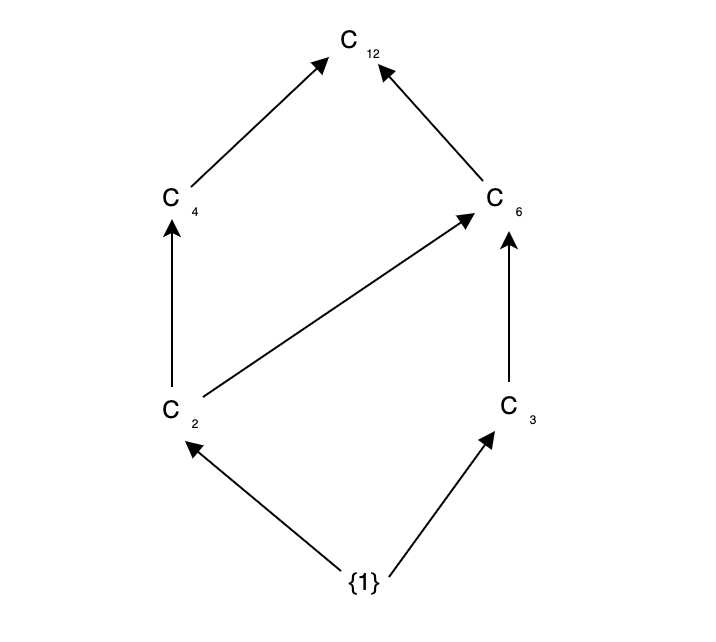
\includegraphics[width=0.85\textwidth]{./EsquemaTema3}\par\vspace{1cm}
\end{center}

\subsubsection*{Demostración}

\begin{enumerate}[label=$\circled{\arabic*}$]
\item $d \mid n, d \geq 1, <x^{\frac{n}{d}}>$ \\
Puesto que $ord( x^{\frac{n}{d}}) = \frac{n}{mcd(n, \frac{n}{d})} = \frac{n}{mcd(n,s)} = \frac{n}{s} = d$ (ya que $\frac{n}{d} = s$). \\
Entonces $|<x^{\frac{n}{d}}>| = d$. \\
Es decir, $<x^{\frac{n}{d}}> = C_{d}$.
\item $H \leqslant C_{n}, H \neq 1$ \\
$s = \min \{ r \geq 1 \mid x^{r} \in H\}$ \\
Puesto que $s \in \{r \geq 1  \mid x^{r} \in H \} \Rightarrow x^{s} \in H \Rightarrow <x^{s}> \leqslant H$ \\
Sea $x^{m} \in H$. Dividimos $m$ entre $s$,  $m = sq + t, 0 \leq t < s$: \\
$x^{m} = x^{sq} x^{t} \Rightarrow x^{t} = x^{m}(x^{sq})^{-1} \Rightarrow x^{t} \in H$ (ya que $x^{m} \in H, x^{sq} \in H$). \\
$\begin{cases}
x^{t} \in H \\
0 \leq t < s \\
s \text{ es el mínimo de } A
\end{cases}
\Rightarrow t = 0$ \\
Entonces $m = sq$ con lo que:
$$x^{m} = x^{sq} \in <x^{s}> \Rightarrow H \leqslant <x^{s}>$$
Por tanto $<x^{s}> = H$.

Puesto que $x^{n} = 1 \in H$ entonces $s \mid n$ por el mismo razonamiento anterior.
$H = <x^{s}>, s \mid n \Rightarrow n = sd \Rightarrow s = \frac{n}{d} \Rightarrow H = <x^{\frac{n}{d}}>$.
\end{enumerate}

\subsubsection*{Relación 2: Ejercicio 28}

$Sub(C_{p^{n}})$ siendo $p$ un número primo y $n \geq 1$.
$$C_{p^{n}} = < x \mid x^{p^{n}} = 1>$$
$Div(p^{n}) = \{ p^{k} \mid 0 \leq k \leq n \}$ \\
$Sub(C_{p^{n}}) = \{<x^{p^{n-k}}> = C_{p^{k}} \mid 0 \leq k \leq n>$

\subsubsection*{Relación 2: Ejercicio 27}

Describir $Sub(S_{3})$ y $Sub(D_{4})$.
$$S_{3} = \{ id, (1 \hspace{0.1cm} 2), (1\hspace{0.1cm} 3), (2 \hspace{0.1cm} 3), (1 \hspace{0.1cm} 2 \hspace{0.1cm} 3), (1 \hspace{0.1cm} 3 \hspace{0.1cm} 2) \}$$
Puesto que $|S_{3}| = 6$ entonces sus posibles subgrupos tendrán orden 1, 2, 3 ó 6.
\begin{enumerate*}
\item[Orden 1] $\{1\}$
\item[Orden 2] Como todo grupo de orden 2 es cíclico generado por un elemento de orden 2, hay tres subgrupos de orden 2: $C_{2} = <(1 \hspace{0.1cm} 2)> = \{id, (1 \hspace{0.1cm} 2)\}, \\ C'_{2} = <(1 \hspace{0.1cm} 3)> = \{id, (1 \hspace{0.1cm} 3)\}, C''_{2} = <(2 \hspace{0.1cm} 3)> = \{id, (2 \hspace{0.1cm} 3)\}$.
\item[Orden 3] Como todo grupo de orden 3 es cíclico: $C_{3} = <(1 \hspace{0.1cm} 2 \hspace{0.1cm} 3)> = \{id, (1 \hspace{0.1cm} 2 \hspace{0.1cm} 3), \\ (1 \hspace{0.1cm} 2 \hspace{0.1cm} 3)^{2} = (1 \hspace{0.1cm} 3 \hspace{0.1cm} 2)\} = <(1 \hspace{0.1cm} 3 \hspace{0.1cm} 2)> = \{id, (1 \hspace{0.1cm} 3 \hspace{0.1cm} 2), (1 \hspace{0.1cm} 3 \hspace{0.1cm} 2)^{2} = (1 \hspace{0.1cm} 2 \hspace{0.1cm} 3)\}$.
\item[Orden 6] $S_{3}$
\end{enumerate*}

$$D_{4} = <r,s \mid r^{4} = 1 = s^{2}, sr = r^{3}s> = \{1, r, r^{2}, r^{3}, s, rs, r^{2}s, r^{3}s\}$$
$|D_{4}| = 8$ y entonces buscamos subgrupos de orden 1, 2, 4 y 8.
\begin{enumerate*}
\item[Orden 1] $\{1\}$.
\item[Orden 2] Generados por elementos de orden 2 de $D_{4}$. \\
$C_{2} = <r^{2}> = \{1, r^{2} \hspace{0.5cm} C'_{2} = <s> = \{1, s\} \hspace{0.5cm} C''_{2} = <r^{2}s> = \{1, r^{2}s\}$\\
$C'''_{2} = <rs> = \{1, rs\} \hspace{0.5cm} C_{2}^{IV} = <r^{3}s> = \{1, r^{3}s\}$.
\item[Orden 4] Como los grupos de orden 4 son salvo isomorfismo $C_{4}$ o tipo Klein. Los cíclicos de orden 4 son los generados por elementos de orden 4 en $D_{4}$, que son $r$ y $r^{3}$. \\
$C_{4} = <r> = \{1, r, r^{2}, r^{3}\} = <r^{3}>$. \\
Para buscar los subgrupos en $D_{4}$ que son tipo Klein, tenemos que buscar dos elementos de orden 2 que conmutan entre sí.

$r^{2}, s$ tienen orden 2 y $sr^{i} = r^{-i}s$. \\
$K = \{1, r^{2}, s, r^{2}s\} \leqslant D_{4}$.

$r^{2}, rs$ tienen orden 2 y $r^{2}(rs) = (rs)r^{2}$. \\
$K' = \{1, r^{2}, rs, r^{3}s\} \leqslant H$.
\item[Orden 8] $D_{4}$.
\end{enumerate*}
 
% 13/04/2021

\subsubsection*{Proposición}

Sea $C_{n} = <x \mid x^{n} = 1\}$.
\begin{enumerate}[label=$\circled{\arabic*}$]
\item $<x^{m}> = <x^{mcd(m,n)}>$.
\item $<x^{m_{1}}, x^{m_{2}}, x^{m_{3}}, ..., x^{m_{k}}> = <x^{mcd(m_{1}, m_{2}, m_{3}, ..., m_{k}, n)}>$
\end{enumerate} 
 
\subsubsection*{Demostración} 

\begin{enumerate}[label=$\circled{\arabic*}$]
\item Sea $d = mcd(m, n)$, Tendremos que $n = ds$. Sabemos que $\exists !$ subgrupo cíclico de $C_{n}$ de orden $s$ que es $<x^{\frac{n}{s}}> = <x^{d}>$.
$$|<x^{m}>| = ord(x^{m}) = \frac{n}{mcd(n,m)} = \frac{n}{d} = s$$
Por tanto, $<x^{m}> = <x^{d}>$.
\item $H = <x^{m_{1}}, x^{m_{2}}, ..., x^{m_{k}}> \leqslant C_{n}$ \\
Sea $d = mcd(m_{1}, m_{2}, ..., m_{k}, n)$. \\
Puesto que $d \mid m_{i} \Rightarrow x^{mi} \in <x^{d}> \hspace{0.2cm} \forall i = 1, ..., k$ \\
Por tanto $H \leqslant <x^{d}>$. \\
Por el Teorema de Bezout, $\exists t_{1}, t_{2}, ..., t_{k}, t \in \mathbb{Z}$ tal que:
$$d = m_{1}t_{1} + m_{2}t_{2} + ... + m_{k}t_{k} + nt$$
Entonces:
$$x^{d} = x^{m_{1}t_{1}} x^{m_{2}t_{2}} ... x^{m_{k}t_{k}} \in H$$
con lo que $<x^{d}> \leqslant H$.
\end{enumerate}
 
\newpage

\section{Grupos cocientes. Teoremas de isomorfía}

\subsection{Subgrupos normales}

\subsubsection*{Definición}

Sea $G$ un grupo y $N$ un subgrupo de $G$. Diremos que $N$ es un subgrupo normal en $G$ si:
$$aN = Na \hspace{1cm} \forall a \in G$$
Es decir, las clases laterales a izquierda coinciden con las laterales a derecha.

Si $N$ es normal en $G$ lo indicaremos por $N \unlhd G$.

\subsubsection*{Ejemplos}

\begin{enumerate}[label=$\circled{\arabic*}$]
\item Si $G$ es abeliano, todo subgrupo suyo es normal.
\item Para todo $G$, $\{1\}$ y $G$ son normales.
\item Sea $G = D_{4}$ y $N = <r> = \{1, r, r^{2}, r^{3}\}$ \\
$D_{4} = <r, s \mid r^{4} = 1 = s^{2}, sr = r^{3}s >$ \\
$\sfrac{D_{4}}{N} = \{N, sN\} \hspace{2cm} \sfrac{N}{D_{4}} = \{N, Ns\}$ \\
$sN = \{s, sr, sr^{2}, sr{3}\} = \{s, r^{3}s, r^{2}s, rs\} = Ns$ \\
Por tanto $N \unlhd D_{4}$.

Sea $H = <s> = \{1, s\} \leqslant D_{4}$. No es normal en $D_{4}$:
$$rH = \{r, rs\} \neq Hr = \{r, sr\} = \{r, r^{3}s\}$$
\end{enumerate}

\subsubsection*{Teorema}

Sea $G$ un grupo y $N \leqslant G$. Son equivalentes los siguientes enunciados:
\begin{enumerate}[label=$\circled{\arabic*}$]
\item $N$ es un subgrupo normal en $G$.
\item $aNa^{-1} = N \hspace{1cm} \forall a \in G$.
\item $aNa^{-1} \leqslant N \hspace{1cm} \forall a \in H$.
\end{enumerate}
Es decir, $N$ es un subgrupo normal de $G$ si y sólo si coincide a todos sus conjugados ó, si y sólo si contiene a todos sus conjugados. \\
Para $N \leqslant G$ y $a \in G$, el subgrupo de $G$:
$$aNa^{1} = \{a x a^{-1} \mid x \in N\}$$
se llama el subgrupo conjugado de $N$ por el elemento $a$.

\subsubsection*{Demostración}

\begin{enumerate*}
\item[$\circled{1} \Rightarrow \circled{2} \Rightarrow \circled{3}$] Es fácil.
\item[$\circled{3} \Rightarrow \circled{1}$] Sea $a \in G$, tenemos que ver que
$$aN = Na$$
Lo vemos por doble inclusión.

Sea $x \in aN \Rightarrow \exists n \in N$ tal que $x = an$. \\
Entonces $xa^{-1} = ana^{-1} \in aNa^{-1} \leqslant N \Rightarrow \exists n' \in N$ tal que $x = n'a \in Na$. \\
Tenemos pues que $aN \leqslant Na$.

Sea $y \in Na \Rightarrow \exists m \in N$ tal que $y = ma$. \\
Entonces $a^{-1}y = a^{-1}ma \in a^{-1}Na \leqslant N \Rightarrow \exists m' \in N$ tal que $a^{-1}y = m' \Rightarrow y = am' \in aN$. \\
Por tanto, $Na \leqslant aN$.
\end{enumerate*}

\subsubsection*{Ejemplos}

\begin{enumerate}[label=$\circled{\arabic*}$]
\item Sea $f: G \to G'$ un homomorfismo de grupos. $Ker(f) = \{x \in G \mid f(x) = 1\}$. \\
Sea $a \in G$ y $x \in Ker(f)$:
$$f(axa^{-1}) = f(a)f(x)f(a)^{-1} ) f(a)f(a)^{-1} = 1 \Rightarrow axa^{-1} \in Ker(f)$$
Luego $aKer(f)a^{-1} \leqslant Ker(f) \hspace{0.5cm} \forall a \in G$ \\
Entonces $Ker(f) \unlhd G$.
\item Sea $G = S_{4}$ y:
$$K = \{id, (1 \hspace{0.1cm} 2)(3 \hspace{0.1cm} 4), (1 \hspace{0.1cm} 3)(2 \hspace{0.1cm} 4), (1 \hspace{0.1cm} 4)(2 \hspace{0.1cm} 3)\}$$
Sea $\alpha \in S_{4}$:
$$\alpha(1 \hspace{0.1cm} 2)(3 \hspace{0.1cm} 4) \alpha^{-1} = \alpha(1 \hspace{0.1cm} 2) \alpha^{-1} \alpha (3 \hspace{0.1cm} 4) \alpha^{-1} = (\alpha(1) \alpha(2)) (\alpha(3) \alpha(4)) \in^{\circled{*}} K$$
$\circled{*} \Rightarrow \alpha$ es biyectiva.

Análogamente, por el mismo argumento:
$$\alpha)1 \hspace{0.1cm} 3)(2 \hspace{0.1cm} 4) \alpha^{-1} \in K, \alpha(1 \hspace{0.1cm} 4)(2 \hspace{0.1cm} 3) \in K$$
$$\alpha id \alpha^{-1} = id \in K$$
Por tanto, $\alpha K \alpha^{-1} \leqslant K \hspace{0.5cm} \forall \alpha \in S_{4} \Rightarrow K \unlhd S_{4}$.
\end{enumerate}

\subsubsection*{Proposición}

Sea $G$ un grupo y $X \subset G$ un subconjunto de $G$ no vacío. Sea $N = <X>$.
$$N \unlhd G \iff axa^{-1} \in N \hspace{0.5cm} \forall a \in G \hspace{0.2cm} \forall x \in X$$

\subsubsection*{Demostración}

\begin{enumerate*}
\item[$\Leftarrow$] Obvio.
\item[$\Rightarrow$] Sea $a \in G$ y sea:
$$\varphi_{a}: G \to G \hspace{1cm} \varphi_{a}(y) := aya^{-1}$$
Es fácil ver (ejercicio) que $\varphi_{a}$ es un homomorfismo de grupos.
$$aNa^{-1} = (\varphi_{a})_{*}(N) = (\varphi_{a})_{*}(<X>) =$$ $$= <(\varphi_{a})_{*}(X)> = <aXa^{-1}> \leqslant N$$
Por tanto $N \unlhd G$.
\end{enumerate*}

\subsubsection*{Proposición}

$\forall n \geq 2 \hspace{1cm} A_{n} \unlhd S_{n}$

\subsubsection*{Demostración}

Utilizaremos que $A_{n}$ está generado por:
$$X = \{(x_{1}, x_{2}, x_{3}) \mid x_{1}, x_{2}, x_{3} \in \{1, 2, ..., n\}\}$$
Sea $\alpha \in S_{n}$ y $(x_{1} \hspace{0.1cm} x_{2} \hspace{0.1cm} x_{3}) \in X$, entonces:
$$\alpha(x_{1} \hspace{0.1cm} x_{2} \hspace{0.1cm} x_{3}) \alpha^{-1} = (\alpha(x_{1}) \alpha(x_{2}) \alpha(x_{3})) \in X \subset A_{n}$$
Por tanto, $A_{n} \unlhd S_{n}$:
$$(x \hspace{0.1cm} y)(z \hspace{0.1cm} t) = (x \hspace{0.1cm} y \hspace{0.1cm} z)(y \hspace{0.1cm} < \hspace{0.1cm} t)$$
$$(x \hspace{0.1cm} y)(y \hspace{0.1cm} z) = (x \hspace{0.1cm} y \hspace{0.1cm} z)$$

% 14/04/2021

\subsubsection*{Relación 3: Ejercicio 3}

Sea $G$ finito y $H \leqslant G$ tal que $[G:H] = 2 \Rightarrow H \unlhd G$.

$[G:H] = 2 \Rightarrow
\begin{cases}
\sfrac{G}{H} = \{H, aH\} \hspace{0.5cm} a \notin H \\
\sfrac{H}{G} = \{H, Ha\}
\end{cases}$ \\
Como 
$\begin{cases}
G = H \cup aH \\
G = H \cup Ha
\end{cases}$ 
y ambas uniones son disjuntas $\Rightarrow H = H$ y $ aH = Ha$. \\
Entonces $H \unlhd G$.

Por tanto $A_{n} \unlhd S_{n} \hspace{0.2cm} \forall n \geq 2$ pues $[S_{n}:A_{n}] = 2$. También obtenemos que en:
$$D_{n} = <r,s \mid r^{n} = 1 = s^{2}, sr=r^{n-1}s>$$
el grupo $N = <r> \unlhd D_{n}$ pues $[D_{n}:N] = \frac{|D_{n}|}{|N|} = \frac{2n}{n} = 2$.

\subsubsection*{Relación 3: Ejercicio 4}

Describid el retículo de subgrupos de $A_{4}$.

$A_{4} = \{id, (1 \hspace{0.1cm} 2)(3 \hspace{0.1cm} 4), (1 \hspace{0.1cm} 3)(2 \hspace{0.1cm} 4), (1 \hspace{0.1cm} 2 \hspace{0.1cm} 3), (1 \hspace{0.1cm} 3 \hspace{0.1cm} 2), (1 \hspace{0.1cm} 2 \hspace{0.1cm} 4), (1 \hspace{0.1cm} 4 \hspace{0.1cm} 2), (1 \hspace{0.1cm} 3 \hspace{0.1cm} 4), (1 \hspace{0.1cm} 4 \hspace{0.1cm} 3), \\ (2 \hspace{0.1cm} 3 \hspace{0.1cm} 4), (2 \hspace{0.1cm} 4 \hspace{0.1cm} 3)\}$

$|A_{4}| = 2 \Rightarrow$ Tendrá posiblemente subgrupos en orden 1, 2, 3, 4, 6 ó 12.

$K = \{id, (1 \hspace{0.1cm} 2)(3 \hspace{0.1cm} 4), (1 \hspace{0.1cm} 3)(2 \hspace{0.1cm} 4), (1 \hspace{0.1cm} 4)(2 \hspace{0.1cm} 3)\} \unlhd A_{4}$.

$A_{4}$ no tiene subgrupos de orden 6.

Supongamos que $\exists N \leqslant A_{4}$ tal que $|N| = 6$. Entonces $[A_{4}:N] = \frac{|A_{4}|}{|N|} = \frac{12}{6} = 2 \Rightarrow N \unlhd A_{4}$. \\
Como $|N| = 6, N$ ha de contener un ciclo de longitud 3. Supongamos:
$$(1 \hspace{0.1cm} 2 \hspace{0.1cm} 3) \in N \Rightarrow (1 \hspace{0.1cm} 2 \hspace{0.1cm} 3) = (1 \hspace{0.1cm} 3 \hspace{0.1cm} 2) \in N$$

Sea $\alpha = (1 \hspace{0.1cm} 2)(3 \hspace{0.1cm} 4) \in A_{4}$, como $N \unlhd A_{4}$, entonces:
$$\alpha (1 \hspace{0.1cm} 2 \hspace{0.1cm} 3) \alpha^{-1} = (2 \hspace{0.1cm} 1 \hspace{0.1cm} 4) = (1 \hspace{0.1cm} 4 \hspace{0.1cm} 2) \in N \Rightarrow (1 \hspace{0.1cm} 4 \hspace{0.1cm} 2)^{-1} = (1 \hspace{0.1cm} 2 \hspace{0.1cm} 4) \in N$$

Sea $\beta = (1 \hspace{0.1cm} 3)(2 \hspace{0.1cm} 4) \in A_{4}$, como $N \unlhd A_{4}$, entonces:
$$\beta(1 \hspace{0.1cm} 2 \hspace{0.1cm} 3) \beta^{-1} = (3 \hspace{0.1cm} 4 \hspace{0.1cm} 1) = (1 \hspace{0.1cm} 3 \hspace{0.1cm} 4) \in N \Rightarrow (1 \hspace{0.1cm} 3 \hspace{0.1cm} 4)^{-1} = (1 \hspace{0.1cm} 4 \hspace{0.1cm} 3) \in N$$

Como $id \in N$, pues $N$ es un subgrupo, resulta $|N| \geq 7$ (Contradicción).

Los subgrupos normales de $A_{4}$ son $\{1\}, A_{4}, y K$. \\
Los de orden 2 y los de orden 3 no son normales en $A_{4}$.
$$C_{2} = \{id, (1 \hspace{0.1cm} 2)(3 \hspace{0.1cm} 4)\} \leqslant A_{4}$$
Sea $\alpha = (1 \hspace{0.1cm} 2 \hspace{0.1cm} 3)$, entonces:
$$\alpha (1 \hspace{0.1cm} 2)(3 \hspace{0.1cm} 4) \alpha^{-1} = \alpha(1 \hspace{0.1cm} 2) \alpha^{-1} \alpha (3 \hspace{0.1cm} 4) \alpha^{-1} = (2 \hspace{0.1cm} 3)(1 \hspace{0.1cm} 4) = (1 \hspace{0.1cm} 4)(2 \hspace{0.1cm} 3) \notin C_{2}$$
$\alpha C_{2} \alpha^{-1} \nleqslant C_{2} \Rightarrow C_{2} \ntrianglelefteq A_{4}$ \\
$\begin{cases}
C_{2} \leqslant K \\
K \text{ es abeliano}
\end{cases}$
entonces $C_{2} \unlhd K$.

\subsection{Grupo Cociente}

\subsubsection*{Definición}

Sea $G$ un grupo y $N \unlhd G$. Consideramos:
$$\sfrac{G}{N} = \{aN \mid a \in G\}$$
Definimos en $\sfrac{G}{N}$ la siguiente operación binaria:
$$\sfrac{G}{N} \times \sfrac{G}{N} \to \sfrac{G}{N}$$
$$(aN, bN) \mapsto (aN)(bN) := abN$$

Por ser $N$ un subgrupo normal de $G$, esta operación está bien definida. En efecto:
\begin{equation*}
\begin{cases}
aN = a_{1}N \\
bN = b_{1}N
\end{cases}
\Rightarrow abN = a_{1}b_{1}N
\end{equation*}
$aN = a_{1}N \iff a_{1}^{-1}a \in N \iff \exists n \in \mathbb{N}$ tal que $a_{1}^{-1}a = n \iff a = a_{1}n$ \\
$bN = b_{1}N \iff \exists m \in N$ tal que $b = b_{1} m$. \\
Entonces $ab = a_{1}nb_{1}m$. \\
Como $nb_{1} \in Nb_{1} = b_{1}N \Rightarrow \exists n' \in N$ tal que $nb_{1} = b_{1}n'$. \\
Entonces $ab = a_{1}nb_{1}m = a_{1}b_{1}n'm \Rightarrow (a_{1}b_{1})^{-1}(ab) \in N \Rightarrow abN = a_{1}b_{1}N$.

Resulta que $\sfrac{G}{N}$ con este producto tiene estructura de grupo, con uno dado por $1N = N$ y donde para cada $aN \in \sfrac{G}{N}, (aN)^{-1} = a^{-1}N$. \\
Este grupo lo llamaremos el grupo cociente de $G$ por $N$.

Se tiene un epimorfismo de grupos:
$$p: G \to \sfrac{G}{N} \hspace{1cm} p(a) := aN$$
que llamaremos la proyección canónica.

\subsubsection*{Teorema}

Sea $f: G \to G'$ un homomorfismo de grupos. Sea $N \unlhd G$ tal que $N \leqslant Ker(f)$, entonces:
\begin{enumerate}[label=$\circled{\arabic*}$]
\item Existe un único homomorfismo:
$$\bar{f}: \sfrac{G}{N} \to G'$$
tal que $\bar{f}_{o}p = f$.
\begin{center}
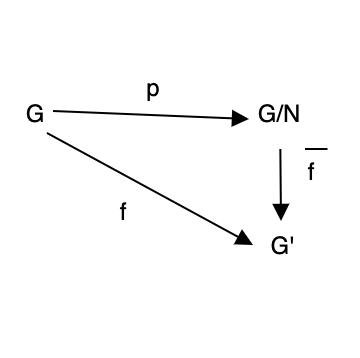
\includegraphics[width=0.25\textwidth]{./Tema4_1}\par\vspace{1cm}
\end{center}
\item $\bar{f}$ es epimorfismo $\iff f$ es epimorfismo.
\item $\bar{f}$ es monomorfismo $\iff N = Ker(f)$.
\end{enumerate}

$\bar{f}$ se llama el homomorfismo inducido por $f$ en el grupo cociente $\sfrac{G}{N}$.

\subsubsection*{Demostración}

$$f: G \to G'$$
$$N \unlhd G \text{ tal que } N \leqslant Ker(f)$$
\begin{enumerate}[label=$\circled{\arabic*}$]
\item Definimos:
$$\bar{f}: \sfrac{G}{N} \to G' \text{ por } \bar{f}(aN) := f(a)$$
Veamos $\bar{f}$ está bien definido: \\
Si $aN = bN \iff b^{-1}a \in N \Rightarrow b^{-1}a \in Ker(f) \Rightarrow f(b^{-1}a) = f(b^{-1})f(a) = 1 \Rightarrow f(a) = f(b)$. \\
Es fácil ver que $\bar{f}$ es un homomorfismo así como que $\bar{f}_{o}p = f$.

Supongamos que $g: \sfrac{G}{N} \to G'$ homomorfismo tal que $g_{o}p = f$.
$$\bar{f}: \sfrac{G}{N} \to G'$$
Sea $aN \in \sfrac{G}{N}$, entonces:
$$g(aN) = g(p(a)) = (g_{o}p)(a) = f(a) = \bar{f}(aN)$$
Por tanto, $\bar{f} = g$.

\item Puesto que $Img(\bar{f}) = Img(f)$.
$\begin{cases}
\bar{f}: \sfrac{G}{N} \to G' \\
\bar{f}(aN) = f(a)
\end{cases}$
entonces $\bar{f}$ es epimorfismo $\iff Img(\bar{f}) = G' \iff Img(f) = G' \iff f$ es epimorfismo.

\item $\bar{f}$ es monomorfimos $\iff N = Ker(f)$.
\begin{enumerate*}
\item[$\Rightarrow$] Tenemos que ver que $Ker(f)  \leqslant N$. Sea $a \in Ker(f) \Rightarrow f(a) = 1$ \\
Como $\bar{f}(aN) = f(a) = 1 \Rightarrow aN \in Ker(\bar{f}) =^{\circled{*}} \{N\} \Rightarrow \\ \Rightarrow aN = N \Rightarrow a \in N$ \\
$\circled{*} \Rightarrow \bar{f}$ es monomorfismo.
\item[$\Leftarrow$] Si $N = Ker(f), \bar{f}: \sfrac{G}{N} \to G'$. \\
Sea $aN \in \sfrac{G}{N}$ tal que $\bar{f}(aN) = f(a) = 1$. Entonces:
$$a = Ker(f) = N \Rightarrow aN = N$$
Así pues $Ker(\bar{f}) = \{N\}$ y $\bar{f}$ es monomorfismo.
\end{enumerate*}
\end{enumerate}

\subsubsection*{Corolario: Primer Teorema de Isomorfia}

Sea $f: G \to G'$ un homomorfismo de grupos. \\
Entonces $f$ induce un isomorfismo:
$$\sfrac{G}{Ker(f)} \equiv Img(f) \hspace{1cm} aKer(f) \mapsto f(a)$$

\subsubsection*{Demostración}

Consideramos $f: G \to Img(f)$ y aplicamos el teorema anterior a este homomorfismo tomando $N = Ker(f)$. \\
$f$ induce un homomorfismo:
$$\bar{f}: \sfrac{G}{Ker(f)} \to Img(f) \hspace{1cm} \bar{f}(aKer(f)) = f(a)$$
$\bar{f}$ es epimorfismo por $\circled{2}$. \\
Como $N = Ker(f), \bar{f}$ es monomorfismo por $\circled{3}$.

\subsubsection*{Relación 3: Ejercicio 12}

$G$ y $H$ finitos y $mcd(|G|, |H|) = 1$. \\
Probar que si $f: G \to H$ es un homomorfismo entonces $f(a) = 1 \hspace{0.2cm} \forall a \in G$.

$\sfrac{G}{Ker(f)} \equiv Img(f) \Rightarrow \frac{|G|}{|Ker(f)|} = |\sfrac{G}{Ker(f)} = |Img(f)| \Rightarrow \\ \Rightarrow |G| = |Ker(f)||Img(f)|$ \\
$\begin{cases}
\text{En particular, } |Img(f)| \text{ es divisor de } |G| \\
Img(f) \leqslant H \Rightarrow |Img(f)| \text{ es divisor de } |H|
\end{cases}
\Rightarrow |Img(f)| = 1 \Rightarrow \\ \Rightarrow Img(f) = \{1\}$ \\
Por tanto $f(a) = 1 \hspace{0.2cm} \forall a \in G$

\subsubsection*{Corolario}

Si $f: G \to G'$ es un homomorfismo y $G$ y $G'$ son finitos, entonces:
$$|G| = |Img(f)||Ker(f)|$$

Vamos a estudiar quien es $Sub(\sfrac{G}{N})$ en relación con $Sub(G)$.

\subsubsection*{Proposición}

Sea $G$ un grupo y $N \unlhd G$. Entonces:
\begin{enumerate}[label = $\circled{\arabic*}$]
\item Si $H \in Sub(G)$ tal que $N \leqslant H$ entones $N \unlhd H$ y $\sfrac{H}{N} \in Sub(\sfrac{G}{N})$.
\item Si $H_{1}, H_{2} \in Sub(G)$ tal que $N \unlhd H_{i} \hspace{0.2cm} i = 1, 2$, entonces:
$$\sfrac{H_{i}}{N} = \sfrac{H_{2}}{N} \iff H_{1} = H_{2}$$
\item Sea $L \in Sub(\sfrac{G}{N})$ entonces existe un único $H \in Sub(G)$ tal que $N \unlhd H$ y $L = \sfrac{H}{N}$.
\end{enumerate}

$Sub(\sfrac{G}{N}) = \{\sfrac{H}{N} \mid N \unlhd H \leqslant G\}$

\subsubsection*{Demostración}

\begin{enumerate}[label = $\circled{\arabic*}$]
\item Si $aNa^{-1} \leqslant N \hspace{0.2cm} \forall a \in G$ entonces $aNa^{-1} \leqslant N \hspace{0.2cm} \forall a \in H$ pues $H \leqslant G$, con lo que $N \unlhd H$. \\
Podemos pues considerar $\sfrac{H}{N} \leqslant \sfrac{G}{N}$ claramente. \\
Así $\sfrac{H}{N} \in Sub(\sfrac{G}{N})$.
\item
\begin{enumerate*}
\item[$\Leftarrow$] Es obvio.
\item[$\Rightarrow$] $H_{1}, H_{2} \leqslant G$ tal que $N \unlhd H_{1} \hspace{0.2cm} \forall i = 1,2$ \\
$\sfrac{H_{1}}{N} = \sfrac{H_{2}}{N} $ \\
Sea $a \in H_{1} \Rightarrow aN \in \sfrac{H_{1}}{N} = \sfrac{H_{2}}{N} \Rightarrow \exists b \in H_{2}$ tal que $aN = bN \iff b^{-1}a \in N \leqslant H_{2}$.
\begin{equation*}
\begin{cases}
b^{-1}a \in H_{2} \\
b \in H_{2}
\end{cases}
\Rightarrow a = b(b^{-1}a) \in H_{2}
\end{equation*}
Tenemos que $H_{1} \leqslant H_{2}$. De la misma forma se demuestra que $H_{2} \leqslant H_{1}$ y entonces $H_{1} = H_{2}$.
\end{enumerate*}
\item $L \leqslant \sfrac{G}{N}$ \\
Consideramos la proyección canónica:
$$p: G \to \sfrac{G}{N} \hspace{1cm} p(a) = aN$$
$L \leqslant \sfrac{G}{N}$ entonces $p^{*}(L) \leqslant G$. \\
Sea $H = p^{*}(L) = \{a \in G \mid p(a) \in L\} = \{a \in G \mid aN \in L\} \leqslant G$.
Sea $a \in N \Rightarrow p(a) = aN = N \in L \Rightarrow a \in H$ \\
por tanto $N \leqslant H$.

Veamos que $L = \sfrac{H}{N}$. \\
Es claro que $\sfrac{H}{N} \leqslant L$. \\
Recíprocamente, si $aN \in L \Rightarrow a \in H \Rightarrow aN \in \sfrac{H}{N}$, es decir, $L \leqslant \sfrac{H}{N}$. \\
La unicidad es consecuencia de $\circled{2}$.
\end{enumerate}

\subsubsection*{Segundo Teorema de Isomorfia}

Sea $G$ un grupo y $N \unlhd G$. \\
Sea $H \in Sub(G)$ tal que $N \leqslant H$. \\
Entonces:
$$\sfrac{H}{N} \unlhd \sfrac{G}{N} \iff H \unlhd G$$
Además en tal caso:
$$\sfrac{G}{H} \equiv \sfrac{(\sfrac{G}{N})}{(\sfrac{H}{N})}$$

% 19/04/2021

\subsubsection*{Demostración}

$N \unlhd G$ y $H \leqslant G$ con $N \unlhd H$.
\begin{enumerate*}
\item[$\Leftarrow)$] $H \unlhd G$ y tenemos que ver que $\sfrac{H}{N} \unlhd \sfrac{G}{N}$. \\
Sean $aN \in \sfrac{H}{N}, xN \in \sfrac{G}{N}$, es decir, $a \in H$. \\
$(xN)(aN)(xN)^{-1} = (xax^{-1})N \in \sfrac{H}{N} \\
\begin{cases}
a \in H \\
x \in G \\
H \unlhd G
\end{cases}
\Rightarrow xHx^{-1} \leqslant H$ y por tanto $xax^{-1} \in H$. \\
Es decir, $(xN) \sfrac{H}{N} (xN)^{-1} \leqslant \sfrac{H}{N} \forall xN \in \sfrac{G}{N} \Rightarrow \sfrac{H}{N} \unlhd \sfrac{G}{N}$.
\item[$\Rightarrow)$] Suponemos que $\sfrac{H}{N} \unlhd \sfrac{G}{N}$. Consideramos las proyecciones canónicas: 
$$G \overset{p}{\to} \sfrac{G}{N} \overset{q}{\to} \sfrac{(\sfrac{G}{N})}{(\sfrac{H}{N})}$$
Sea $f = q_{o}p: G \to \sfrac{(\sfrac{G}{N})}{(\sfrac{H}{N})}$.
$$f(a) = (aN)\sfrac{H}{N}$$
$f$ es un epimorfismo por ser composición de epimorfismos.
$$Ker(f) = \{a \in G \mid f(a) = \sfrac{H}{N}\} = \{a \in G \mid (aN)\sfrac{H}{N} = \sfrac{H}{N}\} =$$ $$= \{a \in G \mid aN \in \sfrac{H}{N}\}$$
Veamos que $H = Ker(f)$ por doble inclusión. Es claro que $H \leqslant Ker(f)$. Sea $a \in Ker(f)$ entonces $aN \in \sfrac{H}{N} \Rightarrow \exists b \in H$ tal que $aN = bN \iff 
\begin{cases}
b^{-1}a \in N \leqslant H \\
b \in H
\end{cases}
\Rightarrow a = b(b^{-1}a) \in H$. \\
Por tanto $Ker(f) \leqslant H$.

Consecuentemente, $H = Ker(f) \Rightarrow H \unlhd G$. \\
Además, aplicando el 1º Teorema de Isomorfia a $f$:
$$\sfrac{G}{Ker(f)} \equiv Img(f)$$
es decir,
$$\sfrac{G}{H} \equiv \sfrac{(\sfrac{G}{N})}{(\sfrac{H}{N})}$$
pues $f$ es epimorfimo.
\end{enumerate*}

\subsubsection*{Tercer Teorema de Isomorfia}

Sea $G$ un grupo y $N, K \in Sub(G)$ con $N \unlhd G$. Entonces:
\begin{enumerate}[label=$(\arabic*)$]
\item $KN$ es un subgrupo de $G$ y $N \unlhd KN$.
\item $K \cap N \unlhd K$.
\item Existe un isomorfismo:
$$\sfrac{K}{K \cap N} \equiv \sfrac{KN}{N}$$
\end{enumerate}

\subsubsection*{Demostración}

\begin{enumerate*}
\item[(1)] Para demostrar que $KN \leqslant G$, basta con ver que $KN = NK$ y esta igualdad es inmediata puesto que $N \unlhd G$. \\
Por tanto $KN \in Sub(G)$. \\
Es claro que $N \leqslant KN (x \in N, x = 1 \cdot x \in KN)$ y $N \unlhd G$, entonces $N \unlhd KN$.
\item[(2) y (3)] Consideramos los homomorfismos:
$$K \overset{i}{\hookrightarrow} G \overset{p}{\to} \sfrac{G}{N}$$
y sea $g = p_{o}i: K \to \sfrac{G}{N}$.
$$g(a) = aN \hspace{0.2cm} \forall a \in K$$
$Ker(g) = \{a \in K \mid g(a) = N \} = \{a \in K \mid aN = N\} = \{a \in K \mid a \in N\} = K \cap N$ \\
y entonces $K \cap N \unlhd K$ y tenemos $(2)$. \\
Además, por el 1º Teorema de Isomorfia aplicada a $g$:
$$\sfrac{K}{K \cap N} \equiv Img(g)$$
$Img(g) = \{g(a) \mid a \in K\} = \{aN \mid a \in K\} \overset{?}{=} \sfrac{KN}{N}$ \\
Puesto que $K \leqslant KN$, es claro que $Img(g) \leqslant \sfrac{KN}{N}$. \\
Recíprocamente, sea $xN \in \sfrac{KN}{N}$ es decir $x \in KN$. \\
Si $x \in KN \Rightarrow \exists a \in K$ y $\exists b \in N$ tal que $x = ab$. \\
Entonces:
$$xN = (ab)N = (aN)(bN) \overset{b \in N}{=} (aN)N = aN \overset{a \in K}{\in} Img(g)$$
$\sfrac{KN}{N} \leqslant Img(g)$
$$\sfrac{K}{K \cap N} \equiv \sfrac{KN}{N}$$ 
\end{enumerate*}

\subsubsection*{Relación 3: Ejercicio 14}

$G$ un grupo, $N \unlhd G$ tal que $N$ y $\sfrac{G}{N}$ son abelianos. $H \leqslant G$. \\
Demostrad que $\exists K \unlhd H$ tal que $K$ y $\sfrac{H}{K}$ son abelianos.

$G, N, H \in Sub(G), N \unlhd G$. \\
$N \cap H \unlhd H$ y $\sfrac{NH}{N} \equiv \sfrac{H}{N \cap H}$ (3º Teorema de Isomorfia). \\
Tomamos $K = N \cap H \leqslant H$. \\
Como $K \leqslant N$ y $N$ abeliano $\Rightarrow K$ es abeliano. \\
Por otro lado $\sfrac{H}{K} = \sfrac{H}{N \cap K} \equiv \sfrac{HN}{N} \leqslant \sfrac{G}{N}$ \\
Como $\sfrac{G}{N}$ es abeliano, entonces $\sfrac{HN}{N}$ es abeliano $\Rightarrow \sfrac{H}{K}$ es abeliano.

\subsubsection*{Relación 3: Ejercicio 15}

$G$ grupo finito, $K, N \in Sub(G)$ con $N \unlhd G$. Suponemos que $|K|$ y $[G:N]$ son primos relativos. \\
Demostrad que $K \leqslant N$.

Sabemos que
$$\sfrac{K}{K \cap N} \equiv \sfrac{KN}{N} (\text{3º Teorema de Isomorfia)}$$
entonces
$$[K : K \cap N] = [KN : N] = r$$
Como
$$\sfrac{KN}{N} \leqslant \sfrac{G}{N} \Rightarrow r = |\sfrac{KN}{N}| \mid |\sfrac{G}{N}| = [G:N]$$
Por otro lado
$$r = [K:K \cap N] = \frac{|K|}{|K \cap N|} \Rightarrow |K| = r \cdot |K \cap N| \Rightarrow r \mid |K|$$
Como $mcd(|K|, [G:N]) = 1$, entonces $r = 1$. \\
Tenemos entonces $|\sfrac{K}{K \cap N}| = 1 \Rightarrow K = K \cap N$.

% 20/04/2021

\subsubsection*{Definición}

Sea $G$ un grupo. Se define su centro como:
$$Z(G) = \{a \in G \mid ax = xa \hspace{0.2cm} \forall x \in G\}$$

\subsubsection*{Propiedades}

\begin{itemize}
\item $Z(G) \unlhd G$ (Relación 3: Ejercicio 6)
\item G es abeliano $\iff Z(G) = G$.
\end{itemize}

\subsubsection*{Relación 3: Ejercicio 8}

Demostrar que $Z(A_{3}) = A_{3}$ y $Z(A_{n}) = \{id\} \hspace{0.2cm} \forall n \geq 4$.

$A_{3} = \{id, (1 \hspace{0.1cm} 2 \hspace{0.1cm} 3), (1 \hspace{0.1cm} 3 \hspace{0.1cm} 2)\} = <(1 \hspace{0.1cm} 2 \hspace{0.1cm} 3)>$ es abeliano y entonces $Z(A_{3}) = A_{3}$.

Sea $n \geq 4$ y  sea $\sigma \in A_{n}, \sigma \neq id$ entonces $\exists \alpha \in A_{n}$ tal que $\sigma\alpha \neq \alpha\sigma$. \\
Si $\sigma \neq id$ entonces $\exists i, j \in \{1, 2, ..., n\}$ tal que $\sigma(i) = j$ siendo $j \neq i$. \\
Elegimos $k, l \in \{1, 2, ..., n\}$ tal que $k \neq l$ y $\{k, e\} \cap \{i, j\} \neq \emptyset$ (odemos elegirlos porque $n \geq 4$). \\
Sea $\alpha = (k \hspace{0.1cm} k \hspace{0.1cm} l) \in A_{n}$ \\
$\begin{cases}
\sigma \alpha (i) = \sigma(i) = j \\
\alpha \sigma (i) = \alpha(j) = k
\end{cases}
\Rightarrow \sigma \alpha (i) \neq \alpha \sigma (i) \Rightarrow \sigma \alpha \neq \alpha \sigma \Rightarrow \sigma \notin Z(A_{n})$

Consecuentemente $Z(A_{n}) = \{id\} \hspace{0.2cm} \forall n \geq 4$

\subsubsection*{Relación 3: Ejercicio 9}

Demostrar que:
\begin{enumerate}[label=$\alph*)$]
\item $Z(D_{n}) = \{1, r^{m}\}$ si $n = 2m$
\item $Z(D_{n}) = \{1\}$ si $n = 2m + 1$
\end{enumerate}

\begin{enumerate}[label=$\alph*)$]
\item $n = 2m$ \\
$D_{n} = <r,s \mid r^{n} = 1 = s^{2}, sr = r^{-1}s> = \{1, r, ..., r^{n-1}, s, rs, ..., r^{n-1}s\}$ \\
Observamos primero que $r^{k}s \notin Z(D_{n}) \forall k = 0, ..., n-1$
$$r(r^{k}s) = r^{k+1}s \hspace{1cm} (r^{k}s)r = r^{k}r^{-1}s = r^{k-1}s$$
$r^{k+1}s = r^{k-1}s \iff r^{k+1} = r^{k-1} \iff r = r^{-1} \iff r^{2} = 1 \iff ord(r) = 2 \neq n$ (Contradicción)
$$r(r^{k}s) \neq (r^{k}s)r \Rightarrow r^{k}s \notin Z(D_{n}) \forall k = 0, ..., n-1$$

Obviamente $r^{k}r^{j} = r^{j}r^{k} \hspace{0.2cm} \forall j = 0, ..., n-1$. \\
Por tanto decir que $r^{k} \in Z(D_{n})$ es decir
$$r^{k}(r^{j}s) = (r^{j}s)r^{k} \iff r^{k+j}s = r^{j}r^{-k}s = r^{j-k}s \iff$$ $$\iff r^{k+j} = r^{j-k} \hspace{0.2cm} \forall j \iff r^{k} = r^{-k} \iff (r^{k})^{2} = 1 \iff$$ $$\iff ord(r^{k}) = 2$$
Sabemos que $ord(r^{k}) = \frac{n}{mcd(n,k)}$
$$r^{k} \in Z(D_{n}) \iff \frac{n}{mcd(n,k)} = 2 \iff n = 2 mcd(n,k)$$
Como $n = 2m$
$$2m = 2 mcd(2m,k) \iff m = mcd(2m, k) \iff k = m$$
$$Z(D_{2m}) = \{1, r^{m}\}$$
\end{enumerate}

\subsubsection*{Definición}

Sea $G$ un grupo. Un automorfismo de $G$ es un isomorfismo $f: G \to G$
$$Aut(G) = \{f: G \to G \mid f \text{ es automorfismo}\}$$
$Aut(G)$ con la composición es un grupo.

\subsubsection*{Relación 3: Ejercicio 18}

Sea $n \geq 2$ y $C_{n} = <x \mid x^{n} = 1> = \{1, x, ..., x^{n-1}\}$. \\
Sea $G$ un grupo arbitrario. Demostrar que:
\begin{enumerate}[label = $(\arabic*)$]
\item Si $\theta: C_{n} \to G$ es un homomorfismo de grupo con $\theta(x) = g (g \in G)$ entonces
$$ord(g) \mid n \text{ y } \theta(x^{k}) = g^{k} \hspace{0.2cm} \forall k = 0, ..., n-1$$
Puesto que $\theta$ es un homomorfismo
$$1 = \theta(1) = \theta(x^{n}) = \theta(x)^{n} = g^{n}$$
Por tanto $g$ es un elemento de $G$ de orden finito y además, $ord(g) \mid n$.
\item Demostrar que para cada $g \in G$ tal que $ord(g) \mid n$ existe un único homomorfismo de grupos.
$$\theta_{g}: C_{n} \to G \text{ tal que } \theta_{g}(x) = g$$
Definimos $\theta_{g}: C_{n} \to G$ por $\theta_{g}(x^{k}) := g^{k} \hspace{0.2cm} k = 0, ..., n-1$. \\
Veamos que $\theta_{g}$ es un homomorfismo.

$x^{k}, x^{r} \in C_{n}$ hemos de ver que $\theta_{g}(x^{k} \cdot x^{r}) = \theta_{g}(x^{k}) \theta_{g}(x^{r})$
$$\theta_{g}(x^{k} \cdot x^{r}) = \theta_{g}(x^{\text{res}(k+r;n)}) = g^{\text{res}(k+r;n)} = g^{s}$$
donde $s = \text{res}(k+r;n)$. \\
Sea $ord(g) = t$
$$\theta_{g}(x^{k}) \cdot \theta_{g}(x^{r}) = g^{k} \cdot g^{r} = g^{\text{res}(x+r;t)}$$
$s = tq + h \hspace{0.5cm} h = \text{res}(s;t) \hspace{0.5cm} 0 \leq h \leq t - 1$ \\
$s = \text{res}(k+r;n)$ entonces $k+r=nq'+s \hspace{0.5cm} 0 \leq s \leq n-1$ \\
Como $ord(g) = t \mid n \Rightarrow n = tq''$. \\
$k+r = nq' + s = tq''q' + s = tq''q' + tq + h = t(q''q' +q)+h$ con $0 \leq h \leq t-1 \Rightarrow$ res$(k+r;t) = h = $ res$(s;t)$

Entonces $\theta_{g}(x^{k}x^{r}) = \theta_{g}(x^{k}) \theta_{g}(x^{r})$.

La unidad es consecuencia de $(1)$.

\item Sea $g \in G$ tal que $ord(g) \mid n$. Demostrar que $\theta_{g}: C_{n} \to G$ es monomorfismo $\iff ord(g) = n$.
$$\theta_{g}: C_{n} \to G \hspace{0.2cm} \theta_{g}(x^{k}) = g^{k} \hspace{0.2cm} \forall k$$
\begin{enumerate*}
\item[$\Rightarrow)$] Suponemos que $\theta_{g}$ es monomorfismo $\Rightarrow Ker(\theta_{g}) = \{1\}$.

Sea $t = ord(g)$, entonces $g^{t} = 1$. \\
Entonces:
$$1 = g^{t} = \theta(x^{t}) \Rightarrow x^{t} \in Ker(\theta_{g}) = \{1\} \Rightarrow x^{t} = 1 \overset{ord(x) = n}{\Rightarrow} n \mid t$$
Como $t \mid n \Rightarrow n = t$.

% 21/04/2021

\item[$\Leftarrow)$] $ord(g) = n \hspace{0.5cm} \theta_{g}: C_{n} \to G, \theta_{g}(x^{k}) = g^{k}$ \\
Sea $x^{k} \in Ker(\theta_{g}) \Rightarrow \theta_{g}(x^{k}) = g^{k} = 1 \Rightarrow 
\begin{cases}
n \mid k \\
0 \leq k \leq n-1
\end{cases}
\Rightarrow \\ \Rightarrow k = 0$, es decir, $x^{k} = 1$. \\
Por tanto $Ker(\theta_{g}) = \{1\} \Rightarrow \theta_{g}$  es monomorfismo.
\end{enumerate*}
\item Demostrar que existe un isomorfismo
$$U(\mathbb{Z}_{n}) \equiv Aut(C_{n})$$
dado por $r \mapsto f_{\sigma}: C_{n} \to C_{n}, f_{r}(x) = x^{r}$. \\
En particular $Aut(C_{n})$ es abeliano y tiene $\varphi(n)$ elementos ($\varphi$ función de Euler).
$$U(\mathbb{Z}_{n}) = \{r \mid 1 \leq r \leq n-1 \text{ y } mcd(n,r) = 1\}$$
Entonces para $r \in U(\mathbb{Z}_{n}), x^{r}$ es un generador de $C_{n}$ pues $ord(x^{r}) = \frac{n}{mcd(n,r)} = \frac{n}{1} = n$. \\
Por $(2)$ $f_{r}: C_{n} \to C_{n}, f_{r}(x) = x^{r} (f_{r}(x^{k} = x^{kr})$ y $(3)$, es un monomofrismo. \\
Como $Img(f_{r}) = <f_{r}(x)> = <x^{r}> = C_{n}$, entonces $f_{r}$ también es epimorfismo.

Tenemos pues una aplicación
$$f: U(\mathbb{Z_{n}} \to Aut(C_{n}), r \mapsto f_{r}$$
$f$ es un homomorfismo de grupos.
$$f(rs) = f_{rs}: C_{n} \to C_{n}$$
$$f(r)_{o}f(s) = f_{r} o f_{s}: C_{n} \to C_{n}$$
$$(f_{r} o f_{s})(x) = f_{r}(x^{s}) = x^{rs} = x^{\text{res}(rs;n)}$$
$$f(rs)(x) = f(\text{res}(rs;n))(x) = x^{\text{res}(rs;n)}$$
Por $(1)$ y $(2)$ es fácil ver que $f$ es isomorfismo.
\end{enumerate}

\subsubsection*{Relación 3: Ejercicio 19}

$Aut(C_{8})$, demostrar que es isomorfo al grupo de Klein.
$$\{f_{1}, f_{3}, f_{5}, f_{7}\} = Aut(C_{8}) \equiv U(\mathbb{Z}_{8}) = \{1,3,5,7\}$$
$$f_{k}: C_{8} \to C_{8} \hspace{0.5cm} f_{k}(x) = x^{k} \hspace{0.5cm} k = 1, 3, 5, 7$$
Para $k = 1, f_{1} = id$. \\
$f_{3}, f_{5}, f_{7}$ tienen orden 2.
$$(f_{3}^{2})(x) = f_{3}(f_{3}(x)) = f_{3}(x^{3}) = (x^{3})^{3} = x^{9} = x \Rightarrow f_{3}^{2} = id \Rightarrow ord(f_{3}) = 2$$
$$ord(f_{5}) = 2 = ord(f_{7})$$

\subsubsection*{Relación 3: Ejercicio 20}

Vídeo del 21/04/2021.

\subsection{Producto directo de grupos}

\subsubsection*{Definición}

Sean $G_{1}, G_{2}, ..., G_{n} (n \geq 2)$ grupos. Definimos su producto directo como el grupo cuyos elementos son los del producto cartesiano:
$$\prod_{i=1}^{n} G_{i} = G_{1} \times ... \times G_{n} = \{(x_{1}, x_{2}, ..., x_{n}) \mid x_{i} \in G_{i}, i = 1, ..., n\}$$
y con operación definida como sigue
$$(x_{1}, ...., x_{n}) \cdot (y_{1}, ..., y_{n}) := (x_{1}y_{1}, x_{2}y_{2}, ..., x_{n}y_{n})$$
Es fácil ver que en efecto $\prod_{i=1}^{n} G_{i}$ es un grupo con uno la $n$-tupla $(1, 1, ..., 1)$ y donde:
$$(x_{1}, x_{2}, ..., x_{n})^{-1} = (x_{1}^{-1}, x_{2}^{-1}, ..., x_{n}^{-1})$$

Se tiene para cada $k = 1, ..., n$ homomorfismo
$$p_{k}: \prod_{i=1}^{n} G_{i} \to G_{k} \hspace{1cm} p_{k}(x_{1}, x_{2}, ..., x_{n}) = x_{k}$$
que se llama la proyección $k$-ésima. También se tiene un homomorfismo.

$$j_{k}: G_{k} \to \prod_{i=1}^{n} G_{i} \hspace{1cm} j_{j}(x_{k}) = (1, ..., x_{k}, ..., 1)$$
que se llama la inyección $k$-ésima.

Es claro que las proyecciones son epimorfismos y las inyecciones son monomorfismos.

Además se verifica:
\begin{itemize}
\item $G_{k} \equiv Img(j_{k}) \hspace{0.2cm} \forall k = 1, ..., n$
\item $Img(j_{k}) \unlhd \prod_{i=1}^{n} G_{i} \hspace{0.2cm} \forall k = 1, ..., n$. \\
Así, $G_{k}$ es isomorfo a un subgrupo normal del producto directo.
\item Sea dado $H_{k} \in Sub(G_{k})$ para $k = 1, ..., n$. \\
Entonces $\prod_{k=1}^{n} H_{k}$ es un subgrupo de $\prod_{k=1}^{n} G_{k}$.
\end{itemize}

\subsubsection*{Proposición}

Sean $G_{1}, G_{2}, ..., G_{n}$ grupos finitos. Entonces:
\begin{enumerate}[label=$(\arabic*)$]
\item $\prod_{i=1}^{n} G_{i}$ es también finito y
$$|\prod_{i=1}P{n} G_{i}| = \prod_{i=1}^{n} |G_{i}|$$
\item Sea $(x_{1}, x_{2}, ..., x_{n}) \in \prod_{i=1}^{n} G_{i}$, entonces
$$ord((x_{1}, x_{2}, ..., x_{n})) = mcm(ord(x_{1}), ord(x_{2}), ..., ord(x_{n}))$$
Supongamos que $mcd(|G_{i}|, |G_{j}|) = 1 \hspace{0.2cm} \forall i \neq j$.
\item Si cada $G_{i}$ es cíclico entonces $\prod_{i=1}^{n} G_{i}$ es cíclico.
\item Si $L \leqslant \prod_{i=1}^{n} G_{i}$ entonces existen $H_{1} \leqslant G_{1}, H_{2} \leqslant G_{2}, ..., H_{n} \leqslant G_{n}$ tal que
$$L = \prod_{i=1}^{n} H_{i}$$
\end{enumerate}

\subsubsection*{Demostración}

\begin{enumerate*}
\item[(2)] $(x_{1}, x_{2}, ..., x_{n}) \in \prod_{i=1}^{n} G_{i}$ y sea $t_{i} = ord(x_{i}), i = 1, ..., n$ \\
Sea $t = mcm(t_{1}, t_{2}, ..., t_{n})$
$$(x_{1}, x_{2}, ..., x_{n})^{t} = (x_{1}^{t}, x_{2}^{t}, ..., x_{n}^{t}) = (1, 1, ..., 1)$$
Sea $m \geq 1$ tal que
$$ (x_{1}^{m}, x_{2}^{m}, ..., x_{n}^{m}) = (x_{1}, x_{2}, ..., x_{n})^{m} = (1, 1, ..., 1) \Rightarrow$$
$\Rightarrow x_{i}^{m} = 1 \hspace{0.2cm} \forall i = 1, ..., n, ord(x_{i}) = t_{i} \Rightarrow
\begin{cases}
t_{i} \mid m \hspace{0.2cm} \forall i = 1, ..., n \\
t = mcm(t_{1}, ..., t_{n}) 
\end{cases}
\Rightarrow \\ \Rightarrow t \mid m$ \\
$ord((x_{1}, x_{2}, ..., x_{n})) = mcm(ord(x_{1}), ..., ord(x_{n}))$.
\item[(3)] $mcd(|G_{i}|, |G_{j}|) = 1 \hspace{0.5cm} \forall i \neq j$ \\
Supongamos que $G_{i} = <a_{i}> \hspace{0.2cm} i = 1, ..., n$ \\
Consideramos el elemento
$$a = (a_{1}, a_{2}, ..., a_{n}) \in \prod_{i=1}^{n} G_{i}$$
Por $(2)$
$$ord(a) = mcm(ord(a_{1}), ord(a_{2}), ..., ord(a_{n})) =$$ $$=mcm(|G_{1}|, |G_{2}|, ..., |G_{n}|) \overset{mcd(|G_{i}|, |G_{j}|) = 1}{=} |G_{1}| |G_{2}| ... |G_{n}|$$
Entonces $<a> = \prod_{i=1}^{n} G_{i}$ y entonces cíclico.
\item[(4)] $mcd(|G_{i}|,|G_{j}|) = 1 \hspace{0.2cm} \forall i \neq j$ \\
Hacemos inducción en $n$.

Caso $n = 2$: $L \leqslant G_{1} \times G_{2}$. \\
Queremos buscar $H_{1} \leqslant G_{1}, H_{2} \leqslant G_{2}$ tal que $L = H_{1} \times H_{2}$.
$$p_{1}: G_{1} \times G_{2} \to G_{1}, (x_{1}, x_{2}) \mapsto x_{1}$$
$$p_{2}: G_{1} \times G_{2} \to G_{2}, (x_{1}, x_{2}) \mapsto x_{2}$$
Sea $H_{1} = (p_{1})_{*} (L) \leqslant G_{1}, H_{2} = (p_{2})_{*}(L) \leqslant G_{2}$. \\
Sea $(x_{1}, x_{2}) \in L \Rightarrow
\begin{cases}
p_{1}(x_{1}, x_{2}) = x_{1} \in (p_{1})_{*}(L) = H_{1} \\
p_{2}(x_{1}, x_{2}) = x_{2} \in (p_{2})_{*}(L) = H_{2}
\end{cases}
\Rightarrow (x_{1}, x_{2}) \in H_{1} \times H_{2}$ \\
Por tanto $L \leqslant H_{1} \times H_{2}$. \\
Recíprocamente, $r = |G_{1}|, s = |G_{2}|$ \\
$mcd(r,s) = 1$, elegimos $a,b \in \mathbb{Z}$ tal que
$$1 = ar + bs$$
Sea $x_{1} \in H_{1} = (p_{1})_{*}(L)$ entonces $\exists y_{2} \in G_{2}$ tal que $(x_{1}, y_{2}) \in L$
$$(x_{1}, y_{2}) \in L \Rightarrow (x_{1}, y_{2})^{bs} \in L$$
$(x_{1}, y_{2})^{bs} = (x_{1}^{bs}, y_{2}^{bs}) = (x_{1}^{bs}, 1) = (x_{1}^{1-ar}, 1)$
$$y \in G_{2} \Rightarrow ord(y_{2}) \mid |G_{2}| = s$$
$= (x_{1}^{1} \cdot x_{1}^{-ar}, 1) = (x_{1}, 1)$
$$x_{1} \in G_{1} \Rightarrow ord(x_{1} \mid |G_{1}| = r$$
Así si $x_{1} \in H_{1} \Rightarrow (x_{1}, 1) \in L, x_{2} \in H_{2} \Rightarrow (1, x_{2}) \in L$.

Sea $(x_{1}, x_{2}) \in H_{1} \times H_{2} \Rightarrow x_{1} \in H_{1}$ y $x_{2} \in H_{2} \Rightarrow (x_{1}, 1), (1, x_{2}) \in L \Rightarrow (x_{1}, 1) (1, x_{2}) = (x_{1}, x_{2}) \in L$. \\
Así $L = H_{1} \times H_{2}$.

Sea $n > 2$, y el resultado cierto para $n-1$. \\
Sea $L \leqslant \prod_{i=1}^{n} G_{i} = (\prod_{i=1}^{n-1} G_{i}) \times G_{n}$ \\
como $mcd( |\prod_{i=1}^{n-1} G_{i}| = \prod_{i=1}^{n-1}|G_{i}|, |G_{n}|) = 1$, por el caso anterior $\exists K \leqslant \prod_{i=1}^{n} G_{i} \text{ y } \exists H_{n} \leqslant G_{n}$ tal que $L = K \times H_{n}$. \\
Por hipótesis de inducción, si $K \leqslant \prod_{i=1}^{n-1} G_{i}, \exists H_{i} \leqslant G_{i}, i = 1, ..., n-1$ tal que
$$K = H_{1} \times ... \times H_{n-1}$$
Combinando, obtenemos que
$$L = H_{1} \times ... \times H_{n}$$
\end{enumerate*}

\subsubsection*{Corolario}

Sean $n, m \geq 1$.
$$C_{n} \times C_{m} \equiv C_{nm} \iff mcd(n, m) = 1$$

Supongamos dado un grupo $G$ y dados
$$H_{1}, H_{2}, ..., H_{n} \in Sub(G)$$
Consideramos $H_{1} \times H_{2} \times ... \times H_{n}$. Tenemos una aplicación:
$$\phi: H_{1} \times H_{2} \times ... \times H_{n} \to G$$
$$\phi((x_{1}, x_{2}, ..., x_{n})) := x_{1}x_{2}...x_{n}$$
Se verifica:

\subsubsection*{Proposición}

$\phi$ es un isomorfismo $\iff
\begin{cases}
(a) & H_{i} \unlhd G \hspace{0.2cm} \forall i = 1, ..., n \\
(b) & H_{1}H_{2}...H_{n} = G \\
(c) & (H_{1}...H_{i-1}) \cap H_{i} = \{1\} \hspace{0.2cm} \forall i = 2, ..., n-1
\end{cases}$

En estas condiciones se dice que el grupo es producto directo interno de los subgrupos $H_{1}, H_{2}, ..., H_{n}$.

\subsubsection*{Demostración}

\begin{enumerate*}
\item[$\Rightarrow)$] $\phi: H_{1} \times ... \times H_{n} \to G, \hspace{1cm} \phi(x_{1}...x_{n}) = x_{1}x_{2}...x_{n}$ es isomorfismo. \\
En particular es epimorfismo y entonces:
$$Img(\phi) = H_{1}H_{2}...H_{n} = G$$
y se tiene $(b)$.
 
Entonces como para cada $k = 1, ..., n$.
$$Img(j_{k}) \leqslant \prod_{i=1}^{n} H_{i} \Rightarrow \phi_{*} (Img(j_{k})) = H_{k} \leqslant Img(\phi) = G$$
$j_{j}: H_{k} \to \prod_{i=1}^{n} H_{i}$ la $k$-ésima inyección canónica. Por tanto se tiene $(a)$.

% 26/04/2021

Veamos $(c)$. Sea $x \in (H_{1}...H_{i-1}) \cap H_{i} \hspace{0.2cm} 2 \leq i \leq n-1$. \\
Como $x \in H_{1}H_{2}...H_{i-1}$, existirán $h_{1} \in H_{1}, ..., h_{i-1} \in H_{i-1}$ tal que $x = h_{1}...h_{i-1}$. \\
Entonces $x = \phi((h_{1}, h_{2}, ..., h_{i-1}, 1, ..., 1))$. \\
Como $x \in H_{i}$, podemos considerar el elemento $(1, 1, ..., 1, \overset{i}{x}, 1, ..., 1) \in H_{1} \times H_{2} \times ... \times H_{n}$ y $\phi((1, ..., 1, x, 1, ..., 1)) = x$.
Entones como $\phi$ es monomorfismo, tendremos que:
$$(h_{1}, h_{2}, ..., h_{i-1}, 1, ..., 1) = (1, ..., 1, \overset{i}{x}, 1, ..., 1) \Rightarrow h_{i} = 1 \hspace{0.2cm} \forall i \text{ y } x = 1$$
Tenemos que $(H_{1}...H_{i-1}) \cap H_{i} = \{1\} \hspace{1cm} 2 \leq i \leq n$.
\item[$\Leftarrow)$] Suponemos que se verifican $(a), (b)$ y $(c) \overset{?}{\Rightarrow} \phi: H_{1} \times ... \times H_{n} \to G \hspace{0.2cm} \phi(h_{1}, h_{2}, ..., h_{n}) = h_{1}h_{2}...h_{n}$ es isomorfismo.

Primero veamos que $\forall i \neq j$, los elementos de $H_{i}$ conmutan con los elementos de $H_{j}$. \\
Supongamos $i < j$ y sean $h_{i} \in H_{i}, h_{j} \in H_{j}$. \\
Consideramos el elemento $a = h_{i}h_{j}h_{i}^{-1}h_{j}^{-1} \in G$. \\
Como $H_{i} \unlhd G$ entonces
$\begin{cases}
h_{j}h_{i}^{-1}h_{j}^{-1} \in H_{i} \\
h_{i} \in H_{i}
\end{cases}
\Rightarrow a \in H_{i}$. \\
Como $H_{j} \unlhd G$ entonces
$\begin{cases}
h_{i}h_{j}h_{i}^{-1} \in H_{j} \\
h_{j}^{-1} \in H_{j}
\end{cases}
\Rightarrow a \in H_{j}$.

Por tanto 
$\begin{cases}
a \in H_{i} \cap H_{j} \\
i < j \Rightarrow H_{i} \leqslant H_{1}H_{2}...H_{j-1}
\end{cases}
\Rightarrow a \in (H_{1}H_{2}...H_{j-1} \cap H_{j}$ \\
Entonces utilizando la condición $(c), (a) = 1$. Es decir:
$$h_{i}h_{j}h_{i}^{-1}h_{j}^{-1} = 1 \Rightarrow h_{i}h_{j} = h_{j}h_{i}$$

Veamos primero que $\phi$ es homomorfismo. \\
$\phi((h_{1}, h_{2}, ..., h_{n} \cdot (k_{1}, k_{2}, ..., k_{n})) = \phi((h_{1}k_{1}, h_{2}k_{2}, ..., h_{n}k_{n})) = \\ = h_{1}k_{1}h_{2}k_{2}...h_{n}k_{n} = h_{1}h_{2}k_{1}k_{2}h_{3}k_{3}...h_{n}k_{n} = h_{1}h_{2}h_{3}k_{1}k_{2}k_{3}...h_{n}k_{n} = \\ = ... = h_{1}h_{2}...h_{n}k_{1}k_{2}...k_{n} = \phi((h_{1}, ..., h_{n})) \cdot \phi((k_{1}, ..., k_{n}))$

Por definición de $\phi$:
$$Img(\phi) = H_{1}H_{2}...H_{n} \overset{(b)}{=} G \Rightarrow \phi \text{ es epimorfismo}$$

Sea $(h_{1}, h_{2}, ..., h_{n}) \in Ker(\phi) \Rightarrow \phi((h_{1}, ..., h_{n})) = 1$, es decir, \\ $h_{1}h_{2}...h_{n} = 1 \Rightarrow h_{1}h_{2}...h_{n-1} = h_{n}^{-1} \in (H_{1}..H{n-1}) \cap H_{n} \overset{(c)}{=} \{1\} \Rightarrow h_{n} = 1$. \\
$h_{1}h_{2}...h{n-1} = 1 \Rightarrow h_{1}h_{2}...h_{n-2} = h_{n-1}^{-1} \in (H_{1} ... H_{n-2}) \cap H_{n-1} \overset{(c)}{=} \{1\}.$ \\
En un número finito de pasos llegamos a que $h_{1} = h_{2} = ... = h_{n} = 1$, es decir, $(h_{1}, h_{2}, ..., h_{n}) = (1, 1, ..., 1)$ y $\phi$ es monomorfismo.
\end{enumerate*}

\subsubsection*{Ejercicio}

Sea $f: G \to G'$ un homomorfismo de grupos y $N \unlhd G$. Demostrad que $f_{*}(N) \unlhd Img(f)$.

\subsubsection*{Ejercicio}

Sean $H, K \in Sub(G)$. Probar que $H \subset HK, K \subset HK$.

\subsubsection*{Relación 3: Ejercicios 21, 26 y 27}

Vídeo del 26/04/2021.

\newpage

% 27/04/2021

\section{Grupos resolubles}

\subsubsection*{Definición}

Sea $G$ un grupo. Una de cadena de subgrupos de $G$ en la forma:
$$\{1\} = H_{0} \unlhd H_{1} \unlhd ... \unlhd H_{n-1} \unlhd H_{n} = H$$
la llamaremos una serie normal de $G$.

Cada $H_{i}$ se llama término $i$-ésimo de la serie $i=0,...,n$. \\
Cada $\sfrac{H_{i}}{H_{i-1}}$ se llama factor $i$-ésimo de la serie $i = 1,...,n$.

La serie se dice propia si $H_{i-1} \underset{\neq}{\unlhd} H_{i} \hspace{0.2cm} \forall i = 1, ..., n$ (es decir, todas las inclusiones son propias). En tal caso diremos que la serie tiene longitud $n$.

\subsubsection*{Definición}

Dadas dos series:
$$\{1\} = H_{0} \unlhd H_{1} \unlhd ... \unlhd H_{n-1} \unlhd H_{n} = G \hspace{0.5cm} (1)$$
$$\{1\} = K_{0} \unlhd K_{1} \unlhd ... \unlhd K_{m-1} \unlhd K_{m} = G \hspace{0.5cm} (2)$$
Diremos que la serie $(2)$ es un refinamiento de la serie $(1)$ si:
\begin{enumerate}[label=(\roman*)]
\item $n \leq m$.
\item Para cada $j \in \{0, ..., n\}$ existe un $k \in \{0, ..., m\}$ tal que $H_{j} = K_{r}$. \\
(Es decir, todos los grupos de la serie $(1)$ aparecen en la serie $(2)$).
\end{enumerate}

Si $n \lneq m$ (es decir, la serie $(2)$ tiene más grupos que la serie $(1)$) diremos que el refinamiento es propio.

\subsubsection*{Ejemplo}

$G = S_{4}$ \\
Son series normales propias de $S_{4}$:
\begin{itemize}
\item $\{id\} \unlhd A_{4} \unlhd S_{4}$.
\item $\{id\} \unlhd K \unlhd A_{4} \unlhd S_{4}$ \\
$K = \{id, (1 \hspace{0.1cm} 2) (3 \hspace{0.1cm} 4), (1 \hspace{0.1cm} 3) (2 \hspace{0.1cm} 4), (1 \hspace{0.1cm} 4) (2 \hspace{0.1cm} 3)$.
\item $\{id\} \unlhd C_{2} \unlhd K \unlhd A_{4} \unlhd S_{4}$ \\
$C_{2} = <(1 \hspace{0.1cm} 2) (3 \hspace{0.1cm} 4)> = \{id, (1 \hspace{0.1cm} 2) (3 \hspace{0.1cm} 4)\}$.
\end{itemize}

La 3ª es un refinamiento propio de la 1ª y la 2ª. \\
La 2ª es un refinamiento propio de la 1ª. \\
La 1ª tiene longitud 2, la 2ª longitud 3 y la 3ª tiene longitud 4.

\subsubsection*{Nota}

En una serie normal de un grupo $G$
$$\{1\} = H_{0} \unlhd H_{1} \unlhd ... \unlhd H_{n-1} \unlhd H_{n} = G$$
$H_{i-1}$ es normal en $H_{i}$, pero no tiene por qué ser normal en $H_{j}$ para $j \geq i+1$.

\subsubsection*{Definición}

Sea $G$ un grupo. Una serie normal propia de $G$ que no admite refinamientos propios la llamaremos una serie de composición de $G$. \\
A los factores de una serie de composición los llamaremos factores de composición de $G$.

\subsubsection*{Nota}

No todo grupo tiene series de composición.

Por ejemplo, $\mathbb{Z}$ no tiene series de composición porque cualquier serie normal propia de $\mathbb{Z}$ puede refinarse propiamente. \\
En efecto sea
$$\{0\} = H_{0} \underset{\neq}{\unlhd} H_{1} \underset{\neq}{\unlhd} ... \underset{\neq}{\unlhd} H_{n} = \mathbb{Z}$$

Si $n = 1, \{0\} = H_{0} \underset{\neq}{\unlhd} H_{1} = \mathbb{Z}$, consideramos $K = m\mathbb{Z}, m \geq 2$, entonces
$$\{0\} = H_{0} \underset{\neq}{\unlhd} K \underset{\neq}{\unlhd} H_{1} = \mathbb{Z}$$
es un refinamiento propio de la serie.

Si $n > 1$ entonces $H_{1} \underset{\neq}{\unlhd} \mathbb{Z}, H_{1} \underset{\neq}{\unlhd} \{0\}$ entonces $H_{1} = m\mathbb{Z}$ para $m \geq 2$. \\
Consideramos $K = 2m\mathbb{Z}$, entonces:
$$\{0\} = H_{0} \underset{\neq}{\unlhd} K \underset{\neq}{\unlhd} H_{1} \underset{\neq}{\unlhd} H_{2} \underset{\neq}{\unlhd} ... \underset{\neq}{\unlhd} H_{n} = \mathbb{Z}$$
es un refinamiento de la serie dada.

\subsubsection*{Definición}

Un grupo $G$ diremos que es simple si no es trivial y no admite subgrupos normales propios ó, en otros términos, sus únicos subgrupos normales son $\{1\}$ y $G$.

En el caso abeliano se tiene:

\subsubsection*{Proposición}

Sea $G$ un grupo abeliano. \\
$G$ es simple $\iff G$ es finito de orden un número primo.

\subsubsection*{Demostración}

\begin{enumerate*}
\item[$\Leftarrow)$] $|G| = p, p$ primo $\Rightarrow G \cong C_{p} = <x \mid x^{p} = 1>$ \\
Si $H \leqslant G \Rightarrow |H| \mid |G| = p \Rightarrow
\begin{cases}
|H| = 1 \Rightarrow H = \{1\} \\
|H| = p \Rightarrow H = G
\end{cases}$

\item[$\Rightarrow)$] $G$ es simple y abeliano entonces $G$ no tiene subgrupos propios. \\
Como $G$ no es trivial, elegimos $x \in G, x \neq 1$ y consideramos $<x> \neq \{1\}$. \\
$\begin{cases}
\{1\} \neq <x> \unlhd G \\
G \text{ simple}
\end{cases}
\Rightarrow G = <x>$ \\
Supongamos $ord(x) = \infty$, entonces $G \cong \mathbb{Z}$ que no es simple.

Por tanto necesariamente $ord(x)$ es finito. \\
Supongamos $ord(x) = m$. Como $G = <x>$ entonces $|G| = |<x>| = ord(x) = m$ y así $G$ es un grupo finito. \\
Sea $n \in \mathbb{Z}, n \mid m (n > 0)$ y consideramos el elemento $x^{n} \in <x> = G$ y el subgrupo $<x^{n}>$. \\
$\begin{cases}
<x^{n}> \leq G \\
G \text{ es simple}
\end{cases}
\Rightarrow
\begin{cases}
<x^{n} = \{1\} = x^{n} = 1 \\
<x^{n}> = G = <x>
\end{cases}$. \\
En el primer caso $ord(x^{n}) = \frac{m}{n} = 1 \Rightarrow n = m$. \\
En el segundo caso $ord(x^{n}) = \frac{m}{n} = ord(x) = m \Rightarrow n = 1$. \\
Entonces $m$ es un número primo.
\end{enumerate*}

\subsubsection*{Teorema}

Sea $G$ un grupo y:
$$\{1\} = H_{0} \unlhd H_{1} \unlhd ... \unlhd H_{n-1} \unlhd H_{n} = G \hspace{0.5cm} (1)$$
una serie normal de $G$. \\
Dicha serie es de composición $\iff \sfrac{H_{i}}{H_{i-1}}$ es simple $\forall i = 1, ..., n$.

\subsubsection*{Demostración}

\begin{enumerate}
\item[$\Rightarrow)$] Suponemos que la serie $(1)$ es de composición. \\
En particular es una serie propia y entones $H_{i-1} \underset{\neq}{\unlhd} H_{i} \hspace{0.2cm} \forall i = 1, ..., n \Rightarrow \sfrac{H_{i}}{H_{i-1}}$ es no trivial $\forall i = 1, ..., n$. \\
Sabemos que los subgrupos normales de $\sfrac{H_{i}}{H_{i-1}}$ son de la forma $\sfrac{K}{H_{i-1}}$ donde
$$H_{i-1} \unlhd K \unlhd H_{i}$$
Entonces $\exists i \in \{1, ..., n\}$ tal que $\sfrac{H_{i}}{H_{i-1}}$ no es simple, estaríamos diciendo que $\exists K \leqslant G$ tal que
$$H_{i-1} \underset{\neq}{\unlhd} K \underset{\neq}{\unlhd} H_{1} (\sfrac{H_{i-1}}{H_{i-1}} \neq \sfrac{K}{H_{i-1}} \underset{\neq}{\unlhd} \sfrac{H_{i}}{H_{i-1}})$$
Pero entonces la serie
$$\{1\} = H_{0} \underset{\neq}{\unlhd} ... \underset{\neq}{\unlhd} H_{i-1} \underset{\neq}{\unlhd} K \underset{\neq}{\unlhd} H_{i} \underset{\neq}{\unlhd} ... \underset{\neq}{\unlhd} H_{n} = G$$
es un refinamiento propio de la serie $(1)$, en contradicción con que $(1)$ es de composición.

% 28/04/2021

\item[$\Leftarrow)$] $1 = H_{0} \unlhd H_{1} \unlhd ... \unlhd H_{n} = G$ \\
Suponemos que $\sfrac{H_{i}}{H_{i-1}}$ son simples $\forall i = 1, ..., n$ \\
$\forall i \hspace{0.2cm} \sfrac{H_{i}}{H_{i-1}} \neq 1 \Rightarrow H_{i-1} \underset{\neq}{\unlhd} H_{i} \hspace{0.2cm} \forall i = 1, ..., n$. \\
Luego la serie es normal, propia.

Suponemos que
$$1 = K_{0} \unlhd K_{1} \unlhd ... \unlhd K_{m} = G \hspace{0.5cm} (2)$$
es un refinamiento propio de la serie $(1)$. \\
Entonces $n < m$ y todos los grupos de la serie $(1)$ aparecen en la \\ serie $(2)$. \\
Como $n < m$, existe $l \in \{0, ..., m\}$ tal que $K_{l} \neq H_{i} \hspace{0.2cm} \forall i \in \{0, 1, ..., 1\}$. \\
Sea $t \in \{0, ..., m\}$ el mayor subíndice tal que $K_{t}$ no aparece en la serie $(1)$. \\
Notemos que $0 < t < m$ pues $K_{0} = \{1\} = H_{0}$ y $K_{m} = G = H_{n}$. \\
Podemos entonces considerar $K_{t+1}$ y, por la elección de $t, \\ \exists r \in \{0, ..., n\}$ tal que $K_{t+1} = H_{r}$. \\
Entonces tenemos la siguiente situación
$$H_{r-1} \underset{\neq}{\unlhd} K_{t} \underset{\neq}{\unlhd} K_{t+1} = H_{r} \Rightarrow$$
$$\Rightarrow 1 \neq \sfrac{K_{t}}{H_{r-1}} \underset{\neq}{\unlhd} \sfrac{H_{r}}{H_{r-1}}$$
Consecuentemente, la serie $(1)$ no admite refinamientos propioes. 
\end{enumerate}

\subsubsection*{Ejemplo}

$G = S_{4}$ \\
$1 \underset{\neq}{\unlhd} A_{4} \underset{\neq}{\unlhd} S_{4}$ \\
Sus factores son $\sfrac{A_{4}}{1} = A_{4}$ no es simple. \\
La serie no es de composición.

$1 \unlhd K \unlhd A_{4} \unlhd S_{4} \hspace{1cm} K = \{id, (1 \hspace{0.1cm} 2)(3 \hspace{0.1cm} 4), (1 \hspace{0.1cm} 3)(2 \hspace{0.1cm} 4), (1 \hspace{0.1cm} 4)(3 \hspace{0.1cm} 2)\}$ \\
Sus factores son $\sfrac{S_{4}}{A_{4}}, \sfrac{A_{4}}{K}, \sfrac{K}{1} = K$ (no es simple). \\
La serie no es de composición.

$1 \unlhd C_{2} \unlhd K \unlhd A_{4} \unlhd S_{4} \hspace{1cm} C_{2} = <(1 \hspace{0.1cm} 2)(3 \hspace{0.1cm} 4)> = \{id, (1 \hspace{0.1cm} 2)(3 \hspace{0.1cm} 4)\}$ \\
$|\sfrac{S_{4}}{A_{4}}| = 2 \Rightarrow \sfrac{S_{4}}{A_{4}} \cong C_{2}$ y entonces simple. \\
$|\sfrac{A_{4}}{K}| = 3 \Rightarrow \sfrac{A_{4}}{K} \cong C_{3}$ y entonces simple. \\
$|\sfrac{K}{H}| = 2 \Rightarrow \sfrac{K}{H} \cong C_{2}$ y entonces simle. \\
$\sfrac{H}{1} = H \cong C_{2}$ y entonces simple. \\
Consecuentemente la serie es de composición.

\subsubsection*{Teorema}

Todo grupo finito tiene una serie de composición.

\subsubsection*{Demostración}

Sea $G$ finito. \\
Hacemos inducción en $|G|$. \\
Si $|G| = 2 \Rightarrow G \cong C_{2}$ y por tanto $G$ es simple. \\
Entonces $1  \underset{\neq}{\unlhd} G$ es una serie de composición de $G$.

Supongamos que $|G| > 2$ y el resultado es cierto para todo grupo de orden menor que $|G|$. \\
Sea:
$$\vartriangle = \{K \in Sub(G) \mid K \underset{\neq}{\unlhd} G\}$$
$\vartriangle \neq \emptyset, \vartriangle$ es un conjunto finito. \\
Elegimos $K \in \vartriangle$ tal que $|K|$ sea el mayor de los órdenes de los elementos de $\vartriangle$. \\
Se tiene que $\sfrac{G}{K}$ es un grupo simple. \\
En efecto, como $K \underset{\neq}{\unlhd} G, \sfrac{G}{K}$ es no trivial y si $L \unlhd \sfrac{G}{K} \Rightarrow L = \sfrac{H}{K}$ con $K \unlhd H \unlhd G$. \\
Si $H \neq K$ entonces necesariamente $H = G$ porque en caso contrario, $H \underset{\neq}{\unlhd} G, H \in \vartriangle$ y $|K| < |H|$ pues $K \underset{\neq}{\unlhd} H$ (contradicción por la elección de $K$). \\
Si $H \neq K \Rightarrow H = G \Rightarrow L = \sfrac{G}{K}$. \\
Si $H = K \Rightarrow L = \{1\}$. \\
Es decir, $\sfrac{G}{K}$ es simple.

Como $K \underset{\neq}{\unlhd} G \Rightarrow |K| \lneq |G|$ y por hipótesis de inducción, $K$ tiene una serie de composición.
$$1 = K_{0} \underset{\neq}{\unlhd} K_{1} \underset{\neq}{\unlhd} ... \underset{\neq}{\unlhd} K_{r} = K \text{ serie de composición de } K$$
Entonces
$$1 = K_{0} \underset{\neq}{\unlhd} K_{1} \underset{\neq}{\unlhd} ... \underset{\neq}{\unlhd} K_{r} = K \underset{\neq}{\unlhd} K_{r+1} = G$$
es una serie de composición de $G$.

\subsubsection*{Ejemplo}

$G = D_{4} = \{1, r, r^{2}, r^{3}, s, rs, r^{2}s, r^{3}s\}$

\begin{center}
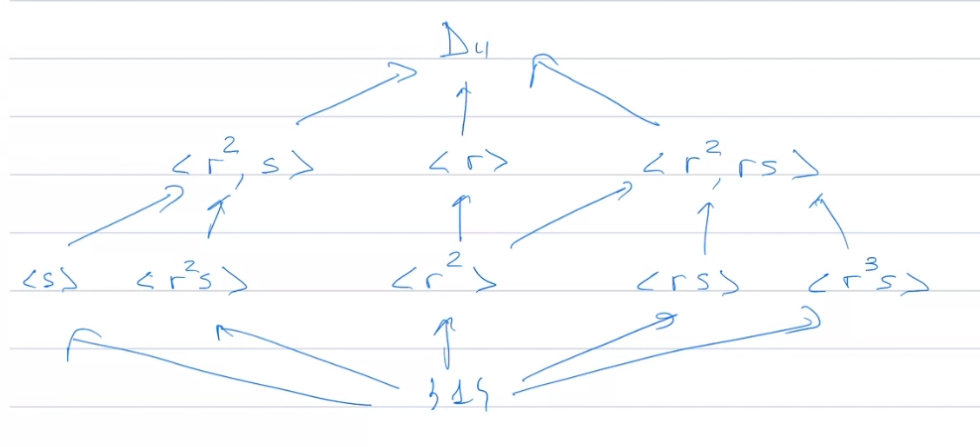
\includegraphics[width=0.75\textwidth]{./Tema5_1}\par\vspace{1cm}
\end{center}

Subgrupos normales son
$$<r^{2},s> \hspace{1cm} <r> \hspace{1cm} <r^{2},rs>$$
pues son de índice dos en $D_{4}$. \\
$Z(D_{4}) = \{1,r^{2}\} = <r^{2}>$ y entonces $<r^{2}> \unlhd D_{4}$ \\
El resto de subgrupos de orden 2 de $D_{4}$ no son normales en $D_{4}$
$$<s> = \{1, s\} \hspace{1cm} r \in D_{4}$$
$$rsr^{-1} = rsr^{3} = rr^{-3}s = r^{-2}s = r^{2}s \notin <s>$$
Por tanto
$$r<s>r^{-1} \nleq <s> \Rightarrow <s> \ntrianglelefteq D_{4}$$
De igual forma para los otros tres:
$$<r^{2},s> \underset{\neq}{\unlhd}  D_{4}$$
$$<r> \underset{\neq}{\unlhd}  D_{4}$$
$$<r^{2},rs> \underset{\neq}{\unlhd}  D_{4}$$

$$1 \underset{\neq}{\unlhd}  <s> \underset{\neq}{\unlhd}  <r^{2},s> \underset{\neq}{\unlhd}  D_{4}$$
$$1 \underset{\neq}{\unlhd}  <r^{2}> \underset{\neq}{\unlhd}  <r^{2},s> \underset{\neq}{\unlhd}  D_{4}$$
$$1 \underset{\neq}{\unlhd}  <r^{3}s> \underset{\neq}{\unlhd}  <r^{2},s> \underset{\neq}{\unlhd}  D_{4}$$
$$1 \underset{\neq}{\unlhd}  <r^{2}s> \underset{\neq}{\unlhd}  <r> \underset{\neq}{\unlhd}  D_{4}$$
$$1 \underset{\neq}{\unlhd}  <r^{2}> \underset{\neq}{\unlhd}  <r^{2},rs> \underset{\neq}{\unlhd}  D_{4}$$
$$1 \underset{\neq}{\unlhd}  <rs> \underset{\neq}{\unlhd}  <r^{2},rs> \underset{\neq}{\unlhd}  D_{4}$$
$$1 \underset{\neq}{\unlhd}  <r^{3}s> \underset{\neq}{\unlhd}  <r^{2},rs> \underset{\neq}{\unlhd}  D_{4}$$

Factores de la 1ª serie son:
$$\sfrac{D_{4}}{<r^{2},s>} \cong C_{2} \hspace{1cm} \sfrac{<r^{2},s>}{<s>} \cong C_{2} \hspace{1cm} \sfrac{<s>}{1} = <s> \cong C_{2}$$

De forma análoga, se observa que los elementos de las demás series son, salvo isomorfismo, $C_{2}$.

\subsection*{Definición}

Sea $G$ un grupo y
$$1 = H_{0} \unlhd H_{1} \unlhd ... \unlhd H_{n} = G$$
$$1 = K_{0} \unlhd K_{1} \unlhd ... \unlhd K_{m} = G$$
dos series normadas de $G$. Diremos que son equivalentes o isomorfas si
\begin{enumerate}[label = (\roman*)]
\item $n = m$
\item $\exists \sigma \in S_{n}$ tal que $\sfrac{H_{i}}{H_{i-1}} \cong \sfrac{K_{\sigma(i)}}{K_{\sigma(i)-1}} \hspace{0.2cm} \forall i = 1, ..., n$.
\end{enumerate}

\subsubsection*{Teorema de Jordan-Holder}

Sea $G$ un grupo que admite una serie de composición. Entonces:
\begin{enumerate}[label = \alph*)]
\item Toda serie normal de $G$ admite un refinamiento que es una serie de composición.
\item Cualesquiera dos series de composición de $G$ son equivalentes.
\end{enumerate}

\subsubsection*{Lema (Teorema de refinamiento de Schreier)}

Cualesquiera dos series normales de un grupo $G$ admiten refinamientos equivalentes.

\subsubsection*{Lema}

Si una serie normal de un grupo $G$ es equivalente a una serie de composición de $G$, entonces dicha serie es también de composición.

\subsubsection*{Demostración (Teorema de Jorda-Holder)}

Sea
$$1 = G_{0} \underset{\neq}{\unlhd} G_{1} \underset{\neq}{\unlhd} ... \underset{\neq}{\unlhd} G_{n} = G$$
una serie de composición de $G$.

\begin{enumerate}[label = \alph*)]
\item Sea $1 = H_{0} \underset{\neq}{\unlhd} H_{1} \underset{\neq}{\unlhd} ... \underset{\neq}{\unlhd} H_{r} = G$ una serie normal de $G$. \\
Por el Teorema de refinamiento de Schreier, ambas series admiten refinamientos equivalentes. \\
Como la serie primera es de composición, todo refinamiento suyo coincide con ella misma. Entonces la serie
$$1 = H_{0} \underset{\neq}{\unlhd} H_{1} \underset{\neq}{\unlhd} ... \underset{\neq}{\unlhd} H_{r} = G$$
tiene un refinamiento equivalente a una serie de composición y entonces, por el segundo lema, dicho refinamiento es también una serie de composición de $G$.
\item Es consecuencia inmediata del Teorema de refinamiento de Schreier.
\end{enumerate}

\subsubsection*{Definición}

Sea $G$ un grupo finito. Definimos la longitud de $G$, que denotaremos por $l(G)$, como la longitud de cualquiera de sus series de composición.

Definimos los factores de composición de $G$ como los factores de sus series de composición. Al conjunto de dichos factores lo denotaremos por $fact(G)$.

\subsubsection*{Ejemplos}

\begin{enumerate}
\item $G = S_{2} \cong C_{2}$. \\
$1 \underset{\neq}{\unlhd} S_{2}$ es una serie de composición de $S_{2}$. \\
Entonces:
$$l(S_{2}) = 1 \hspace{1cm} fact(S_{2}) = \{C_{2}\}$$
\item $S_{3}$ \\
$1 \underset{\neq}{\unlhd} A_{3} \underset{\neq}{\unlhd} S_{3}$ es una serie de composición de $S_{3}$ pues: \\
$\begin{cases}
\sfrac{S_{3}}{A_{3}} \cong C_{2} \\
\sfrac{A_{3}}{1} = A_{3} \cong C_{3}
\end{cases}$ \\
Entonces $l(S_{3}) = 2 \hspace{1cm} fact(S_{3} = \{C_{2}, C_{3}\}$.
\item $S_{4}$ \\
$1 \unlhd C_{2} \underset{\neq}{\unlhd} K \underset{\neq}{\unlhd} A_{4} \underset{\neq}{\unlhd} S_{4}$ serie de composición.
$$l(S_{4}) = 4$$ $$fact(S_{4}) = \{\sfrac{S_{4}}{A_{4}} \cong C_{2}, \sfrac{A_{4}}{K} \cong C_{3} \sfrac{K}{C_{2}} \cong C_{2}, \sfrac{C_{2}}{1} = C_{2}\}$$
\item $G = D_{3} = \{1, r, r^{2}, s, rs, r^{2}s\}$ \\
$1 \unlhd <r> \unlhd D_{3}$ serie de composición de $D_{3}$
$$l(D_{3}) = 2 \hspace{1cm} fact(D_{3} = \{\sfrac{D_{3}}{<r>} \cong C_{2}, <r> \cong C_{3}\}$$
\item $G = D_{4}$ \\
$1 \underset{\neq}{\unlhd} <s> \underset{\neq}{\unlhd} <r^{2},s> \underset{\neq}{\unlhd} D_{4}$ es una serie de composición.
$$l(D_{4}) = 3$$
$$fact(D_{4}) = \{\sfrac{D_{4}}{<r^{2},s>} \cong C_{2}, \sfrac{<r^{2},s>}{<s>} \cong C_{2}, <s> \cong C_{2}\}$$
\end{enumerate}

\subsubsection*{Relación 4: Ejercicio 12}

Vídeo del 28/04/2021.

% 04/05/2021

\subsubsection*{Proposición}

Sea $G$ un grupo finito y $N$ subgrupo normal propio de $G$. Entonces:
$$l(G) = l(N) + l(\sfrac{G}{N})$$
$$fact(G) = fact(N) \cup fact(\sfrac{G}{N})$$

\subsubsection*{Demostración}

Como $N$ un subgrupo normal propio de $G$, entonces la serie
$$1 \underset{\neq}{\unlhd} N \underset{\neq}{\unlhd} G$$
es una serie normal propia de $G$.

Por el Teorema de Jordan-Hölder se puede refinar hasta una serie de composición de $G$. \\
Sea:
$$1 = K_{0} \underset{\neq}{\unlhd} K_{1} \underset{\neq}{\unlhd} ... \underset{\neq}{\unlhd} K_{r} = N \underset{\neq}{\unlhd} K_{r+1} \underset{\neq}{\unlhd} ... \underset{\neq}{\unlhd} K_{n} = G$$
dicho refinamiento. \\
Entonces:
$$1 = K_{0} \underset{\neq}{\unlhd} ... \underset{\neq}{\unlhd} K_{r} = N \text{ es una serie de composición de } N$$
y
$$1 = \sfrac{K_{r}}{N} \underset{\neq}{\unlhd} \sfrac{K_{r-1}}{N} \underset{\neq}{\unlhd} ... \underset{\neq}{\unlhd} \sfrac{K_{n}}{N} = \sfrac{G}{N}$$
es una serie de composición de $\sfrac{G}{N}$. \\
Entonces se deduce el resultado.

\subsubsection*{Teorema de Abel}

Para cada $n \geq 5$ el grupo $A_{n}$ es un grupo simple.

\subsection*{Demostración}

$n \geq 5$ y sea $N \unlhd A_{n}$, $N \leq 1$. \\
Vamos a demostrar que $N = A_{n}$.

Como $N \neq 1$, elegimos en $N$ un $\alpha \in N, \alpha \notin id$ y que mueve el menor nº de elementos de $\{1, 2, ..., n\} \Rightarrow$ veamos que $\alpha$ es un 3-ciclo, es decir, que mueve exactamente 3 elementos. \\
Supongamos que $\alpha$ no es un 3-ciclo, es decir, que mueve más de 3 elementos.
\begin{enumerate}[label = Caso \arabic*:]
\item $\alpha$ mueve exactamente 4 elementos, entonces $\alpha = (x_{1} \hspace{0.1cm} x_{2})(x_{3} \hspace{0.1cm} x_{4})$ (pues los ciclos de longitud 4 son permutaciones impares). \\
Sea $x_{5} \in \{1, 2, ..., n\}$ tal que $x_{5} \neq x_{i} \hspace{0.1cm} i = 1, 2, 3, 4$ (que podemos hacerlo pues $n \geq 5$) y sea $\beta = (x_{3} \hspace{0.1cm} x_{4} \hspace{0.1cm} x_{5}) \in A_{n}$. \\
Entonces $\beta^{-1}N\beta \leqslant N$ pues $N \unlhd A_{n}$, con lo que $\beta^{-1} \alpha^{-1} \beta \in N$. \\
Entonces $\sigma = \beta^{-1}\alpha^{-1}\beta\alpha \in N$. \\
Resulta que $\sigma$ mueve menos elementos que $\alpha$ en contra de la elección de $\alpha$.
$$\sigma = (x_{3} \hspace{0.1cm} x_{5} \hspace{0.1cm} x_{4}) (x_{1} \hspace{0.1cm} x_{2}) (x_{3} \hspace{0.1cm} x_{4}) = (x_{3} \hspace{0.1cm} x_{4} \hspace{0.1cm} x_{5})$$
\item $\alpha$ mueve 5 o mas elementos. \\
Elegimos $x_{1}, x_{2}, x_{3}, x_{4}, x_{5} \in \{1, ..., n\}$ elementos movidos por $\alpha$ y suponemos que $\alpha(x_{1}) = x_{2}$. \\
Consideramos $\beta = (x_{3} \hspace{0.1cm} x_{4} \hspace{0.1cm} x_{5}) \in A_{n}$, entonces como en el caso anterior.
$$\sigma = \beta^{-1} \alpha^{-1} \beta \alpha \in N$$
Vemos que $\sigma$ mueve menos elementos que $\alpha$, o $\sigma$ deja fijos mas elementos que $\alpha$. \\
En efecto, si $j \in \{1, ..., n\}$ tal que $\alpha(j) = j$ entonces $j \neq x_{i} \hspace{0.1cm} \forall i = 1, ..., 5$ y
$$\sigma(j) = \beta^{-1} \alpha^{-1} \beta \alpha (j) = \beta^{-1} \alpha^{-1} \beta (j) = \beta^{-1} \alpha^{-1} (j) = \beta^{-1}(j) = j$$
Pero además:
$$\sigma(x_{1}) = \beta^{-1} \alpha^{-1} \beta \alpha (x_{1}) = \beta^{-1} \alpha^{-1} \beta(x_{2}) = \beta^{-1} \alpha^{-1} (x_{2}) =$$ $$= \beta^{-1} (x_{1}) = x_{1}$$
Por tanto $\sigma$ mueve menos elementos que $\alpha$ en contradicción con la elección de $\alpha$.
\end{enumerate}
Consecuentemente $\alpha = (x_{1} \hspace{0.1cm} x_{2} \hspace{0.1cm} x_{3}) \in N$. \\
Sea $k \neq x_{i} \hspace{0.1cm} i = 1, 2, 3$ y sea $\gamma = (x_{1} \hspace{0.1cm} x_{2}) (x_{3} \hspace{0.1cm} k) \in A_{n}$. \\
Entonces $\gamma N \gamma^{-1} \leqslant N$ por ser $N \unlhd A_{4}$ y entones $\gamma \alpha^{-1} \gamma^{-1} \in N$. \\
Es fácil ver
$$\sigma \alpha^{-1} \sigma^{-1} = (x_{1} \hspace{0.1cm} x_{2} \hspace{0.1cm} k) \in N$$
Entonces $\{(x_{1} \hspace{0.1cm} x_{2} \hspace{0.1cm} k) \mid k \neq x_{1}, x_{2}\} \subset N$ y aplicando el lema anterior
$$A_{n} = <(x_{1} \hspace{0.1cm} x_{2} \hspace{0.1cm} k) \mid k \neq x_{1}, x_{2}> \leqslant N\Rightarrow A_{n} = N$$

\subsubsection*{Corolario}

Para $n \geq 5$, la longitud de $S_{n}$ es 2 y $fact(S_{n}) = \{A_{n}, C_{2}\}$.

\subsubsection*{Demostración}

Por el teorema de Abel, la serie
$$1 \underset{\neq}{\unlhd} A_{n} \underset{\neq}{\unlhd} S_{n}$$
es una serie de composición de $S_{n}$ pues sus factores son $\sfrac{S_{n}}{A_{n}} \cong C_{2}$ y $\sfrac{A_{n}}{1} = A_{n}$ y por tanto simples. \\
Entonces:
$$l(S_{n}) = 2 \hspace{1cm} fact(S_{n}) = \{A_{n}, C_{2}\}$$

\subsubsection*{Lema}

Sea $n \geq 3$ y $x_{1}, x_{2} \in \{1,2,...,n\}$ con $x_{1} \neq x_{2}$. \\
Entonces:
$$A_{n} = <(x_{1} \hspace{0.1cm} x_{2} \hspace{0.1cm} k) \mid k \neq x_{1} \hspace{0.2cm} i=1,2>$$

\subsubsection*{Demostración}

Sabemos que $A_{n}$ está generado por todos los ciclos de longitud 3. \\
Sea:
$$H = <(x_{1} \hspace{0.1cm} x_{2} \hspace{0.1cm} k \mid k \neq x_{1}, x_{2}> \leqslant A_{n}$$
Demostraremos que para cualquier $(i \hspace{0.1cm} j \hspace{0.1cm} k)$ 3-ciclo se verifica que $(i \hspace{0.1cm} j \hspace{0.1cm} k) \in H$.

Como
$$(x_{1} \hspace{0.1cm} x_{2} \hspace{0.1cm} k) = (x_{2} \hspace{0.1cm} k \hspace{0.1cm} x_{1}) = (k \hspace{0.1cm} x_{1} \hspace{0.1cm} x_{2}) \in H$$
Como $(x_{1} \hspace{0.1cm} x_{2} \hspace{0.1cm} k)^{-1} = (k \hspace{0.1cm} x_{2} \hspace{0.1cm} x_{1}) \in H$
$$(x_{1} \hspace{0.1cm} k \hspace{0.1cm} x_{2}) = (k \hspace{0.1cm} x_{2} \hspace{0.1cm} x_{1}) \in H$$

Sea $\alpha = (i \hspace{0.1cm} j \hspace{0.1cm} k)$ un 3-ciclo.
\begin{enumerate}[label = Caso \arabic*:]
\item $\{x_{1}, x_{2}\} \leqslant \{i, j, k\} \Rightarrow$ por la observación anterior, $(i \hspace{0.1cm} j \hspace{0.1cm} k) \in H$.
\item $x_{1} \in \{i, j, k\} \wedge x_{2} \notin \{i, j, k\}$. \\
Si $i = x_{1}$ entones: \\
$a) \alpha = (x_{1} \hspace{0.1cm} j \hspace{0.1cm} k) = (x_{1} \hspace{0.1cm} x_{2} \hspace{0.1cm} k)^{-1}(x_{1} \hspace{0.1cm} x_{2} \hspace{0.1cm} j)(x_{1} \hspace{0.1cm} x_{2} \hspace{0.1cm} k) \in H$ \\
Si $j = x_{1}$ entonces \\
$b) \alpha = (i \hspace{0.1cm} x_{1} \hspace{0.1cm} k) = (x_{1} \hspace{0.1cm} k \hspace{0.1cm} i) \in H$ por el caso anterior $a)$. \\
Si $k = x_{1}$ entonces \\
$c) \alpha = (i \hspace{0.1cm} j \hspace{0.1cm} x_{1}) = (x_{1} \hspace{0.1cm} i \hspace{0.1cm} j) \in H$ por el primer caso $a)$.
\item $x_{i} \notin \{i, j, k\} \wedge x_{2} \in \{i,j,k\}$ \\
Se procede de forma análoga al caso 2 y se concluye entonces $\alpha \in H$.
\item $x_{1}, x_{2} \notin \{i, j, k\}$.
$$\alpha = (i \hspace{0.1cm} j \hspace{0.1cm} k) = (x_{1} \hspace{0.1cm} x_{2} \hspace{0.1cm} i) (x_{2} \hspace{0.1cm} j \hspace{0.1cm} k) (x_{1} \hspace{0.1cm} x_{2} \hspace{0.1cm} i)^{-1} \in H$$
Por tanto $H$ contiene todos los 3-ciclos y entonces $H = A_{n}$.
\end{enumerate}

% 05/05/2021

\subsection{Grupos resolubles}

\subsubsection*{Definición}

Un grupo $G$ se dice resoluble si tiene una serie normal
$$1 = H_{0} \unlhd H_{1} \unlhd ... \unlhd H_{n} = G$$
tal que $\sfrac{H_{i}}{H_{i-1}}$ es abeliano $\forall i = 1, ...., n$.

Es claro que si $G$ es un grupo abeliano entonces $G$ es resoluble pues la serie
$$1 \unlhd H_{0} \unlhd H_{1} = G$$
tiene sus factores abelianos ($\sfrac{H_{1}}{H_{0}} = G$).

\subsubsection*{Teorema}

Sea $G$ un grupo finito. Son equivalentes los siguientes enunciados:
\begin{enumerate}[label = (\roman*)]
\item Los factores de composición de $G$ son cíclicos de orden un número primo.
\item $G$ es resoluble.
\end{enumerate}

\subsubsection*{Demostración}

\begin{enumerate*}
\item[$(\romannum{1}) \Rightarrow (\romannum{2})$] Es inmediato.
\item[$(\romannum{2}) \Rightarrow (\romannum{1})$] Suponemos $G$ resoluble, sea
$$1 = G_{0} \unlhd G_{1} \unlhd ... \unlhd G_{n} = G$$
serie normal de $G$ con $\sfrac{G_{i}}{G_{i-1}}$ abeliano $\forall i = 1,..., n$. \\
Como $G$ es finito, podemos aplicar el Teorema de Jordan-Hölder, la serie anterior puede refinarse a una serie de composición de $G$. \\
Sea $1 = H_{0} \underset{\neq}{\unlhd} H_{1} \underset{\neq}{\unlhd} ... \underset{\neq}{\unlhd} H_{m} = G$ serie de composición de $G$ que refina a la anterior.

Veamos que $\sfrac{H_{r}}{H_{r-1}}$ es abelaino $\forall r = 1, ..., m$. Elegimos un $r$, y existirá un $i \in \{1, ..., n\}$ tal que $H_{r} \leqslant G_{i}$ (usando que la serie de composición es un refinamiento)
\begin{enumerate}[label = Caso \arabic*:]
\item $H_{r-1} = G_{i-1}$ entonces
$$\sfrac{H_{r}}{H_{r-1}} = \sfrac{H_{r}}{G_{i-1}} \leqslant \sfrac{G_{i}}{G_{i-1}} \text{ que es abeliano}$$
$$\Rightarrow \sfrac{H_{r}}{H_{r-1}} \text{ también es abeliano}$$
\item $H_{r-1} \neq G_{i-1}$ entonces
$$G_{i-1} \unlhd H_{r-1} \underset{\neq}{\unlhd} H_{r} \leqslant G_{i}$$
Entonces
$$\sfrac{H_{r}}{H_{r-1}} \overset{\text{2º Teorema de Isomorfia}}{\cong} \sfrac{\sfrac{H_{r}}{G_{i-1}}}{\sfrac{H_{r-1}}{G_{i-1}}}$$
es abeliano porque $\sfrac{H_{r}}{G_{i-1}}, \sfrac{H_{r-1}}{G_{i-1}}$ son subgrupos de $\sfrac{G_{i}}{G_{i-1}}$ que es abeliano.

Como $\sfrac{H_{r}}{H_{r-1}}$ es simple y abeliano $\Rightarrow \sfrac{H_{r}}{H_{r-1}}$ es cíclico de orden primo $\forall r = 1, ..., m$.
\end{enumerate}
\end{enumerate*}

\subsubsection*{Corolario}

$S_{n}$ es resoluble $\iff n \leq 4$.

\subsubsection*{Demostración}

\begin{enumerate*}
\item[$\Leftarrow)$] Si $n \leq 4 \Rightarrow n=2, 3$ ó $4$. \\
$\begin{cases}
fact(S_{2}) = \{C_{2}\} \\
fact(S_{3}) = \{C_{2}, C_{3}\} \\
fact(S_{4}) = \{C_{2}, C_{2}, C_{2}, C_{3}\}
\end{cases}
\Rightarrow$ son resolubles por el teorema anterior.
\item[$\Rightarrow)$] Si $n \geq 5$ entonces $fact(S_{n}) = \{C_{2}, A_{n}\}$. \\
Como $A_{n}$ no es cíclico de orden primo entonces $S_{n}$ no es resoluble por el Teorema anterior.
\end{enumerate*}

\subsubsection*{Ejemplo}

Hemos visto que:
$$fact(D_{3}) = \{C_{2}, C_{3}\}$$
$$fact(D_{4}) = \{C_{2}, C_{2}, C_{2}\}$$
$$fact(D_{6}) = \{C_{3}, c_{2}, C_{2}\}$$
entonces $D_{3}, D_{4}$ y $D_{6}$ son resolubles.

\subsubsection*{Proposición}

\begin{enumerate}[label = \arabic*)]
\item Sea $G$ un grupo resoluble y $H \leqslant G$, entonces $H$ es resoluble.
\item Sea $G$ un grupo resoluble y $N \unlhd G$ entonces $\sfrac{G}{N}$ es resoluble.
\item Sea $G$ un grupo y $N \unlhd G$ tal que $N$ y $\sfrac{G}{N}$ son resolubles, entonces $G$ es resoluble.
\end{enumerate}

\subsubsection*{Demostración}

Haremos uso de los siguientes resultados (Ejercicio).

\begin{enumerate}[label = (\alph*)]
\item Sean $N, N', H \leqslant G$ con $N \unlhd N' \Rightarrow N \cap H \unlhd N' \cap H$.
\item $H, H', N \leqslant G$ con
$\begin{cases}
H \unlhd H' \\
N \unlhd G
\end{cases}
\Rightarrow NH \unlhd NH'$
\end{enumerate}

\begin{enumerate}[label = \arabic*)]
\item Sea $1 = G_{0} \unlhd G_{1} \unlhd ... \unlhd G_{n} = G$ serie normal de $G$ con $\sfrac{G_{i}}{G_{i-1}}$ abeliano, $i = 1, ..., n$. \\
Sea $H \leqslant G$. Por $(a)$, obtenemos una serie normal
$$1 = G_{0} \cap H \unlhd G_{1} \cap H \unlhd ... \unlhd G_{n} \cap H = G \cap H = H$$
de $H$. \\
Sea $i \in \{1, ..., n\}$, aplicamos el 3º Teorema de isomorfia a $G_{i}$ y a los subgrupos
$$K = G_{i} \cap H \leqslant G_{i}$$
$$N = G_{i-1} \unlhd G$$
Entonces $\sfrac{K}{N \cap K} \cong \sfrac{KN}{N}$, es decir
$$\sfrac{G_{i} \cap H}{G_{i-1} \cap H} = \sfrac{G_{i} \cap H}{G_{i-1} \cap G_{i} \cap H} \cong \sfrac{G_{i-1}(G_{i} \cap H)}{G_{i-1}}$$
Puesto que $\sfrac{G_{i-1}(G_{i} \cap H)}{G_{i-1}} \leqslant \sfrac{G_{i}}{G_{i-1}}$ y entonces abeliano.

Consecuentemente $H$ tiene una serie normal con factores abelianos. Es decir, $H$ es resoluble.
\item $N \unlhd G, G$ resoluble. \\
Sea $1 = G_{0} \unlhd G_{1} \unlhd ... \unlhd G_{n} = G$ serie normal de $G$ con $\sfrac{G_{i}}{G_{i-1}}$ abeliano, $i = 1, ..., n$.

Por $(b)$, $G_{i-1}N \unlhd G_{i} N \hspace{0.2cm} \forall i = 1, ..., n$. \\
Además $N$ es normal en todo $G_{i}N$ pues $N$ es normal en $G$ y entonces, tomando cociente
$$1 = \sfrac{G_{0}N}{N} \unlhd \sfrac{G_{1}N}{N} \unlhd ... \unlhd \sfrac{G_{n}N}{N} = \sfrac{GN}{N} = \sfrac{G}{N}$$
es una serie normal de $\sfrac{G}{N}$. Sus factores $i = 1, ..., n$
$$\sfrac{\sfrac{G_{i}N}{N}}{\sfrac{G_{i-1}N}{N}} \overset{\text{2º Teorema de Isomorfia}}{\cong} \sfrac{G_{i}N}{G_{i-1}N}$$

Aplicamos el tercer teorema de isomorfia a \\
$K \hspace{1cm} G_{i} \unlhd G_{i}N$ \\
$N \hspace{0.9cm}G_{i-1}N \unlhd G_{i}N$
$$\sfrac{G_{i}}{(G_{i-1}N) \cap G_{i}} \cong \sfrac{G_{i}(G_{i-1}N)}{G_{i-1}N} = \sfrac{G_{i}N}{G_{i-1}N}$$
$$\sfrac{G_{i}}{(G_{i-1}N) \cap G_{i}} \overset{\text{2º Teorema de Isomorfia}}{\cong} \sfrac{\sfrac{G_{i}}{G_{i-1}}}{\sfrac{(G_{i-1})N) \cap G_{i}}{G_{i-1}}}$$
y por tanto abeliano al ser cociente de $\sfrac{G_{i}}{G_{i-1}}$ que es abeliano.

Consecuentemente $\sfrac{G}{N}$ tiene una serie normal con factores abelianos. Es decir, $\sfrac{G}{N}$ es resoluble.
\item $N \unlhd G$, $N$ y $\sfrac{G}{N}$ resolubles. \\
Sean $1 = N_{0} \unlhd N_{1} \unlhd ... \unlhd N_{r} = N$ serie normal de $N$ tal que $\sfrac{N_{i}}{N_{i-1}}$ es abeliano $\forall i = 1, ..., r$. \\
Sean
$$1 = \sfrac{N}{N} \unlhd \sfrac{H_{1}}{N} \unlhd ... \unlhd \sfrac{H_{s}}{N} = \sfrac{G}{N}$$
serie normal de $\sfrac{G}{N}$ tal que $\sfrac{\sfrac{H_{j}}{N}}{\sfrac{H_{j-1}}{N}} \cong \sfrac{H_{j}}{H_{j-1}}$ es abeliano $\forall j = 1, ..., s$.

Entonces es inmediato que
$$1 = N_{0} \unlhd N_{1} \unlhd ... \unlhd N_{r} = N \unlhd H_{1} \unlhd ... \unlhd H_{s} = G$$
es una serie normal cuyos factores son abelianos. Por tanto $G$ es resoluble.
\end{enumerate}

\subsubsection*{Corolario}

Para todo $n \geq 3$, el grupo diédrico $D_{n}$ es resoluble.

\subsubsection*{Demostración}

$D_{n} = <r,s \mid r^{n} = 1 = s^{2}, sr = r^{-1}s>$ \\
Consideramos $N = <r> \cong G_{n}$. \\
$N \unlhd D_{n}$ pues $[D_{n} : N] = 2$.

$N$ es abeliano y entonces resoluble. $\sfrac{D_{n}}{N} \cong C_{2}$ abeliano y entonces resoluble $\Rightarrow D_{n}$ es resoluble.

\subsection{Conmutadores}

\subsubsection*{Definición}

Sea $G$ un grupo y sean $x_{1}y \in G$. Definimos el conmutador de $x$ e $y$, denotado $[x,y]$, como el elemento:
$$[x.y] := xyx^{-1}y^{-1}$$
Definimos el subgrupo conmutador (ó también llamado primer subgrupo derivado) de $G$, denotado por $[G, G]$, como el subgrupo generado por los conmutadores. Esto es:
$$[G, G] := <[x,y] \mid x,y \in G>$$

\subsubsection*{Proposición}

Sea $G$ un grupo. Entonces:
\begin{enumerate}[label = (\arabic*)]
\item $[G, G] \unlhd G$:
\item $[G, G] = 1 \iff G$ es abeliano,
\item $\sfrac{G}{[G,G]}$ es un grupo abeliano.
\item Si $N \unlhd G$, entonces $\sfrac{G}{N}$ es abeliano $\iff [G,G] \leqslant N$.
\end{enumerate}

Al cociente $\sfrac{G}{[G,G]}$ se le llama el abelianizado de $G$.

\subsubsection*{Demostración}

\begin{enumerate}[label = (\arabic*)]
\item Puesto que $\{[x,y] \mid x,y \in G\}$ generan $[G,G]$, para ver que $[G,G] \unlhd G$ basta ver que $a[x,y]a^{-1} \in [G,G] \forall a \in G$. Esto último es claro porque
$$a[x,y]a^{-1} = [axa^{-1}, aya^{1}] \in [G,G]$$
\item Es inmediato.
\item Sean $x[G,G], y[G,G] \in \sfrac{G}{[G,G]}$.
$$(x[G,G])(y[G,G]) = (xy)[G,G]$$
$$(y[G,G])(x[G,G]) = yx[G,G]$$
Como
$$(yx)^{-1}xy = x^{-1}y^{-1}xy = [x^{-1}, y^{-1}] \in [G,G]$$
$\Rightarrow (xy) [G,G] = yx[G,G]$ y se tiene que $\sfrac{G}{[G,G]}$ es abeliano.
\item $N \unlhd G$. \\
$\sfrac{G}{N}$ es abeliano $\iff \\ \iff (xy)N = (xN) (yN) = (yN) (xN) = (yx) N \hspace{0.2cm} \forall x, y \in G \iff \\ \iff (yx)^{-1} (xy) = x^{-1} y^{-1} xy = [x^{-1}, y^{-1}] \in N \hspace{0.2cm} \forall x, y \in G \iff \\ \iff \{[x,y] \mid x, y \in G\} \subset N$
\end{enumerate}

\subsubsection*{Relación 4: Ejercicio 3}

Vídeo del 05/05/2021.

\subsubsection*{Definición}

Sea $G$ un grupo. Para cada $n \geq 0$ definimos el $n$-ésimo subgrupo derivado de $G$, por recurrencia, como sigue:
$$G^{(0)} := G$$
$$G^{(n+1)} := [G^{(n)}, G^{(n)}] \forall n \geq 0$$

Notemos que tenemos la siguiente serie:
$$... \unlhd G^{(n+1)} \unlhd G^{(n)} \unlhd ... \unlhd G^{(2)} \unlhd G^{(1)} \unlhd G^{(0)} = G$$
que en general no tiene porque ser finita. \\
Sus factores son:
$$\sfrac{G^{(n)}}{G^{(n+1)}} = \sfrac{G^{(n)}}{[G^{(n)},G^{(n)}]} \text{ abelianos}$$
Esta serie se conoce por la serie derivada de $G$.

\subsubsection*{Teorema}

Sea $G$ un grupo. \\
$G$ es resoluble $\iff \exists n$ tal que $G^{(n)} = 1$.

\subsubsection*{Demostración}

\begin{enumerate*}
\item[$\Leftarrow)$] Inmediato.
\item[$\Rightarrow)$] Supongamos $G$ resoluble y sean
$$1 = H_{0} \unlhd H_{1} \unlhd ... \unlhd H_{n} = G$$
serie normal de $G$ con $\sfrac{H_{i}}{H_{i-1}}$ abeliano $\forall i = 1, ..., n$. \\
Veamos que para todo $i \geq 1, G^{(i)} \leqslant H_{n-1}$, por inducción en $i$. \\
Sea $i = 1$. Puesto que:
$\sfrac{G_{n}}{H_{n-1}} = \sfrac{G}{H_{n-1}}$ es abeliano $\Rightarrow [G,G] = G^{(1)} \leqslant H_{n-1}$ y se tiene el resultado para $i = 1$. \\
Supuesto cierto  para $i$, esto es $G^{(i)} \leqslant H_{n-i}$, veamoslo para $i+1$. \\
Puesto que $\sfrac{H_{n-i}}{H_{n-i-1}}$ es abeliano $\Rightarrow [H_{n-i}, H_{n-1}] \leqslant H_{n-(i+1)}$ \\
$G^{(i)} \leqslant H_{n-i} \Rightarrow [G^{(i)}, G^{(i)}] = G^{(i+1)} \leqslant [H_{n-i}, H_{n-i}] \leqslant H_{n-(i+1)}$ \\
tenemos pues $G^{(i+1)} \leqslant H_{n-(i+1)}$. \\
Tomando $i = n$, $G^{(n)} \leqslant H_{n-n} = H_{0} = 1 \Rightarrow G^{(n)} = 1$.
\end{enumerate*}

% 10/05/2021

\subsection{Ejercicios}

\subsubsection*{Relación 4: Ejercicio 2}

Vídeo del 10/05/2021.

\subsubsection*{Relación 4: Ejercicio 4}

Vídeo del 10/05/2021.

\subsubsection*{Relación 4: Ejercicio 6}

Vídeo del 10/05/2021.

\subsubsection*{Ejercicio}

Si $G$ es un grupo y $N \unlhd G$ tal que $N$ y $\sfrac{G}{N}$ son finitos, entonces $G$ es finito.

Vídeo del 10/05/2021.

\subsubsection*{Relación 4: Ejercicio 11}

Vídeo del 10/05/2021.

\subsubsection*{Relación 4: Ejercicio 15}

Vídeo del 10/05/2021.

\newpage

% 11/05/2021

\section{G-conjuntos y p-grupos}

\subsubsection*{Definición}

Sea $G$ un grupo y $X$ un conjunto no vacío. Una acción de $G$ sobre $X$ (por la izquierda) es una aplicación:
$$G \times X \to X \hspace{1cm} (g,x) \mapsto ^{g}x$$
que verifica las dos siguientes propiedades:
\begin{enumerate}[label = \arabic*)]
\item $^{1}x = x \hspace{0.5cm} \forall x \in X$.
\item $^{gh}x = ^{g}(^{h}x) \hspace{0.5cm} \forall g, h \in G \hspace{0.2cm} \forall x \in X$.
\end{enumerate}
Al elemento $^{g}x$ lo leeremos como el resultado de hacer actuar el elemento $g$ sobre el elemento $x$. \\
Diremos que $G$ actúa sobre $X$ (por la izquierda) ó que $X$ es un $G$-conjunto. \\
$G =$ dominio de operadores. \\
A la acción $G \times X \to X$ aplicación $G$-estructura de $X$. \\
Trabajaremos siempre con acciones por la izquierda.

Para cada $g \in G$, podemos definir la siguiente aplicación:
$$\upphi (g): X \to X \hspace{1cm} \upphi (g)(x) := ^{g}x$$
La condición $1)$ nos dice:
$$\upphi(1) = id_{X}: X \to X$$
La condición $2)$ nos dice que, dados $g, h \in G$:
$$\upphi(g,h) = \upphi(g)_{o}\upphi(h)$$
En particular:
$$\upphi(gg^{-1}) = id_{X} = \upphi(g)_{o}\upphi(g^{-1})$$
$$\upphi(g^{-1}g) = id_{X} = \upphi(g^{-1})_{o}\upphi(g)$$
Es decir, $\upphi(g): X \to X$ es biyectiva con $\upphi(g)^{-1} = \upphi(g^{-1})$. Entonces tenemos definido un homomorfismo de grupos:
$$\upphi: G \to S(X) \hspace{1cm} g \mapsto \upphi(g): X \to X \hspace{0.5cm} \upphi(g)(x) = ^{g}x$$
donde $S(X)$ es el grupo de permutaciones del conjunto $X$. \\
Este homomorfismo la llamaremos representación de $G$ por permutaciones asociada a la acción.

Recíprocamente: Sea $G$ un grupo y $X$ un conjunto no vacío. Supongamos dado un homomorfismo:
$$f: G \to S(X)$$
Entonces podemos definir una acción de $G$ sobre $X$ como sigue:
$$G \times X \to X \hspace{1cm} (g, x) \mapsto ^{g}x := f(g)(x)$$
La condición $1)$ se deduce de que $f(1) = id_{X}$. \\
La condición $2)$ se deduce de que $f(gh) = f(g)_{o}f(h)$. \\
Además, es fácil ver que la representación de $G$ es asociada a esta acción es el homomorfismo de $f$.

\subsubsection*{Definición}

Una acción de $G$ sobre un conjunto $X$ diremos que es fiel si el núcleo de $\upphi: G \to S(X)$ es trivial.

$$Ker(\upphi) = \{g \in G \mid \upphi(g) = id_{X}\} = \{g \in G \mid \upphi(g)(x) = x \hspace{0.2cm} \forall x \in X\} =$$ $$= \{g \in G \mid ^{g}x = x \hspace{0.2cm} \forall x \in X\}$$

\subsubsection*{Ejemplos}

\begin{enumerate}[label = \arabic*)]
\item Dado $G$ un grupo y $X \neq \emptyset$. La aplicación
$$G \times X \to X \hspace{1cm} (g,x) \mapsto ^{g}x := x$$
es una acción de $G$ sobre $X$ que llamaremos la acción trivial de $G$ sobre $X$. \\
La representación asociada es el homomorfismo trivial:
$$\upphi: G \to S(X) \hspace{1cm} g \mapsto id_{X} \Leftarrow \upphi(g)(x) = ^{g}x = x \hspace{0.2cm} \forall x \in X$$
$Ker(\upphi) = G$.
\item Supongamos $X$ un $G$-conjunto y $H \leqslant G$ un subgrupo de $G$. Entonces $X$ también es un $H$-conjunto con acción
$$H \times X \to X$$
definida como la de $G \times X \to X$ restringiéndose a los elementos de $H$. \\
Esta acción se llama la acción por restricción. \\
Si $\upphi: G \to S(X)$ es la representación de $G$, entonces la de $H$ no es otra que la composición:
$$H \overset{i}{\hookrightarrow} G \overset{\upphi}{\to} S(X)$$
\item $G = S_{n}$ y $X = \{1,2,...,n\}$. Entonces:
$$S_{n} \times X \to X \hspace{0.5cm} (\sigma, i) \mapsto ^{\sigma}i := \sigma(i)$$
es una acción de $S_{n}$ sobre $X$ cuya representación asociada
$$id_{S_{n}} = \upphi: S_{n} \to S(X) = S_{n}$$
Por tanto se trata de una acción fiel.
\item $G = D_{4} = \{1, r, r^{2}, r^{3}, s, rs, r^{2}s, r^{3}s\}$ y $X = \{1, 2, 3, 4\}$. Sea
$$\upphi: D_{4} \to S(X) = S_{4}$$
$$\upphi(r^{i}) = (1 \hspace{0.1cm} 2 \hspace{0.1cm} 3 \hspace{0.1cm} 4)^{i} \hspace{1cm} 0 \leq i \leq 3$$
$$\upphi(r^{i}s) = (1 \hspace{0.1cm} 2 \hspace{0.1cm} 3 \hspace{0.1cm} 4)^{i} (2 \hspace{0.1cm} 4) \hspace{1cm} 0 \leq i \leq 3$$
$\upphi$ es un homomorfismo de grupos (ejercicio).

Tenemos entonces una acción:
$$D_{4} \times \{1, 2, 3, 4\} \to \{1, 2, 3, 4\}$$
$$g_{j} := \upphi(g)(j) \hspace{1cm} g \in D_{4}, j \in \{1, 2, 3, 4\}$$
$g_{j}$ es precisamente el resultado de aplicar al vértice $j$ el movimiento que corresponde a $g$.
$$r_{j} = \upphi(r)(j) = (1 \hspace{0.1cm} 2 \hspace{0.1cm} 3 \hspace{0.1cm} 4) (j)$$
$Ker(\upphi) = \{1\}$ y entonces es fiel.
\item $G = S_{n} \hspace{1cm} X$ cualquier conjunto, $X \neq \emptyset$. \\
Consideramos $X^{n} = X \times \overset{n}{...} \times X$. \\
Definimos una acción de $S_{n}$ sobre $X^{n}$ como sigue:
$$S_{n} \times X^{n} \to X^{n}$$
$$(\sigma, (x_{1}, x_{2}, ..., x_{n})) \mapsto ^{\sigma} (x_{1}, x_{2}, ..., x_{n}) := (x_{\sigma^{-1}(1)}, x_{\sigma^{-1}(2)}, ..., x_{\sigma^{-1}(n)})$$
Veamos la propiedad 2: \\
$\sigma, \tau \in S_{n}$
$$^{\sigma \tau}(x_{1}, x_{2}, ..., x_{n}) = ^{\sigma}(^{\tau}(x_{1}, x_{2}, ..., x_{n}))$$
$$^{\sigma \tau}(x_{1}, x_{2}, ..., x_{n}) = (x_{(\sigma \tau)^{-1}(1)}, x_{(\sigma \tau)^{-1}(2)}, ..., x_{(\sigma \tau)^{-1}(n)}) =$$ $$= (x_{\tau^{-1}\sigma^{-1}(1)}, x_{\tau^{-1}\sigma^{-1}(2)}, ..., x_{\tau^{-1}\sigma^{-1}(n)})$$
$$^{\tau}(x_{1}, x_{2}, ..., x_{n}) = (x_{\tau^{-1}(1)}, x_{\tau^{-1}(2)}, ..., x_{\tau^{-1}(n)}) = (y_{1}, ..., y_{n})$$
$$y_{j} = x_{\tau^{-1}(j)} \hspace{1cm} j = 1, ..., n$$
$$^{\sigma}(^{\tau}(x_{1}, x_{2}, ..., x_{n})) = ^{\sigma}(y_{1}, y_{2}, ..., y_{n}) = (y_{\sigma^{-1}(1)}, y_{\sigma^{-1}(2)}, ..., y_{\sigma^{-1}(n)})$$
Ahora $y_{\sigma^{-1}(j)} = x_{\tau^{-1}\sigma^{1}(j)} \hspace{0.5cm} \forall j = 1, ..., n$ \\
$= (x_{\tau^{-1}\sigma^{-1}(1)}, x_{\tau^{-1}\sigma^{-1}(2)}, ..., x_{\tau^{-1}\sigma^{-1}(n)})$.

La aplicación:
$$S_{n} \times X^{n} \to X^{n}$$
$$(\sigma, (x_{1}, ..., x_{n})) \to (x_{\sigma(1)}, x_{\sigma(2)}, ..., x_{\sigma(n)})$$
en general no es acción.

% 12/05/2021

\item  Sea $G$ un grupo y $X = G$, entonces podemos definir una acción de $G$ sobre $G$ llamada la acción por traslación y dada como sigue:
$$G \times G \to G \hspace{1cm} (g, h) \mapsto ^{g}(h) := gh$$
Si $\varphi: G \to S(G)$ es la representación asociada.
$$Ker(\upphi) = \{g \in G \mid \upphi(g) = id_{G}\} = \{g \in G \mid \upphi(g)(h) =$$ $$= h \hspace{0.2cm} \forall h \in G\} = \{g \in G \mid ^{g}h = h \hspace{0.2cm} \forall h \in G\} =$$ $$= \{g \in G \mid gh = h \hspace{0.2cm} \forall h \in G \} = \{1\}$$
Es decir, esta acción es fiel. \\
Si $G$ es finito y $|G| = n$, entonces $S(G) \cong S_{n}$ y como
$$\upphi: G \to S(G) \cong S_{n}$$
es un monomorfismo, aplicando el 1º Teorema de isomorfia
$$G \cong Img(\upphi)$$
\item Sea $G$ un grupo y $H \leqslant G$ subgrupo. Entonces
$$G \times \sfrac{G}{H} \to \sfrac{G}{H}$$
$$(g, xH) \mapsto ^{g}(xH) := gxH$$
También
$$G \times \sfrac{H}{G} \to \sfrac{H}{G}$$
$$(g, Hx) \mapsto ^{g}(Hx) := Hxg^{-1}$$
es una acción
\item Sea $G$ un grupo y consideremos $X = G$. Entonces la aplicación:
$$G \times G \to G \hspace{1cm} (g, h) \mapsto ^{g}h := ghg^{-1}$$
es una acción que llamaremos la acción por conjugación de $G$ sobre sí mismo.
$$\upphi: G \to S(G)$$
$$g \mapsto \upphi(g): G \to G$$
$$\upphi(g)(h) = ^{g}h = ghg^{-1}$$
Es decir, $\upphi(g) = \varphi_{g}$ es el automorfismo interno definido por el elemento $g \in G$.
$$Img(\upphi) = Int(G) \leqslant Aut(G)$$
$$Ker(\upphi) = \{g \in G \mid \varphi_{g} = id_{G}\} = \{g \in G \mid \varphi_{g}(h) = h \hspace{0.2cm} \forall h \in G\} =$$ $$=\{g \in G \mid ghg^{-1} = h \hspace{0.2cm} \forall h \in G\} =\{g \in G \mid gh = hg \hspace{0.2cm} \forall h \in G\} = Z(G)$$
\item Sea $G$ un grupo y consideremos el conjunto $X = Sub(G)$. \\
Entonces:
$$G \times Sub(G) \to Sub(G)$$
$$(g, H) \mapsto ^{g}H := gHg^{-1}$$
es una acción.
\end{enumerate}

\subsubsection*{Teorema de Cayley}

Todo grupo finito es isomorfo a un subgrupo de un grupo de permutaciones.

\subsubsection*{Definición}

Sea $G$ un grupo y $X$ un $G$-conjunto y sea
$$G \times X \to X \hspace{1cm} (g, x) \mapsto ^{g}x$$
la acción. \\
Podemos definir en $X$ la siguiente relación binaria, denotada por $\sim$: \\
Dados $x, y \in X$
$$x \sim y \overset{def}{\iff} \exists g \in G \text{ tal que } y = ^{g}x$$
Esta relación binaria es una relación de equivalencia. \\
En efecto:
\begin{enumerate*}
\item[Simétrica] Supongamos que $x \sim y \Rightarrow \exists g \in G$ tal que $y = ^{g}x$
$$y = ^{g}x \Rightarrow ^{g^{-1}}(y) = ^{g^{-1}}(^{g}x) \underset{2)}{=} ^{(g^{-1}g)}x = ^{1}x \underset{1)}{=} x \Rightarrow y \sim x$$
\end{enumerate*}
De la misma forma se demuestran la propiedad reflexiva y transitiva.

\subsubsection*{Definición}

Para cada $x \in X$, definimos la órbita de $x$, que denotaremos por $\theta(x)$, como la clase de equivalencia de $x$ por la relación de equivalencia anterior. \\
Entonces
$$\theta(x) = \{y \in X \mid x \sim y\} = \{y \in X \mid y = ^{g}x \text{ para } g \in G\} = \{^{g}x \mid g \in G\}$$
Tenemos que
\begin{enumerate}[label = \arabic*)]
\item $\theta(x) = \theta(y) \iff x \sim y \iff \exists g \in G$ tal que $y = ^{g}x$.
\item $\theta(x) \neq \theta(y) \iff \theta(x) \cap \theta(y) = \emptyset$.
\item El conjunto de todas las órbitas, es decir, $\sfrac{X}{\sim}$, es una partición de $X$.
$$X = \cup_{x \in X} \theta(x) \text{ unión disjunta}$$
\end{enumerate}

Una acción diremos que es transitiva si tiene una única órbita (si $\sfrac{X}{\sim}$ es unitario. Es decir,
$$\theta(x) = \theta(y) \hspace{1cm} \forall x, y \in X$$
o, en otros términos, si
$$\forall x, y \in X \hspace{0.5cm} \exists g \in G \text{ tal que } y = ^{g}x$$

\subsubsection*{Definición}

Sea $G$ un grupo y $X$ un $G$-conjunto. Para cada $x \in X$ definimos el estabilizador de $x$ en $G$ como:
$$Stab_{G}(x) := \{g \in G \mid ^{g}x = x\}$$
Se verifica que $Stab_{G}(x)$ es un subgrupo de $G$ (ejercicio). También llamado el grupo de isotropia de $x$ en $G$.

\subsubsection*{Proposición}

Sea $G$ un grupo y $X$ un $G$-conjunto. Sean $x, y \in X$, entonces
$$\theta(x) = \theta(y) \iff Stab_{G}(x), Stab_{G}(y) \text{ son subgrupos conjugados de } G$$
$(H, K \leqslant G, H$ y $K$ se dicen conjugados si $\exists g \in G$ tal que $H = gkg^{-1}$)

\subsubsection*{Demostración}

Suponemos que $\theta(x) = \theta(y) \Rightarrow x \sim y \Rightarrow \exists g \in G$ tal que $y = ^{g}x \Rightarrow ^{g^{-1}}y= x$. \\
Veamos que $g Stab_{G}(x) g^{-1} = Stab_{G}(y)$.

Lo vemos por doble inclusión. \\
Sea $h \in Stab_{G}(x) \Rightarrow ^{h}x = x$. \\
Consideramos $ghg^{-1}$ y lo hacemos actuar sobre $y$
$$^{(ghg^{-1})}y = ^{gh}(^{g^{-1}}y) = ^{(gh)}x = ^{g}(^{h}x) = ^{g}x = y$$
$$\Rightarrow ghg^{-1} \in Stab_{G}(y)$$
Tenemos que $gStab_{G}(x)g^{-1} \leqslant Stab_{G}(y)$. \\
Por el mismo razonamiento anterior y puesto que $x = ^{g^{-1}}y$, tendremos que:
$$g^{-1} Stab_{G}(y)g \leqslant Stab_{G}(x) \Rightarrow Stab_{G}(y) \leqslant gStab_{G}(x) g^{-1}$$
Consecuentemente:
$$Stab_{G}(y) = g Stab(x) g^{-1}$$

\subsubsection*{Teorema}

Sea $G$ un grupo finito y $X$ un $G$-conjunto. Entonces, para cada $x \in X$, la órbita de $x$ es un conjunto finito, teniéndose que
$$|\theta(x)| = [G:Stab_{G}(x)]$$
En particular $|\theta(x)|$ es un divisor de $|G|$.

\subsubsection*{Demostración}

$$\{g Stab_{G}(x) \mid g \in G\} = \sfrac{G}{Stab_{G}(x)} \overset{\lambda}{\to} \theta(x) = \{^{g}x \mid g \in G\}$$
Definimos $\lambda(g Stab_{G}(x)) := ^{g}x$.
$$g Stab_{G}(x) = h Stab_{G}(x) \iff h^{-1}g \in Stab_{G}(x) \iff ^{(h^{-1}g}x = x \iff$$ $$\iff ^{g}x = ^{h}x$$
Por tanto $\lambda$ está bien definida y además $\lambda$ es inyectiva. \\
Obviamente, por definición, $\lambda$ es sobreyectiva.

Por tanto $\lambda$ es biyectiva. \\
Como $\sfrac{G}{Stab_{G}(x)}$ es finito por ser $G$ finito, entonces $\theta(x)$ es finito y
$$|\theta(x)| = [G : Stab_{G}(x)]$$

\subsubsection*{Relación 6: Ejercicio 1}

Vídeo del 12/05/2021.

\subsubsection*{Definición}

Sea $G$ un grupo y $X$ un $G$-conjunto. Un elemento $x \in X$ diremos que es un elemento fijo por la acción si $^{g}x = x \hspace{0.2cm} \forall g \in G$. El conjunto de los elementos fijos lo denotaremos por $Fix(X)$
$$Fix(X) = \{x \in X \mid ^{g}x = x \hspace{0.2cm} \forall g \in G\}$$

Notemos que
$$x \in Fix(X) \iff \theta(x) = \{x\} \iff Stab_{G}(x) = G$$.

Sea $G$ un grupo finito y $X$ un $G$-conjunto finito. El conjunto $\sfrac{X}{\sim}$ también es finito. Supongamos:
$$\sfrac{X}{\sim} = \{\theta(x_{1}), \theta(x_{2}), ..., \theta(x_{r})\}$$
Sabemos que $X = \cup_{i = i}^{r} \theta(x_{i})$ unión disjunta $\Rightarrow$
$$|X| = \sum_{i=1}^{r} |\theta(x_{i})| = |Fix(X)| + \sum_{x \notin Fix(X)} |\theta(x_{i})| =$$ $$= |Fix(X)| + \sum_{x_{i} \notin Fix(X)} [G : Stab_{G}(x_{i})]$$

\subsubsection*{Ejemplo}

\begin{enumerate}[label = \arabic*)]
\item Sea $G$ un grupo cualquiera y consideramos la acción de $G$ sobre sí mismo por traslación
$$G \times G \to G \hspace{1cm} ^{g}h := gh$$
Sea $h \in G$
$$\theta (h) = \{^{g}h \mid g \in G\} = \{gh \mid g \in G\} = G$$
Por tanto $\forall h, h' \in G$, se tiene que $\theta(h) = \theta(h')$, es decir, esta acción es transitiva.
$$Stab_{G}(h) = \{g \in G \mid ^{g}h = h\} = \{g \in G \mid gh = h\} = \{1\}$$
$$Fix(G) = \{h \in G \mid ^{g}h = h \hspace{0.2cm} \forall g \in G\} = \{h \in G \mid gh = h \hspace{0.2cm} \forall g \in G\} = \emptyset$$
\item Sea $G$ un grupo y consideramos la acción de $G$ sobre sí mismo por conjugación
$$G \times G \to G \hspace{1cm} ^{g}h = ghg^{-1}$$
$h \in G$
$$\theta(h) = \{^{g}h \mid g \in G\} = \{ghg^{-1} \mid g \in G\}$$
se llama la clase de conjugación del elemento $h$ en $G$ y se denota por $cl(h)$.
$$Stab_{G}(h) = \{g \in G \mid ^{g}h = h\} = \{g \in G \mid ghg^{-1} = h\} =$$ $$= \{g \in G \mid gh = hg\} \leqslant G$$
se llama el centralizador de $h$ en $G$ y se denota por $c_{G}(h)$.
$$Fix(G) = \{h \in G \mid ^{g}h = h \hspace{0.2cm} \forall g \in G\}  =$$ $$= \{h \in G \mid ghg^{-1} = h \hspace{0.2cm} \forall g \in G\} = \{h \in G \mid gh = hg \hspace{0.2cm} \forall g \in G\} = Z(G)$$
Supongamos que $G$ es un grupo finito.
$$\sfrac{G}{\sim} = \{cl(h_{1}), cl(h_{2}), ..., cl(h_{r})\}$$
Entonces
$$|G| = |Z(G)| + \sum_{h_{i} \notin Z(G)} |cl(h_{i})| = |Z(G)| + \sum_{h_{i} \notin Z(G)} [G:c_{g}(h_{i})]$$
(Fórmula de las clases)
\end{enumerate}

\subsubsection*{Relación 6: Ejercicio 9}

Vídeo del 12/05/2021.

% 17/05/2021

\subsubsection*{Relación 6: Ejercicio 7}

Vídeo del 17/05/2021.

\subsubsection*{Definición}

Sea $p$ un número primo. Un grupo finito $G$ no trivial diremos que es un $p$-grupo si todo elemento de $G$ tiene orden una potencia de $p$.

\subsubsection*{Ejemplos}

\begin{enumerate}[label = \arabic*)]
\item Para cada $n \geq 1, C_{p^{n}} = <x \mid m^{p^{n}} = 1>$ es un $p$-grupo. \\
Porque si $a \in C_{p^{n}} \Rightarrow ord(a) \mid |C_{p^{n}}| = p^{n} \Rightarrow ord(a) = p^{k} \hspace{0.2cm} 0 \leq k \leq n$.
\item Para cada $n \geq 2$, el producto directo
$$G = C_{p} \times C_{p} \times \overset{n}{...} \times C_{p}$$
es un $p$-grupo. \\
Si $(x_{1}, ..., x_{n}) \in G$
$$ord((x_{1}, ..., x_{n})) = mcm(ord(x_{1}), ..., ord(x_{n})) = p^{k} \hspace{0.2cm} 0 \leq k \leq 1$$
Así todo elemento de $G$ tiene orden una potencia de $p$.
\item Si $G$ es un grupo con $|G| = p^{n}$ para $n \geq 1$ entonces, razonando como en el ejemplo 1, $G$ es un $p$-grupo.
\end{enumerate}

\subsubsection*{Teorema de Cauchy}

Sea $G$ un grupo finito. Para cada primo $p$ divisor de $G$ existe $x \in G$ tal que $ord(x) = p$ (entonces $\exists H = <x> \leqslant G$ tal que $|H| = p$).

\subsubsection*{Demostración}

Sea $|G| = n$ y $p \mid n$, $p$ número primo. \\
Sea $X$ definido como sigue:
$$X := \{(x_{1}, x_{2}, ..., x_{p}) \in G^{p} \mid x_{1}x_{2}...x_{p} = 1 \Rightarrow x_{1} = (x_{2}...x_{p})^{-1}\}$$
Como $|G| = n \Rightarrow |X| = n^{p-1}$. \\
Consideramos $\sigma = (1 \hspace{0.1cm} 2 \hspace{0.1cm} ... \hspace{0.1cm} p) \in S_{p}$ y $H = <\sigma> = \{1, \sigma, \sigma^{2}, ..., \sigma^{p-1}\}$.
Definimos una acción de $H$ sobre $X$ como sigue:
$$H \times X \to X$$
$$^{\sigma^{0}}(x_{1}, ..., x_{p}) := (x_{1}, ..., x_{p})$$
$$1 \leq j \leq p-1 \hspace{0.5cm} ^{\sigma^{j}}(x_{1}, ..., x_{p}) := (x_{j+1}, ..., x_{p}, x_{1}, ..., x_{j})$$
(Ejercicio: Demostrad que en efecto tenemos una acción) \\
Sea $(x_{1}, ..., x_{p}) \in X$
$$O((x_{1}, ..., x_{p})) = \{^{\sigma^{j}}(x_{1}, ..., x_{p}) \mid 0 \leq j \leq p-1\} =$$ $$= \{(x_{1}, ..., x_{p}), (x_{2}, ..., x_{p}, x_{1}), (x_{3}, ..., x_{p}, x_{1}, x_{2}), ..., (x_{p}, x_{1}, ..., x_{p-1})\}$$
$|O((x_{1}, ..., x_{p}))|$ divide a $|H| = p \Rightarrow |O((x_{1}, ..., x_{p})) = 1$ ó $p$. \\
Los elementos con $|O(x_{1}, ..., x_{p})| = 1$ son precisamente $(x_{1}, ..., x_{p}) \in Fix(X)$. 
$$(x_{1}, ..., x_{p}) \in Fix(X) \iff x_{1} = x_{2} = ... = x_{p}$$
Puesto que $(1, 1, ..., 1) \in Fix(X)$, entonces $Fix(X) \neq \emptyset$. \\
Sabemos
$$|X| = |Fix(X)| + \sum_{(x_{1}, ..., x_{p}) \notin Fix(X)} |O(x_{1}, ..., x_{p})|$$
Si $(x_{1}, ..., x_{p}) \notin Fix(X) \Rightarrow |O(x_{1}, ..., x_{p})| = p$. \\
Sea $r = |Fix(X)|$ y $s = $ nº de elementos $\notin Fix(X)$.
$$n^{p-1} = |x| = r + ps \Rightarrow
\begin{cases}
r = n^{p-1} - ps \\
p \mid n
\end{cases}
\Rightarrow
p \mid r \Rightarrow r \geq 2$$
Decir que $r \geq 2$ significa que $\exists (x, x, ..., x) \in Fix(X)$ y  \\ $(x, x, ..., x) \neq (1, 1, ..., 1) \iff x \neq 1$. \\
Entonces como $(x, x, ..., x) \in X$, por definición de $X$, $x...x = x^{p} = 1 \hspace{0.5cm} x \neq 1$. \\
Concluimos pues $\exists x \in X$ tal que $ord(x) = p$.

\subsubsection*{Corolario}

Sea $G$ un grupo finito no trivial.
$$G \text{ es un } p \text{-grupo} \iff |G| = p^{n} \text{ para algún } n \geq 1$$

\subsubsection*{Demostración}

\begin{enumerate*}
\item[$\Leftarrow$] Ejemplo 3.
\item[$\Rightarrow$] Sea $|G| = m (m \geq 1)$. \\
Sea $a$ un divisor primo de $m \Rightarrow$ por el teorema de Cauchy $\exists x \in G$ tal que $ord(x) = q$. \\
Por otro lado, como $G$ es un $p$-grupo entonces $ord(x) = p^{k} \hspace{0.2cm} k \geq 1$. \\
Consecuentemente:
$$q = p^{k} \Rightarrow k = 1 \text{ y } p = q$$
Si el único divisor primo de $m$ es $p \Rightarrow m = p^{n}$ para algún $n \geq 1$.
\end{enumerate*}

% 18/05/2021

\subsubsection*{Teorema de Burnside}

Sea $G$ un $p$-grupo finito. Entones $|Z(G)| \geq p$. En particular, $Z(G)$ no es trivial.

\subsubsection*{Demostración}

Como $G$ es un $p$-grupo, supongamos que $|G| = p^{n}, n \geq 1$.

Si $G$ es abeliano $\Rightarrow Z(G) = G$ y se tendría el resultado.

Si $G$ no es abeliano, por la fórmula de las clases
$$|Z(G)| = |G| - \sum_{h \notin Z(G)} |cl(h)|$$
Si $h \notin Z(G) \Rightarrow |cl(h)| > 1$ y como $|cl(h)| = [G:c_{G}(h)]$, es decir, $|cl(h)| \mid |G| = p^{n}$, entonces $|cl(h)| = p^{k} \hspace{0.2cm} k > 0$. Consecuentemente, $p$ es un divisor de $\sum_{h \notin Z(G)} |cl(h)|$. Como $p \mid |G|$, obtenemos que:
$$p \mid |Z(G)| \Rightarrow |Z(G)| \geq p$$

\subsubsection*{Corolario}

Sea $p$ un número primo y $G$ un grupo con $|G| = p^{2}$. Entonces $G$ es abeliano.

\subsubsection*{Demostración}

Por el teorema de Burnside, $|Z(G)| \geq p$. Con lo que $|Z(G)| = p$ ó $|Z(G)| = p^{2}$. \\
Supongamos que $|Z(G)| = p$, entonces $\exists a \in G$ tal que $a \notin Z(G)$
$$c_{G}(a) \leqslant G \hspace{1cm} c_{G}(a) = \{g \in G \mid ag = ga\}$$
Es claro que $Z(G) \lneq c_{G}(a) \Rightarrow |c_{G}(a)| = p^{2} \Rightarrow c_{G}(a) = G \Rightarrow a \in Z(G)$ (Contradicción). \\
Por tanto, $Z(G)| = p^{2} = |G| \Rightarrow Z(G) = G \Rightarrow G$ es abeliano.

\subsubsection*{Corolario}

Si $G$ es un $p$-grupo finito entonces $G$ es resoluble.

\subsubsection*{Demostración}

Sea $|G| = p^{n}, n \geq 1$. Hacemos inducción en $n$. \\
Si $n = 1$, es decir, $|G| = p \Rightarrow G \cong C_{p}$ y por tanto resoluble. \\
Sea $n > 1$ y el resultado cierto para todo $p$-grupo de orden menor que $p^{n}$. Si $G$ es abeliano $\Rightarrow G$ es resoluble y lo tendriamos. Supongamos $G$ no abeliano.
$$1 \underset{\neq}{\unlhd} Z(G) \underset{\neq}{\unlhd} G$$
$\Rightarrow |Z(G)| = p^{k} \hspace{1cm} 1 \leq k < n$. \\
Por hipótesis de inducción, $Z(G)$ es resoluble. Por otro lado
$$|\sfrac{G}{Z(G)}| = p^{n-k} \hspace{0.5cm} 1 \leq n-k < n$$
y entonces, por hipótesis de inducción $\sfrac{G}{Z(G)}$ es resoluble.

$\begin{cases}
Z(G) \unlhd G \text{ resoluble} \\
\sfrac{G}{Z(G)} \text{ resoluble}
\end{cases}
\Rightarrow G$ es resoluble.

\subsubsection*{Definición}

Sea $G$ un grupo finito y $p$ un número primo. \\
Un subgrupo $H$ de $G$ que sea $p$-grupo lo llamaremos un $p$-subgrupo de$G$.

\subsubsection*{Observación}

El teorema de Cauchy nos dice que para cada primo $p$ divisor de $|G|$ existe un $H \leqslant G, |H| = p$ y entonces un $p$-subgrupo.

\subsection{Teoremas de Sylow}

\subsubsection*{Primer teorema de Sylow}

Sea $G$ un grupo finito con $|G| = n$. Sea $p$ un número primo divisor de $n$. \\
Entonces para cada potencia $p^{i}$ con $p^{i} \mid n$ existe $H \leqslant G$ tal que $|H| = p^{i}$.

\subsubsection*{Demostración}

Hacemos inducción en $i$. \\
Para $i = 1$, el resultado se sigue del Teorema de Cauchy. \\
Sea $i > 1$ y supongamos el resultado cierto para todo grupo finito con orden divisible por $p^{j}, j < i$. \\
Veamoslo para $i > 1. |G| = n$ y $p^{i} \mid n$ buscamos $H \leqslant G$ tal que $|H| = p^{i}$. \\
Hacemos inducción $|G|$. Como $p^{i} \mid n$ el primer caso es $|G| = p^{i}$ y entonces basta tomar $H = G$. Supongamos que $|G| = n > p^{i}$ y el resultado cierto para todo grupo de orden menor que $n$ y divisible por $p^{i}$.

\begin{enumerate}[label = Caso \arabic*]
\item $\exists K \nleq G$ tal que $p \nmid [G:K]$. \\
Como
$$\begin{cases}
|G| = [G:K] |K| \\
p^{i} \mid |G| \\
p \nmid [G:K]
\end{cases}
\Rightarrow p^{i} \mid |K|$$
$\begin{cases}
p^{i} \mid |K| \\
K \nleq G \Rightarrow |K| < |G| = n
\end{cases}
\underset{\text{por hipótesis de inducción}}{\Rightarrow} \exists H \leqslant K$ tal que $|H| = p^{i}$. Claramente $H \leqslant G$ y se tiene el resultado.
\item Para todo $K \leqslant G, p \mid [G:K]$. \\
Por la fórmula de las clases
$$|Z(G)| = |G| - \sum_{h \notin Z(G)} [G: c_{G}(h)]$$
$p \mid |G|$ y $p \mid \sum	[G:c_{G}(h)] \Rightarrow p \mid |Z(G)|$. \\
Aplicamos el Teorema de Cauchy a $Z(G)$ y entonces $\exists N \leqslant Z(G)$ tal que $|N| = p$. \\
Como $N \leqslant Z(G) \Rightarrow N \unlhd G$ (Ejercicio). \\
Podemos pues considerar $\sfrac{G}{N}$. Como $|N| = p$ y $p^{i} \mid |G| \Rightarrow p^{i-1} \mid |\sfrac{G}{N}|$. \\
Por hipótesis de inducción en la portencia de $p$,
$$\exists L \leqslant \sfrac{G}{N} \text{ tal que } |L| = p^{i-1}$$
$\Rightarrow L = \sfrac{H}{N} \hspace{0.5cm} N \unlhd H \unlhd G$. \\
$|\sfrac{H}{N}| = p^{i-1} \Rightarrow |H| = |\sfrac{H}{N}||N| = p^{i-1}p = p^{i}$.
\end{enumerate}

\subsubsection*{Definición}

Sea $G$ un grupo finito y $p$ un número divisor de $G$. \\
Sea $p^{k}$ la máxima potencia de $p$ que divide a $|G|$ (es decir, $|G| = p^{k}m, \\ mcd(p,m) = 1$). \\
Los $p$-subgrupos de $G$ de orden $p^{k}$ se llaman $p$-subgrupos de Sylow de $G$.

\subsubsection*{Corolario}

Todo grupo $G$ tiene $p$-subgrupos de Sylow, para cada $p$ divisor de $|G|$.

\subsubsection*{Ejemplos}

\begin{enumerate}[label = \arabic*)]
\item $n \geq 2$ y $C_{n} = <x \mid x^{n} = 1>$. \\
Sea $n = p_{1}^{t_{1}}p_{2}^{t_{2}}...p_{k}^{t_{k}}$ la factorización de $n$ en primos. \\
Para cada $1 \leq i \leq k$, los $p_{i}$-subgrupos de Sylow tienen orden $p_{i}^{t_{i}}$. Sólo hay uno que es
$$C_{p_{i}^{t_{i}}} = <x^{s_{i}}>\hspace{1cm} s_{i} = p_{1}^{t_{1}}p_{2}^{t_{2}}...p_{i-1}^{t_{i-1}}p_{i+1}^{t_{i+1}}...p_{k}^{t_{k}}$$
\item $G = A_{4}, |A_{4}| = 12 = 3 \cdot 2^{2}$ \\
Los 3-subgrupos de Sylow de $A_{r}$ tienen orden 3 y entonces cíclicos de orden 3.
$$\mathcal{P}_{1} = <(1 \hspace{0.1cm} 2 \hspace{0.1cm} 3)>, \mathcal{P}_{2} = <(1 \hspace{0.1cm} 2 \hspace{0.1cm} 4)>, \mathcal{P}_{3} <(1 \hspace{0.1cm} 3 \hspace{0.1cm} 4)>, \mathcal{P}_{4} = <(2 \hspace{0.1cm} 3 \hspace{0.1cm} 4)>$$
Los 2-subgrupos de Sylow de $A_{4}$ tienen orden 4 y sólo tiene uno que es
$$K = \{id, (1 \hspace{0.1cm} 2)(3 \hspace{0.1cm} 4), (1 \hspace{0.1cm} 3)(2 \hspace{0.1cm} 4), (1 \hspace{0.1cm} 4)(2 \hspace{0.1cm} 3)\}$$

Si $\mathcal{P}$ es un p-subgrupo de Sylow de $G$
$$|G| = p^{k}m \hspace{0.5cm} mcd(m, p) = 1$$
Entonces $|\mathcal{P}| = p^{k}$ y por tanto $[G:\mathcal{P}] = m \Rightarrow mcd(|\mathcal{P}|, [G:\mathcal{P}]) = 1$.
\end{enumerate}

% 19/05/2021

\subsubsection*{Lema}

Sea $G$ un grupo finito, $p$ un número primo divisor de $|G|$ y $\mathcal{P}$ un $p$-subgrupo de Sylow de $G$. \\
Sea $H \leqslant G$ un $p$-subgrupo de $G$ tal que $H \leqslant N_{G}(\mathcal{P})$, entonces $H \leqslant \mathcal{P}$.

\subsubsection*{Demostración}

$\mathcal{P} \unlhd N_{G}(\mathcal{P}) \hspace{1cm}$ Aplicamos el tercer teorema. \\
$H \leqslant N_{G}(\mathcal{P}) \hspace{1cm}$ de isomorfía y entonces:

$$\sfrac{H}{H \cap \mathcal{P}} \cong \sfrac{H\mathcal{P}}{\mathcal{P}}$$

Con lo que $r = [H : H \cap \mathcal{P}] = [H\mathcal{P} : \mathcal{P}]$.
$$r \mid |H| \overset{H \text{es un p-grupo}}{\Rightarrow} r = p^{t} \hspace{0.5cm} t \geq 0$$
Consideramos $\mathcal{P} \leqslant H\mathcal{P} \leqslant G$
$$\Rightarrow [G:\mathcal{P}] = [G:H\mathcal{P}] [H\mathcal{P}:\mathcal{P}] = [G:H\mathcal{P}] \cdot r \Rightarrow r \mid [G:\mathcal{P}]$$
$\mathcal{P}$ subgrupo de Sylow $mcd([G:\mathcal{P}], |\mathcal{P}|) = 1$
$$\Rightarrow mcd(r, p) = 1$$
$\begin{cases}
mcd(r, p) = 1 \\
r = p^{t} \hspace{0.2cm} t \geq 0
\end{cases}
\Rightarrow t = 0$ y $r = 1$.

Tenemos que $1 = [H:H \cap \mathcal{P}] \Rightarrow H = H \cap \mathcal{P} \Rightarrow H \leqslant \mathcal{P}$.

\subsubsection*{Segundo Teorema de Sylow}

Sea $G$ un grupo finito y $p$ un número primo divisor de $|G|$. Supongamos que $|G| = p^{k}m$ con $mcd(p, m) = 1$. Entonces:
\begin{enumerate}[label = (\alph*)]
\item Todo $p$-subgrupo de $G$ está contenido en algún $p$-subgrupo de Sylow de $G$.
\item Cualesquiera dos $p$-subgrupos de Sylow de $G$ son conjugados (es decir, si $\mathcal{P}_{1}, \mathcal{P}_{2}$ son dos $p$-subgrupos de Sylow de $G$ entonces $\exists g \in G$ tal que $\mathcal{P}_{2} = g \mathcal{P}_{1} g^{-1}$).
\item Si $n_{p} :=$ número de $p$-subgrupos de Sylow de $G$, se tiene que
$$n_{p} \mid m \hspace{1cm} \text{ y } \hspace{1cm} n_{p} \equiv 1 \text{ mod}(p)$$
\end{enumerate}

\subsubsection*{Demostración}

$|G| = p^{k}m \hspace{1cm} mcd(p, m) = 1$ \\
$S = \{\mathcal{P} \leqslant G \mid \mathcal{P}$ es $p$-subgrupo de Sylow$\} = \{\mathcal{P} \leqslant G \mid |\mathcal{P}| = p^{k}\}$ \\
$S \neq \emptyset$ y $|S| = n_{p}$. \\
Consideramos la acción de $G$ sobre $S$ por conjugación
$$G \times S \to S \hspace{1cm} ^{g}\mathcal{P} := g \mathcal{P} g^{-1}$$
$(|g \mathcal{P} g^{-1}| = |\mathcal{P}| = p^{k} \Rightarrow g \mathcal{P} g^{-1} \in S)$ \\
Elegimos $\mathcal{P}_{1} \in S$ fijo pero arbitrario.
$$T = O(\mathcal{P}_{1}) = \{g \mathcal{P}_{1} g^{-1} \mid g \in G\}$$
$Stab_{G}(\mathcal{P}_{1}) = N_{G}(\mathcal{P}_{1})$. \\
Sabemos $|T| = [G : N_{G}(\mathcal{P}_{1})]$. \\
Consideramos $\mathcal{P}_{1} \leqslant N_{G}(\mathcal{P}_{1}) \leqslant G$.
$$m \underset{\mathcal{P}_{1} \in S}{=} [G : \mathcal{P}_{1}] = [G : N_{G}(\mathcal{P}_{1})] [N_{G}(\mathcal{P}_{1}):\mathcal{P}_{1}] = |T|[N_{G}(\mathcal{P}_{1}):\mathcal{P}_{1}]$$
Por tanto $|T| \mid m$ y $mcd(p, |T|) = 1$.

\begin{enumerate}[label = (\alph*)]
\item Sea $H$ un $p$-subgrupo de $G$ no trivial, entonces $|H| = p^{r} \hspace{0.5cm} 1 \leq r \leq k$.

Consideramos la acción anterior de $H$ sobre $T$
$$H \times T \to T \hspace{1cm} ^{h} \mathcal{P} := h \mathcal{P} h^{-1}$$
($\mathcal{P} \in T \Rightarrow \mathcal{P} = g \mathcal{P}_{1} g^{-1} \Rightarrow h \mathcal{P} h^{-1} = hg \mathcal{P}_{1} (hg)^{-1} \Rightarrow h \mathcal{P} h^{-1} \in T$)
$$|T| = \sum_{\mathcal{P} \in T} |O(\mathcal{P})| = \sum_{\mathcal{P} \in T} [H:Stab_{H}(\mathcal{P})]$$
Es fácil ver que $Stab_{H}(\mathcal{P}) = H \cap N_{G}(\mathcal{P})$.
$$\begin{cases}
H \cap N_{G}(\mathcal{P}) \leqslant N_{G}(\mathcal{P}) \hspace{0.2cm} \mathcal{P} \text{ p-subgrupo de Sylow de } G \\
H \cap N_{G}(\mathcal{P}) \leqslant H \Rightarrow H \cap N_{G}(\mathcal{P}) \text{ es un p-subgrupo de } G
\end{cases}
\overset{\text{Lema}}{\Rightarrow}
$$ $$
\overset{\text{Lema}}{\Rightarrow}
\begin{cases}
H \cap N_{G}(\mathcal{P}) \leqslant \mathcal{P} \\
H \cap N_{G}(\mathcal{P}) \leqslant H
\end{cases}
\Rightarrow H \cap N_{G}(\mathcal{P}) \leqslant \mathcal{P} \cap H$$
y puesto que $\mathcal{P} \cap H \leqslant H \cap N_{G}(\mathcal{P})$ obviamente $\Rightarrow$
$$H \cap N_{G}(\mathcal{P}) = H \cap \mathcal{P}$$
$$\Rightarrow |T| = \sum_{\mathcal{P} \in T} [H : H \cap \mathcal{P}] \Rightarrow$$
$$\Rightarrow |T| \mid m \hspace{1cm} [H : H \cap \mathcal{P}] \mid |H| = p^{r} \hspace{0.5cm} \text{y} \hspace{0.5cm} mcd(p, m) = 1$$
Entonces $\exists \mathcal{P} \in T$ tal que $[H : H \cap \mathcal{P}] = 1 \Rightarrow H = H \cap \mathcal{P}$ lo que demuestra $(a)$.

\item Sean $\mathcal{P}_{1}, \mathcal{P}_{2}$ dos $p$-subgrupos de Sylow de $G$. \\
Aplicamos $(a)$ a $H = \mathcal{P}_{2}$ y entonces $\exists \mathcal{P} \in T = \{g \mathcal{P}_{1} g^{-1} \mid g \in G\}$ tal que
$$\begin{cases}
\mathcal{P}_{2} \leqslant \mathcal{P} \\
|\mathcal{P}_{2}| = p^{k} = |\mathcal{P}|
\end{cases}
\Rightarrow \mathcal{P}_{2} = \mathcal{P}$$
Por tanto $\exists g \in G$ tal que $\mathcal{P}_{2} = g \mathcal{P}_{1} g^{-1}$ que es $(b)$.

\item Por $(b)$,
$$S = T$$
y entonces $n_{p} = |S| = |T|$ y por tanto $|n_{p}| \mid m$. \\
Tomamos $H = \mathcal{P}_{1}$ en $(a)$ y entonces la igualdad
$$|T| = \sum_{\mathcal{P} \in T} [H : H \cap \mathcal{P}]$$
se traduce en
$$n_{p} = \sum_{\mathcal{P} \in T} [\mathcal{P}_{1} : \mathcal{P}_{1} \cap \mathcal{P}]$$
Como anteriormente $\exists \mathcal{P} \in S$ tal que
$$[\mathcal{P}_{1} : \mathcal{P}_{1} \cap \mathcal{P}] = 1 \Rightarrow \mathcal{P}_{1} = \mathcal{P}_{1} \cap \mathcal{P} \Rightarrow \mathcal{P} \leqslant \mathcal{P}_{1}$$
$\begin{cases}
\mathcal{P} \leqslant \mathcal{P}_{1} \\
\text{ambos son de Sylow} \hspace{0.5cm} |\mathcal{P}| = p^{k} = |\mathcal{P}_{1}|
\end{cases}
\Rightarrow \mathcal{P} = \mathcal{P}_{1}$ \\
Entonces $\exists$ único $\mathcal{P} = \mathcal{P}_{1} \in S$ tal que $[\mathcal{P}_{1} : \mathcal{P} \cap \mathcal{P}_{1}] = 1$ y para cualquier $\mathcal{P} \in S, \mathcal{P} \neq \mathcal{P}_{1}$, necesariamente $[\mathcal{P}_{1} : \mathcal{P}_{1} \cap \mathcal{P}] > 1$ y entonces divisible por el número $p$.
$$n_{p} = 1 + \sum_{\underset{\mathcal{P} \neq \mathcal{P}_{1}}{\mathcal{P} \in S}} [\mathcal{P}_{1} : \mathcal{P}_{1} \cap \mathcal{P}] \Rightarrow n_{p} = 1 + pr \Rightarrow n_{p} \equiv 1 \text{ mod} (p)$$
\end{enumerate}

\subsubsection*{Corolario}

En las hipótesis del segundo Teorema de Sylow. \\
Sea $\mathcal{P}$ un $p$-subgrupo de Sylow de $G$.
$$\mathcal{P} \unlhd G \iff n_{p} = 1$$

\subsubsection*{Demostración}

Como $g \mathcal{P} g^{-1}$ es $p$-subgrupo de Sylow de $G$ entonces
$$n_{p} = 1 \iff g \mathcal{P} g^{-1} = \mathcal{P} \hspace{0.2cm} \forall g \in G \iff \mathcal{P} \unlhd G$$

\subsubsection*{Corolario}

Sea $G$ un grupo finito en el que todos sus subgrupos de Sylow son normales. Entonces $G$ es el producto directo interno de sus subgrupos de Sylow.

\subsubsection*{Demostración}

Usamos el resultado de un ejercicio. Sea $G$ un grupo finito, $H_{1}, ..., H_{k} \\ (k \geq 2)$ subgrupos normales de $G$ tal que $mcd(|H_{i}|, |H_{j}|) = 1$. Entonces $|H_{1}...H_{k}| = |H_{1}| ... |H_{k}|$.

Supongamos $|G| = n = p_{1}^{t_{1}}p_{2}^{t_{2}}...p_{k}^{t_{k}}$ su factorización en números primos. \\
Para cada $1 \leq i \leq k$ sea $\mathcal{P}_{i}$ el único $p_{i}$-subgrupo de Sylow de $G$ ($\mathcal{P} \unlhd G \Rightarrow n_{p_{i}} = 1$).
\begin{enumerate}[label = $\circled{\arabic*}$]
\item $\mathcal{P} \unlhd G \hspace{0.5cm} i = 1, ..., k$.
\item $|\mathcal{P}_{i}| = p_{i}^{t_{i}} \hspace{0.5cm} 1 \leq i \leq k$.
$$mcd(|\mathcal{P}_{i}|, |\mathcal{P}_{j}|) = 1 \hspace{0.5cm} \text{si } i \neq j$$
y entonces por el ejercicio anterior
$$|\mathcal{P}_{1} \mathcal{P}_{2} ... \mathcal{P}_{k}| = p_{1}^{t_{1}}p_{2}^{t_{2}}...p_{k}^{t_{k}} = |G| \Rightarrow \mathcal{P}_{1} \mathcal{P}_{2} ... \mathcal{P}_{k} = G$$
\item $(\mathcal{P}_{1} ... \mathcal{P}_{i-1}) \cap \mathcal{P}_{i} = 1 \hspace{0.5cm} \forall i = 2, ..., k$. \\
En efecto si $x \in (\mathcal{P}_{1} ... \mathcal{P}_{i-1}) \cap \mathcal{P}_{i} \Rightarrow$ \\
$\begin{cases}
\Rightarrow ord(x) \mid |\mathcal{P}_{1} ... \mathcal{P}_{i-1}| = p_{1}^{t_{1}} ... p_{i-1}^{t_{i-1}} \\
ord(x) \mid |\mathcal{P}_{i}| = p_{i}^{t_{i}}
\end{cases}
\Rightarrow ord(x) = 1 \Rightarrow x = 1$. \\
Consecuentemente, $G$ es el producto directo interno de $\mathcal{P}_{1}, \mathcal{P}_{2}, ..., \mathcal{P}_{k}$. En otros términos
$$G \equiv \mathcal{P}_{1} \times \mathcal{P}_{2} \times ... \times \mathcal{P}_{k}$$
\end{enumerate}

\subsubsection*{Ejemplo}

Si $G$ es un grupo abeliano finito entonces para $p$ primo divisor de $|G|, n_{p} = 1$ puesto que todo subgrupo de $G$ es normal. Además si $\mathcal{P}$ es el único $p$-subgrupo de Sylow de $G$, esta es dada por
$$\mathcal{P} = \{x \in G \mid ord(x) = p^{i} \hspace{0.5cm} 0 \leq i \leq k\}$$
siendo $p^{k}$ la máxima potencia de $p$ que divide a $G$ (Ejercicio). \\
$\mathcal{P}$ se llama la componente $p$-primaria de $G$.

\subsection{Ejercicios}

\subsubsection*{Relación 5: Ejercicio 20}

Vídeo del 19/05/2021.

\subsubsection*{Relación 5: Ejercicio 21}

Vídeo del 19/05/2021.

% 24/05/2021

\subsubsection*{Relación 5: Ejercicio 23}

Vídeo del 24/05/2021.

\subsubsection*{Relación 5: Ejercicio 26}

Vídeo del 24/05/2021.

\subsubsection*{Relación 5: Ejercicio 25}

Vídeo del 24/05/2021.

\subsubsection*{Relación 5: Ejercicio 30}

Vídeo del 24/05/2021.

% 25/05/2021

\subsubsection*{Relación 5: Ejercicio 32}

Vídeo del 25/05/2021.

\subsubsection*{Relación 5: Ejercicios 35, 36 y 37}

Vídeo del 25/05/2021.

\subsubsection*{Relación 5: Ejercicio 11}

Vídeo del 25/05/2021.

% 26/05/2021

\subsubsection*{Relación 5: Ejercicio 12}

Vídeo del 26/05/2021.

\subsubsection*{Relación 3: Ejercicio 14}

Vídeo del 26/05/2021.

\subsubsection*{Relación 5: Ejercicio 17}

Vídeo del 26/05/2021.

\subsubsection*{Relación 5: Ejercicio 19}

Vídeo del 26/05/2021.

\newpage

\section{Clasificación de grupos abelianos finitos}

Usaremos dos resultados fundamentales:
\begin{enumerate}[label = (\arabic*)]
\item $C_{n} \times C_{m} \cong C_{nm} \iff mcd(n, m) = 1$.
\item Si $G$ es un grupo finito con $|G| = p_{1}^{n_{1}}...p_{k}^{n_{k}}$ y $n_{p_{i}} = 1 \hspace{0.2cm} \forall i = 1, ..., k$ entonces
$$G \cong \mathcal{P}_{1} \times \mathcal{P}_{2} \times ... \times \mathcal{P}_{k}$$
con $\mathcal{P}_{i}$ el único $p_{i}$-subgrupo de Sylow de $G$.
\end{enumerate}

\subsubsection*{Proposición}

Sea $A$ un $p$-grupo abeliano con $|A| = p^{n} (n \geq 1)$. Entonces existen enteros $\beta_{1} \geq \beta_{2} \geq ... \geq \beta_{t} \geq 1$ tal que $\beta_{1} + \beta_{2} + ... + \beta_{n} = n$ y
$$A \cong C_{p^{\beta_{1}}} \times C_{p^{\beta_{2}}} \times ... \times C_{p^{\beta_{t}}}$$
Además esta expresión es única, salvo el orden. Esto es, si:
$$A \cong C_{p^{\alpha_{1}}} \times C_{p^{\alpha_{2}}} \times ... \times C_{p^{\alpha_{s}}}$$
donde $\alpha_{1} \geq \alpha_{2} \geq ... \geq \alpha_{s} \geq 1$ y $\alpha_{1} + \alpha_{2} + ... + \alpha_{s} = n$, entonces $s = t$ y $\alpha_{i} = \beta_{i} \hspace{0.2cm} \forall i = 1, ..., t$.

\subsubsection*{Definición}

Un $p$-grupo abeliano finito $E$ diremos que es un $p$-grupo abeliano elemental si $x^{p} = 1 \hspace{0.2cm} \forall x \in E$.

\subsubsection*{Ejemplo}

$$E = C_{p} \times C_{p} \times \overset{(n)}{...} \times C_{p} \hspace{0.5cm} n \geq 1$$

\subsubsection*{Lema}

Sea $E$ un $p$-grupo abeliano elemental. Entonces para cada $x \in E$ existe $M \leq E$ tal que $E$ es el producto directo interno de $M$ y $<x>$, es decir, $E \cong M \times <x>$.

\subsubsection*{Demostración}

Si $x = 1$ tomando $M = E$ es claro que $E$ es el producto directo interno de $E$ y $<1> = \{1\}$. Supongamos $x \neq 1$ y entonces $ord(x) = p$. \\
Sea
$$\Sigma = \{H \leqslant E \mid x \notin H\}$$
$\Sigma \neq \emptyset$ (pues $\{1\} \in \Sigma$) y elegimos $M \in \Sigma$ de orden mayor. \\Puesto que $x \notin M \Rightarrow M \lneq E \Rightarrow [E:M] > 1$.

Aseguramos que $[E:M] = p$ ($[E:M] \mid |E| = p^{n} \Rightarrow [E:M] = p^{r} \hspace{0.2cm} r \geq 1$).

Supuesto ya visto que $[E:M] = p$ veamos que $E$ es el producto directo interno de $M$ y $<x>$.
\begin{enumerate}[label = \arabic*)]
\item Como $E$ es abeliano, $M$ y $<x>$ son subgrupos normales.
\item $M \cap <x> = \{1\}$ \\
Si $y \in M \cap <x> \Rightarrow
\begin{cases}
y \in M \\
y \in <x> \Rightarrow y = x^{j} \hspace{0.2cm} 0 \leq j \leq p-1
\end{cases} \Rightarrow \\
\Rightarrow <x^{j}> \leqslant M$. \\
Como $x \notin M$, entonces $j = 0$, pues si $j \geq 1$ entonces $<x^{j}> = <x>$. \\
Si $j = 0 \Rightarrow y = 1$.
\item $M: <x> = E$.
\end{enumerate}
Aplicamos el 3º Teorema de isomorfia a $M \leqslant E$ y $<x> \leqslant E$, y obtenemos:
$$\sfrac{M<x>}{<x>} \cong \sfrac{M}{M \cap <x>} = M$$
$\Rightarrow |M <x>| = |M| \cdot |<x>|$. \\
Como $[E:M] = p \Rightarrow \frac{|E|}{|M|} = p \Rightarrow |M| = \frac{|E|}{p} = \frac{p^{n}}{p} = p^{n-1} \Rightarrow |M <x>| = p^{n-1} p = p^{n} = |E| \Rightarrow  M <x> = E$. \\
Por tanto $E \cong M \times <x>$.

Veamos que $[E:M] = p$. \\
Supongamos que no fuera así, es decir que $[E:M] = p^{i} \hspace{0.2cm} i \geq 2$. \\
Consideramos $\sfrac{E}{M}$ que es también un $p$-grupo abeliano elemental
$$yM \in \sfrac{E}{M} \Rightarrow (yM)^{p} = y^{p}M = M$$
$$y \in E \Rightarrow y^{p} = 1$$
y entonces cualquier elemento distinto de $M$ en $\sfrac{E}{M}$ tiene orden $p$. \\
Elegimos $yM \in \sfrac{E}{M} \hspace{0.2cm} yM \neq M \hspace{0.2cm} \wedge \hspace{0.2cm} yM \notin <xM>$. \\
$xM \in \sfrac{E}{M}, xM \neq M (x \notin M) \Rightarrow ord(xM) = p \Rightarrow <xM> \leq \sfrac{E}{M}$ y como $|\sfrac{E}{M}| = p^{i} \hspace{0.2cm} i \geq 2 \Rightarrow |<xM>| = p\Rightarrow <xM> \lneq \sfrac{E}{M}$ y entonces $\exists yM$ en las condiciones anteriores. \\
Además también podemos asegurar que $xM \notin <yM>$ porque $xM, yM$ tienen orden $p$.

Consideramos la proyección canónica:
$$\pi: E \to \sfrac{E}{M} \hspace{0.5cm} \pi(a) = aM \hspace{0.2cm} \forall a \in E$$
Sea $H = \pi^{*}(<yM>) = \{a \in E \mid \pi(a) \in <yM>\} = \\ \{a \in E \mid aM \in <yM>\}$. \\
Como $xM \notin <yM> \Rightarrow x \notin H$. \\
Si $a \in M \Rightarrow aM = M \in <yM> \Rightarrow a \in H$, es decir, $M \leqslant H$. \\
Como $y \in H \hspace{0.2cm} \wedge \hspace{0.2cm} y \notin M$ entonces $M \lneq H$ \\
$x \notin H \Rightarrow H \in \Sigma, M \lneq H$ en contra de la elección de $M$.

% 31/05/2021

\subsubsection*{Definición}

Sea $n \geq 1$. Una sucesión de enteros $\beta_{1} \geq \beta_{2} \geq ... \geq \beta_{t} \geq 1$ tal que $\beta_{1} + \beta_{2} + ... + \beta_{t} = n$ se llama una partición de $n$.

\subsubsection*{Ejemplo}

Si $n = 5$, particiones:
$$\beta_{1} = 5$$
$$\beta_{1} = 4 \geq \beta_{2} = 1$$
$$\beta_{1} = 3 \geq \beta_{2} = 2$$
$$\beta_{1} = 3 \geq \beta_{2} = 1 \geq \beta_{3} = 1$$
$$\beta_{1} = 2 \geq \beta_{2} = 2 \geq \beta_{3} = 1$$
$$\beta_{1} = 2 \geq \beta_{2} = 1 \geq \beta_{3} = 1 \geq \beta_{4} = 1$$
$$\beta_{1} = 1 \geq \beta_{2} = 1 \geq \beta_{3} = 1 \geq \beta_{4} = 1 \geq \beta_{5} = 1$$

\subsubsection*{Demostración}

\begin{enumerate*}
\item[Existencia (esquema)] $A$ abeliano y $|A| = p^{n}, n \geq 1$. \\
Hacemos inducción en $n$: Si $n = 1$, $|A| = p \Rightarrow A \cong C_{p}$. \\
Basta tomar $t = 1$ y $\beta_{1} = 1$, y se tiene el resultado. \\
Sea $n > 1$ y el resultado cierto para todo $p$-grupo abeliano de orden menor que $p^{n}$. \\
Consideramos:
$$\varphi: A \to A \hspace{0.2cm} \varphi(x) = x^{p}$$
Como $A$ es abeliano entonces $\varphi$ es un homomorfismo de grupos. \\
Sean
$$K = Ker(\varphi) = \{x \in A \mid x^{p} = 1\} \text{ y } H = Img(\varphi) = \{x^{p} \mid x \in A\}$$
Por el teorema de Cauchy, $\exists x \in A$ con $ord(x) = p$, es decir, $\exists x \in K, x \neq 1$. Por tanto, $K \neq 1$. Además se tiene:
\begin{itemize}
\item Por definición, $K$ y $\sfrac{A}{H}$ son $p$-grupos abelianos finitos elementales.
$$(xH \in \sfrac{A}{H} \Rightarrow (xH)^{p} = x^{p}H \underset{x^{p} \in H}{=} H)$$
\item Por el primer teorema de isomorfía.
$$\sfrac{A}{K} \cong H \Rightarrow [A:K] = |H|$$
\item $|\sfrac{A}{H}| = \frac{|A|}{|H|} = \frac{|A|}{[A:K]} = |K| \Rightarrow [A:H] = |K| > 1 \Rightarrow h \lneq A$.
\end{itemize}
Entonces $H$ es un $p$-grupo con $|H| = p^{m}$ siendo $m < n$. \\
Por hipótesis de inducción existen
$$\gamma_{1} \geq \gamma_{2} \geq ... \geq \gamma_{r} \geq 1 \text{ con } \gamma_{1} + \gamma_{2} + ... + \gamma_{r} = m$$
y
$$H \cong C_{p^{\gamma_{1}}} \times C_{p^{\gamma_{2}}} \times ... \times C_{p^{\gamma_{r}}}$$
Para cada $i = 1, ..., r$, sea $h_{i} \in H$ tal que $<h_{i}> \cong C_{p^{\gamma_{i}}}$. Notemos que 
$$H \cong <h_{1}> \times <h_{2}> \times ... \times <h_{r}>$$
Puesto que $H = Img(\varphi) = \{x^{p} \mid x \in A\}$, para cada $i = 1, ..., r$, elegimos $g_{i} \in A$ tal que $\varphi(g_{i}) = g_{i}^{p} = h_{i}$. \\
Notemos que, puesto que $ord(h_{i}) = p^{\gamma_{i}} \Rightarrow ord(g_{i}) = p^{\gamma_{i}+1}$. \\
Consideramos el siguiente subgrupo de $A$
$$H \leqslant A_{0} := <g_{1}, g_{2}, ..., g_{r}> \leqslant A$$
Se verifica
\begin{enumerate}[label = (\alph*)]
\item $A_{0} \cong <g_{1}> \times <g_{2}> \times ... \times <g_{r}$. \\
($|A_{0}| = \prod_{i=1}^{r} ord(g_{i}) = \prod_{i=1}^{r} p^{\gamma_{i}+1} = p^{\sum_{i=1}^{r} \gamma_{i}+r} = p^{m+r}$)
\item $\sfrac{A_{0}}{H} \cong <g_{1}H> \times <g_{2}H> \times ... \times <g_{r}H>$. \\
$\sfrac{A_{0}}{H}$ es un $p$-grupo abeliano elemental y $|\sfrac{A-{0}}{H} = p^{r}$.
\item $H \cap K \cong <k_{1}> \times <k_{2}> \times ... \times <k_{r}>$ donde 
$$k_{i} = h_{i}^{p^{\gamma_{i}-1}} \hspace{0.2cm} i = 1, ..., r$$
Además, $H \cap K$ es un $p$-grupo abeliano elemental de orden $p^{r}$.
\end{enumerate}
Supuesto demostrado $(a), (b)$ y $(c)$, veamos el resultado de la existencia para el grupo $A$.
\begin{enumerate}[label = Caso \arabic*.]
\item $K \leq H \Rightarrow H \cap K = K \underset{(c)}{=} |K| = p^{r}$. \\
Como $\begin{cases}
[A:H] = |K| = p^{r} \\
\text{Por } (b) \hspace{0.2cm} [A_{0}:H] = p^{r}
\end{cases}
\Rightarrow [A:H] = [A_{0}:H] \Rightarrow A = A_{0}$ \\
Por $(a)$:
$$A \cong <g_{1}> \times <g_{2}> \times ... \times <g_{r}> \cong C_{p^{\gamma_{1}+1}} \times C_{p^{\gamma_{2} + 1}} \times ... \times C_{p^{\gamma_{r}+1}}$$
Entonces hemos encontrado
$$\beta_{1} = \gamma_{1} + 1 \geq \beta_{2} = \gamma_{2} + 1 \geq ... \geq \beta_{r} = \gamma_{r} + 1$$
y $\beta_{1} + ... + \beta_{r} = \gamma_{1} + ... + \gamma_{r} + r = m + r = n$, pues $A = A_{0} \Rightarrow |A| = p^{n} = |A_{0}| = p^{m+r} \Rightarrow n = m+r$.
\item $K$ no es un subgrupo de $H$. \\
Elegimos $x \in K - H (\Rightarrow ord(x) = p)$.
$$\begin{cases}
xH \in \sfrac{A}{H} \hspace{0.2cm} xH \neq H \\
\sfrac{A}{H} \text{ es elemental}
\end{cases}
\Rightarrow
ord(xH) = p$$
Aplicamos el lema anterior a $\sfrac{A}{H}$ y a $xH \in \sfrac{A}{H}$ y entonces $\exists \sfrac{M}{H} \leqslant \sfrac{A}{H}$ tal que
$$\sfrac{A}{H} \cong \sfrac{M}{H} \times <xH>$$
Es fácil ver (ejercicio) que entonces
$$A \cong M \times <x>$$
$|A| = p^{n}$ y $|<x>| = ord(x) = p \Rightarrow |M| = p^{n-1}$.

% 01/06/2021

Por hipótesis de inducción
$$\exists \beta_{1} \geq \beta_{2} \geq ... \geq \beta_{t} \geq 1$$
tal que
$$\beta_{1} + \beta_{2} + ... + \beta_{t} = n-1$$
$$M \cong C_{p^{\beta_{1}}} \times ... \times C_{p^{\beta_{t}}}$$
Entonces tomando $\beta_{t+1} = 1$ se tiene una partición de $n$.
$$A \cong M \times <x> \cong C_{p^{\beta_{1}}} \times ... \times C_{p^{\beta_{t}}} \times C_{p^{\beta_{t+1}}}$$
y se tiene el resultado.
\end{enumerate}
\end{enumerate*}

\subsubsection*{Teorema de estructura de grupos abelianos finitos}

Sea $A$ un grupo abeliano finito con $|A| = p_{1}^{r_{1}} p_{2}^{r_{2}} ... p_{k}^{r_{k}}$ la factorización en primos. Entonces
$$A \cong \prod_{i=1}^{k} (\prod_{j=1}^{t_{i}} C_{p_{i}^{n_{ij}}})$$
donde para cada $i = 1, ..., k$
$$n_{i1} \geq n_{i2} \geq ... \geq n_{it_{i}} \geq 1 \text{ y } n_{i1} + n_{i2} + ... + n_{it_{i}} = r_{i}$$

Además, esta descomposición es única (salvo el orden) y se llama la Descomposición Cíclica Primaria (DCP) del grupo $A$. \\
Al conjunto
$$\{p_{i}^{n_{ij}} \mid 1 \leq i \leq k, 1 \leq j \leq t_{i}\}$$
se les llama divisores elementales del grupo $A$.

\subsubsection*{Demostración}

$$|A| = p_{1}^{r_{1}} p_{2}^{r_{2}} ... p_{k}^{r_{k}}$$
Al abeliano y entonces para cada $i = 1, ..., k$, hay un único $p_{i}$-subgrupo de Sylow $\mathcal{P}{i}$
$$|\mathcal{P}_{i}| = p_{i}^{r_{i}} \hspace{0.5cm} \forall 1, ..., k$$
Sabemos además que
$$A \cong \mathcal{P}_{1} \times \mathcal{P}_{2} \times ... \times \mathcal{P}_{k} \hspace{1cm} (1)$$
Para cada $i = 1, ..., k$, $\mathcal{P}_{i}| = p_{i}^{r_{i}}$ es un $p_{i}$-subgrupo abeliano y entonces, por la proposición anterior, existen
$$n_{i1} \geq n_{i2} \geq ... \geq n_{it_{i}} \geq 1 \text{ tal que } n_{i1} + n_{i2} + ... + n_{it_{i}} = r_{i}$$
y $\mathcal{P}_{i} \cong C_{p_{i}}^{n_{i1}} \times C_{p_{i}}^{n_{i2}} \times ... \times C_{p_{i}}^{n_{it_{i}}} \hspace{0.5cm} (2)$

Combinando $(1)$ y $(2)$ obtenemos la descomposición buscada. \\
La unicidad es consecuencia de la unicidad de la descomposición de cada $\mathcal{P}_{i}$.

\subsubsection*{Observación}

Un grupo abeliano finito está totalmente determinado por sus divisores elementales. \\
Consecuentemente, dos grupos abelianos finito son isomorfos $\iff$ tiene los mismos divisores elementales.

Este hecho nos permite dar la lista de los distintos grupos no abelianos, no isomorfos entre sí, de un orden determinado, dando todas las listas de posibles divisores elementales.

\subsubsection*{Ejemplo}

Determinar, salvo isomorfismo, todos los grupos abelianos de orden 360.
$$360 = 2^{3}3^{2}5$$
\begin{enumerate}[label = \arabic*)]
\item $\{2^{3}, 3^{2}, 5\} \to  C_{8} \times C_{9} \times C_{5}$
\item $\{2^{3}, 3, 3, 5\} \to C_{8} \times C_{3} \times C_{3} \times C_{5}$
\item $\{2^{2}, 2, 3^{2}, 5\} \to C_{4} \times C_{2} \times C_{9} \times C_{5}$
\item $\{2^{2}, 2, 3, 3, 5\} \to C_{4} \times C_{2} \times C_{3} \times C_{3} \times C_{5}$
\item $\{2, 2, 2, 3^{2}, 5\} \to C_{2} \times C_{2} \times C_{2} \times C_{9} \times C_{5}$
\item $\{2, 2, 2, 3, 3, 5\} \to C_{2} \times C_{2} \times C_{2} \times C_{3} \times C_{3} \times C_{5}$
\end{enumerate}
$$C_{n} \times C_{m} \cong C_{nm} \iff mcd(n, m) = 1$$

\subsubsection*{Teorema de descomposición cíclica de un grupo abeliano finito (DC)}

Sea $A$ un grupo abeliano finito. Entonces:
$$A \cong C_{d_{1}} \times C_{d_{2}} \times ... \times C_{d_{t}}$$
donde $d_{1}, d_{2}, ..., d_{t}$ son enteros positivos tal que
$$|A| = d_{1}d_{2}...d_{t} \text{ y } d_{i} \mid d_{j} \text{ para cada } j \leq i$$
Además esta descomposición es única, esto es, si
$$A \cong C_{m_{1}} \times C_{m_{2}} \times ... \times C_{m_{s}}$$
con $|A| = m_{1} m_{2} ... m_{s}$ y $m_{i} \mid m_{j}$ para cada $j \leq i$, entonces $s = t$ y $d_{i} = m_{i} \hspace{0.2cm} \forall i$.

A los $\{d_{1}, d_{2}, ..., d_{t}\}$ se les llama factores invariantes del grupo $A$.

\subsubsection*{Demostración}

$$|A| = p_{1}^{r_{1}} p_{2}^{r_{2}} ... p_{k}^{r_{k}}$$
$$A \cong \prod_{i=1}^{k} (\prod_{j=1}^{t_{i}} C_{p_{i}}^{n_{ij}})$$
Para cada $i = 1, ..., k$
$$n_{i1} \geq n_{i2} \geq ... \geq n_{it_{i}} \hspace{0.5cm} n_{i1} + n_{i2} + ... + n_{it_{i}} = r_{i}$$
Sea $t = \max\{t_{1}, t_{2}, ..., t_{k}\}$ y ponemos $n_{il} = 1$ para $t_{i} < l \leq t$. \\
Consideramos la siguiente matriz
\begin{equation*}
\begin{pmatrix}
p_{1}^{n_{11}} & p_{2}^{n_{21}} & ... & p_{k}^{n_{k1}} \\
p_{1}^{n_{12}} & p_{2}^{n_{22}} & ... & p_{k}^{n_{k2}}\\
\vdots & \vdots & ... & \vdots \\
p_{1}^{n_{1t}} & p_{2}^{n_{2t}} & ... & p_{k}^{n_{kt}} 
\end{pmatrix}
\end{equation*}
Sea
$$d_{1} := p_{1}^{n_{11}} p_{2}^{n_{21}} ... p_{k}^{n_{k1}}$$
$$d_{2} := p_{1}^{n_{12}} p_{2}^{n_{22}} ... p_{k}^{n_{k2}}$$
$$\vdots$$
$$d_{t} := p_{1}^{n_{1t}} p_{2}^{n_{2t}} ... p_{k}^{n_{kt}}$$
Es decir, cada $d_{i}$ es el producto de la fila $i$-ésima. \\
Teniendo en cuenta que $n_{ij} \geq n_{ij+1} \hspace{0.2cm} \forall i, \forall j$ entonces $d_{i} \mid d_{j} \hspace{0.2cm} \forall j \leq i$. \\
Es claro que
$$C_{d_{1}} \cong C_{p^{n_{11}}} \times C_{p_{2}^{n_{21}}} \times ... \times C_{p_{k}^{n_{k1}}}$$
$$C_{d_{2}} \cong C_{p^{n_{12j}}} \times C_{p_{2}^{n_{22}}} \times ... \times C_{p_{k}^{n_{k2}}}$$
$$\vdots$$
$$C_{d_{t}} \cong C_{p^{n_{1t}}} \times C_{p_{2}^{n_{2t}}} \times ... \times C_{p_{k}^{n_{kt}}}$$
Entonces
$$A \cong C_{d_{1}} \times C_{d_{2}} \times ... \times C_{d_{t}}$$

\subsubsection*{Ejemplo}

\begin{itemize}
\item Ejemplo anterior:
$$\{2, 2, 2, 3, 3, 5\} \to C_{2} \times C_{2} \times C_{2} \times C_{3} \times C_{3} \times C_{5}$$
Veamos cuál es su DC:
\begin{equation*}
\begin{pmatrix}
2 & 3 & 5 \\
2 & 3 & 1 \\
2 & 1 & 1
\end{pmatrix}
\begin{matrix}
\to d_{1} = 30 \\
\to d_{2} = 6 \\
\to d_{3} = 2
\end{matrix}
\end{equation*}
DC para los del tipo $6)$ es:
$$C_{2} \times C_{2} \times C_{2} \times C_{3} \times C_{3} \times C_{5} \cong C_{30} \times C_{6} \times C_{2}$$

% 02/06/2021

\item Otro caso:
$$\{2, 2, 2, 3^{2}, 5\} \to C_{2} \times C_{2} \times C_{2} \times C_{9} \times C_{5}$$
Veamos cuál es su DC:
\begin{equation*}
\begin{pmatrix}
2 & 3^{2} & 5 \\
2 & 1 & 1 \\
2 & 1 & 1
\end{pmatrix}
\begin{matrix}
\to d_{1} = 90 \\
\to d_{2} = 2 \\
\to d_{3} = 2
\end{matrix}
\end{equation*}
DC para los del tipo $5)$ es:
$$C_{2} \times C_{2} \times C_{2} \times C_{9} \times C_{5} \cong C_{90} \times C_{2} \times C_{2}$$

\item Y otro más:
$$\{2^{2}, 2, 3^{2}, 5\} \to C_{4} \times C_{2} \times C_{9} \times C_{5}$$
Veamos cuál es su DC:
\begin{equation*}
\begin{pmatrix}
2^{2} & 3^{2} & 5 \\
2 & 1 & 1
\end{pmatrix}
\begin{matrix}
\to d_{1} = 180 \\
\to d_{2} = 2
\end{matrix}
\end{equation*}
DC para los del tipo $3)$ es:
$$C_{4} \times C_{2} \times C_{9} \times C_{5} \cong C_{180} \times C_{2}$$
\end{itemize}

\subsubsection*{Relación 6: Ejercicio 2}

Vídeo del 02/06/2021.

\subsubsection*{Relación 6: Ejercicio 3}

Vídeo del 02/06/2021.

\subsubsection*{Relación 6: Ejercicio 4}

Vídeo del 02/06/2021.

\subsubsection*{Relación 6: Ejercicio 7}

Vídeo del 02/06/2021.

\newpage

% 07/06/2021

\section{Presentaciones de grupos. Productos semidirectos. Clasificación de grupos de orden bajo ($\leq 5$)}

\subsubsection*{Definición}

Sea $G$ un grupo generado por $\{x_{1}, x_{2}, ..., x_{n}\}$. Cualquier ecuación que satisfagan los generadores se llama una relación del grupo $G$.

Por ejemplo, en $D_{n}$ relaciones son:
$$r^{n} = 1 \hspace{1cm} s^{2} = 1 \hspace{1cm} sr=r^{-1}s$$
también son relaciones en $D_{n}$
$$r^{i} = r^{n-i}s \hspace{1cm} i \geq 1$$

En el grupo cíclico $C_{n} <x \mid x^{n} = 1>$, una relación es
$$x^{n} = 1$$
también es una relación en $C_{n}$.
$$x^{r} = x^{\text{res}(r,n)}$$

\subsubsection*{Definición}

Dar un grupo $G$ (finitamente generado) por generadores y relaciones es dar un conjunto de generadores $S = \{x_{1}, x_{2}, ..., x_{n}\}$ de $G$ y un conjunto de relaciones $\{R_{1}, R_{2}, ..., R_{m}\}$ (cada $R_{i}$ es una ecuación en los generadores $x_{1}, ..., x_{n}$ y el 1) tal que cualquier otra relación de $G$ entre los elementos de $S$ (en particular la tabla de $G$) puede deducirse a partir de $\{R_{1}, ..., R_{m}\}$.

A estos generadores y relaciones lo llamaremos una presentación de $G$ y escribiremos
$$G = <x_{1}, ..., x_{n} \mid R_{1}, ..., R_{m}>$$

\subsubsection*{Ejemplos}

$$D_{n} = <r, s \mid r^{n} = 1 \hspace{0.2cm} s^{2} = 1 \hspace{0.2cm} sr=rs>$$
$$C_{n} = <x \mid x^{n} = 1>$$
$$K = <a, b \mid a^{2} = 1 \hspace{0.2cm} b^{2} = 1 \hspace{0.2cm} ab = ba>$$

Se verifica que todo grupo finitamente generado admite una presentación.

\subsubsection*{Teorema de Dyck}

Sea $G$ un grupo y son
$$G = <x_{1}, ..., x_{n} \mid R_{1}, ..., R_{m}>$$
una presentación de $G$. \\
Sea $H$ un grupo y $a_{1}, a_{2}, ..., a_{n} \in H$ tal que las ecuaciones $R_{1}, ..., R_{m}$ son válidas en $H$ al sustituir $x_{i}$ por $a_{i}$ ($i = 1, ..., n$).

Entonces existe un único homomorfismo de grupos
$$f: G \to H$$
tal que $f(x_{i}) = a_{i} \hspace{0.2cm} \forall i = 1, ..., n$. \\
Además, si $H = <a_{1}, a_{2}, ..., a_{n}>$, entonces $f$ es un epimorfismo.

\subsubsection*{Ejemplo}

$Q_{2} = \{1, -1, i, -i, j, -j, k, -k\}$ puede ser presentado como
$$Q_{2} = <a, b \mid a^{4} = 1, b^{2} = a^{2}, ba = a^{-1}b>$$
En efecto, sea:
$$G = <a, b \mid a^{4} = 1, b^{2} = a^{2}, ba = a^{-1}b>$$
Consideramos $i, j \in Q_{2}$. Sabemos que:
$$i^{4} = 1$$
$$j^{2} = -1 = i^{2}$$
$$ji = -k = (-i)j = i^{3}j = i^{-1}j$$
Entonces por el Teorema de Dick, $\exists !$ homomorfismo
$$f: G \to Q_{2} \hspace{0.5cm}
\begin{cases}
f(a) = i \\
f(b) = j
\end{cases}$$
Además, puesto que $Q_{2} = <i, j>$, es un epimorfismo. Por el primer teorema de isomorfía
$$\sfrac{Q}{Ker(f)} \cong Q_{2}$$
Veamos que $Ker(f) = \{1\}$ y lo vamos observando que $|G| = 8$:
$$G = <a, b \mid a^{4} = 1, b^{2} = a^{2}, ba = a^{-1}b>$$
Sea $H = <a> \hspace{0.2cm} |H| = ord(a) = 4$. Como $bab^{-1} = a^{-1}bb^{-1} = a^{-1} \in H \Rightarrow H \unlhd G$. \\
$\sfrac{G}{H} = <bH>$. \\
Como $(bH)^{2} = b^{2}H = a^{2}H = H \Rightarrow ord(bH) = 2 \Rightarrow |\sfrac{G}{H}| = 2$.

Por tanto, $|G| = |\sfrac{G}{H}| |H| = 2 \cdot 4 = 8$.
$$G \cong Q_{2}$$

\subsubsection*{Definición}

Para cada $k \geq 1$ se define el $k$-ésimo grupo dicíclico como el grupo presentado por
$$Q_{k} = <a, b \mid a^{2k} = 1, b^{2} = a^{k}, ba = a^{-1}b>$$
\begin{enumerate*}
\item[$k=2$] $Q_{2}$ es los cuaternios.
\item[$k=1$] $Q_{1} = <a, b \mid a^{2} = 1, b^{2} = a, ba = a^{-1}b> = C_{4} = <b \mid b^{4} = 1>$,
\item[$k \geq 2$] $Q_{k}$ no es abeliano.
$$Q_{k} = <a, b \mid a^{2k} = 1, b^{2} = a^{k}, ba = a^{-1}b>$$
$a^{2k} = 1$ es decir $ord(a) = 2k$ entonces $0 \leq i \leq 2k-1$. \\
Como $b^{2} = a^{k} \Rightarrow ord(b^{2}) = ord(a^{k}) = \frac{2k}{mcd(k, 2k)} = \frac{2k}{k} = 2$. \\
Así que $ord(b^{2}) = 2 \Rightarrow ord(b) = 4$ y entonces $0 \leq j \leq 3, 0 \leq i \leq 2k - 1$.
\begin{itemize}
\item Si $j = 2$, $a^{i}b^{2} = a^{i}a^{k} = a^{i+k}, b^{2} = a^{k}$.
\item Si $j = 3$, $a^{i}b^{3} = a^{i}b^{2}b = a^{i} a^{k} b = a^{i+k} b$.
\end{itemize}
$$Q_{k} = \{a^{i} b^{j} \mid 0 \leq i \leq 2k-1, 0 \leq j \leq 1\}$$
$$|Q_{k}| = 4k$$
$$a^{i}a^{s} = a^{\text{res}(i + s; 2k)}$$
$$a^{i}(a^{s}b) = a^{\text{res}(i + s; 2k)}b$$
$$(a^{s}b) a^{i} \underset{ba = a^{-1}b}{=} a^{s}a^{-1}b = a^{\text{res}(s-i; 2k)}b$$
$$(a^{s}b)(a^{i}b) = a^{s}a^{-i}bb = a^{s}a^{-i}a^{k} = a^{s+k-i} = a^{\text{res}(s+k-1; 2k)}$$
\item[$k \geq 3$] $\exists N \unlhd Q_{k}$ tal que $\sfrac{Q_{k}}{N} \cong D_{k}$ y entonces $Q_{k}$ no es abeliano.
$$D_{k} = <r, s \mid r^{n} = 1, s^{2} = 1, sr = r^{-1}s>$$
$$Q_{k} = <a, b \mid a^{2k} = 1, b^{2} = a^{k}, ba = a^{-1}b>$$
$$r^{2k} = 1 \hspace{0.5cm} s^{2} = 1 = r^{k} \hspace{0.5cm} sr = r^{-1}s$$
Teorema de Dyck
$$f: Q_{k} \to D_{k} \hspace{1cm}
\begin{cases}
f(a) = r \\
f(b) = s
\end{cases}$$
es un epimorfismo
$$\sfrac{Q_{k}}{Kerf} \cong D_{k}$$
\end{enumerate*}

% 08/07/2021

\subsection*{Clasificación de los grupos de orden $\leq 15$}

\begin{enumerate}[label = (\arabic*)]
\item Los de orden 2, 3, 5, 7, 11 y 13 son respectivamente isomorfos a $C_{2}, C_{3}, C_{5}, C_{7}, C_{11}$ y $C_{13}$.
\item Como todo grupo de orden $p^{2}$ ($p$ primo) es abeliano entonces sólo hay dos que son
$$C_{p^{2}} \hspace{0.5cm} \text{y} \hspace{0.5cm} C_{p} \times C_{p}$$
Consecuentemente:
\begin{itemize}
\item Orden 4 tenemos $C_{4}$ y $C_{2} \times C_{2}$.
\item Orden 9 tenemos $C_{9}$ y $C_{3} \times C_{3}$.
\end{itemize}
\item Grupos de orden 6, 10 y 14.

\subsubsection*{Proposición}

Si $p$ es un primo impar entonces todo grupo de orden $2p$ es isomorfo a $C_{2p}$ ó $D_{p}$.

\subsubsection*{Demostración}

Sea $G$ tal que $|G| = 2p$.
$$n_{p} \mid 2 \text{ y } n_{p} \equiv 1 mod (p) \Rightarrow n_{p} = 1$$
Por tanto $\exists ! \mathcal{P} \unlhd G$ tal que $|\mathcal{P}| = p \Rightarrow \mathcal{P} \cong \mathcal{C}_{p}$. \\
Supongamos $\mathcal{P} = <a \mid a^{p} = 1>$. \\
$n_{2} \mid p$ y $n_{2} \equiv 1 mod(2) \Rightarrow n_{2} = 1$ ó $n_{2} = p$.

\begin{enumerate*}
\item[Caso $n_{2} = 1$] Puesto que $n_{p} = 1$, entonces si $Q \unlhd G$ es el único 2-subgrupo de Sylow, $G \cong \mathcal{P} \times Q \cong C_{p} \times C_{2} \cong C_{2p}$.
\item[Caso $n_{2} = p$] $G$ no es abeliano.
$$\mathcal{P} = <a \mid a^{p} = 1>$$
Como $[G:\mathcal{P}] = \frac{|G|}{|\mathcal{P}|} = \frac{2p}{p} = 2$ y entones hay únicamente dos clases laterales a derecha:
$$\{\mathcal{P}, \mathcal{P}_{n}\} \hspace{0.5cm} b \notin \mathcal{P}$$
Entonces
$$G = \mathcal{P} \cup \mathcal{P}b = \{1, a, ..., a^{p-1}, b, ab, ..., a^{p-1}b\}$$
Veamos que $ord(b) = 2$. \\
En efecto, $ord(b) \mid |G| = 2p \Rightarrow ord(b) = \begin{cases}
\xcancel{1} & b \neq 1 \\
2 \\
\xcancel{p} & (<b> = \mathcal{P} \Rightarrow b \in \mathcal{P}) \\
\xcancel{2p} & G \text{ no es abeliano}
\end{cases}$ \\
Veamos que $ba = a^{-1}b$. En efecto:
$$ord(ba) \mid |G| = 2p \Rightarrow ord(ba) = \begin{cases}
\xcancel{1} & (ba = 1 \Rightarrow b = a^{-1} \in \mathcal{P}) \\
2 \\
\xcancel{p} & (<ba> = \mathcal{P} \Rightarrow ba \in \mathcal{P} \Rightarrow b \in \mathcal{P}) \\
\xcancel{2b} & G \text{ no es abeliano}
\end{cases}$$
$\Rightarrow ord(ba) = 2 \Rightarrow (ba)^{2} = baba = 1 \Rightarrow ba = (ba)^{-1} = \\ = a^{-1}b^{-1} \underset{ord(b) = 2}{=} a^{-1}b$
$$G = <a, b \mid a^{p} = 1, b^{2} = 1, ba = a^{-1}b> \cong D_{p}$$

Grupos de orden 6: $C_{6}$ y $D_{3}$. \\
Grupos de orden 10: $C_{10}$ y $D_{5}$. \\
Grupos de orden 14: $C_{14}$ y $D_{7}$.
\end{enumerate*}

\item Todo grupo de orden 15 es isomorfo a $C_{15}$
$$|G| = 15 = 3 \cdot 5$$
$n_{3} \mid 5$ y $n_{3} \equiv 1$ mod$(3) \Rightarrow n_{3} = 1$. \\
$n_{5} \mid 3$ y $n_{5} \equiv 1$ mod$(5) \Rightarrow n_{5} = 1$. \\
$\Rightarrow G \cong \mathcal{P} \times Q$.

$\mathcal{P}$ 3-subgrupo se Sylow (que es único). \\
$Q$ 5-subgrupo de Sylow (que es único).
$$|\mathcal{P}| = 3 \Rightarrow \mathcal{P} \cong C_{3}$$
$|Q| = 5 \Rightarrow Q \cong C_{5}$
$$G \cong C_{3} \times C_{5} \cong C_{15}$$

\item Grupos de orden 8.
\begin{enumerate*}
\item[Caso abeliano:] $|G| = 8 = 2^{3}$. \\
Div. Elementales:
$$\{2^{3}\} \to C_{8}$$
$$\{2^{2}, 2\} \to C_{4} \times C_{2}$$
$$\{2, 2, 2\} \to C_{2} \times C_{2} \times C_{2}$$

\item[Caso no abeliano:] $|G| = 8 \text{ y } G \text{ no abeliano}$ \\
Como $G$ no es abeliano los elementos no triviales tienen orden 2 ó 4. \\
Por otro lado, como $G$ no es abeliano, no todos los elementos de $G$ tienen orden 2 (Ejercicio de Relación 2). \\
Consecuentemente, $\exists a \in G$ tal que $ord(a) = 4$. \\
Sea
$$H = <a> = \{1, a, a^{2}, a^{3}\}$$
Como $[G:H] = \frac{|G|}{|H|} = \frac{8}{4} = 2 \Rightarrow H \unlhd G$ y el número de clases laterales a derecha módulo $H$ es exactamente 2:
$$\{H, Hb\} \hspace{0.5cm} b \notin H$$
Por tanto
$$G = H \cup Hb = \{1, a, a^{2}, a^{3}, b, ab, a^{2}b, a^{3}b\}$$
Consideramos el elemento $b^{2} \in G$
$$b^{2} \in H \cup Hb \Rightarrow \begin{cases}
b^{2} \in H \\
b^{2} \in Hb \Rightarrow b^{2} = a^{i}b \hspace{0.2cm} 0 \leq i \leq 3 \Rightarrow b = a^{i} \in H (!!!)
\end{cases}$$
Así que $b^{2} \in H = \{1, a, a^{2}, a^{3}\}$. \\
Si $b^{2} = a \Rightarrow ord(b^{2}) = 4 \Rightarrow ord(b) = 8$. \\
$4 = ord(b^{2}) = \frac{ord(b)}{mcd(2, ord(b))} = \frac{ord(b)}{2}$. \\
$\Rightarrow G$ sería abeliano (!!!).

Por el mismo razonamiento, $b^{2} \neq a^{3}$. \\
Así que $b^{2} = 1$ o $b^{2} = a^{2}$.

\begin{enumerate*}
\item[Caso $b^{2} = 1$] Veamos que $ba = a^{-1}b = a^{3}b$. \\
Como $H \unlhd G \Rightarrow bab^{-1} = bab \in H \Rightarrow b^{2} = 1$.
$$bab = \begin{cases}
\xcancel{1} & (bab = 1 \Rightarrow ba = b \Rightarrow a = 1 (!!!)) \\
\xcancel{a} & (bab = a \Rightarrow ba = ab \Rightarrow G \text{ es abeliano } (!!!))\\
\xcancel{a^{2}} \\
a^{3}
\end{cases}$$
Si $bab = a^{2} \Rightarrow (ba)^{2} = baba = a^{3} \Rightarrow ord((ba)^{2}) = ord(a^{3}) = 4 \Rightarrow ord((ba)) = 8$ en contra de $G$ no es abeliano. \\
Luego $bab = a^{3} \Rightarrow ba = a^{3}b$
$$G = <a, b \mid a^{4} = 1, b^{2} = 1, ba = a^{3}b> \cong D_{4}$$
\item[Caso $b^{2} = a^{2}$] Veamos que $ba = a^{-1}b = a^{3}b$. \\
Como $H \unlhd G \Rightarrow bab^{-1} \in H$.
$$bab^{-1} = \begin{cases}
\xcancel{1} & (bab^{-1} = 1 \Rightarrow ba = b \Rightarrow a = 1 (!!!)) \\
\xcancel{a} & (bab^{-1} = a \Rightarrow ba = ab \Rightarrow G \text{ es abeliano } (!!!))\\
\xcancel{a^{2}} \\
a^{3}
\end{cases}$$
$bab^{-1} = a^{2} \Rightarrow bab^{-1} = b^{2} \Rightarrow ab^{-1} = b \Rightarrow a = b^{2} \underset{a^{2} = b^{2}}{\Rightarrow} a = a^{2} \Rightarrow a = 1 (!!!)$ \\
$bab^{-1} = a^{3} \Rightarrow ba = a^{3}b$
$$G = <a, b \mid a^{4} = 1, a^{2} = b^{2}, ba = a^{-1}b> \cong Q_{2}$$
\end{enumerate*}
\end{enumerate*}

% 09/06/2021

\item Grupos de orden 12
\begin{enumerate*}
\item[Caso abeliano:] $G$ abeliano y $|G| = 12 = 3 \cdot 2^{2}$. \\
Div. Elementales:
$$\{2^{2}, 3\} \to G \cong C_{4} \times C_{3} \cong C_{12}$$
$$\{2, 2, 3\} \to G \cong C_{2} \times C_{2} \times C_{3} \cong C_{6} \times C_{2}$$
\item[Caso no abeliano:] $|G| = 12 = 3\cdot 2^{2}$ \\
$n_{3} \mid 4$ y $n_{3} \equiv 1 mod(3) \Rightarrow n_{3} = 1$ ó $n_{3} = 4$.
\begin{enumerate*}
\item[Si $n_{3} = 4$] (Rel 5) $G \cong A_{4}$.
\item[Si $n_{3} = 1$] Sea $\mathcal{P} \unlhd G$ con $\mathcal{P} = 3$ \\
$\mathcal{P} \cong C_{3}$ y $\mathcal{P} = <x \mid x^{3} = 1>$ \\
$(n_{2} \mid 3$ y $n_{3} \equiv 2 (mod 2) \Rightarrow \xcancel{n_{2} = 1}$ o $n_{2} = 3)$

Veamos que en $G$ hay un elemento de orden 6: \\
Consideramos $cl(x) = \{gxg^{-1} \mid g \in G\}$. \\
Puesto que $\mathcal{P} \unlhd G$ entonces $cl(x) \leq \mathcal{P} = \{1, x, x^{2}\}$. \\
Además $1 \notin cl(x)$ (si $1 \in cl(x) \Rightarrow \exists g \in G$ tal que $x = gxg^{-1} \Rightarrow x = 1 (!!!)$) \\
Entonces $cl(x) = \{x\}$ ó $cl(x) = \{x, x^{2}\}$. \\
Recordemos que
$$[G:c_{G}(x)] = |cl(x)|$$
donde $c_{G}(x) = \{g \in G \mid gx = xg\} \leqslant G$. \\
Entonces:
$$[G:c_{G}(x)] = 1 \text{ o } 2 \Rightarrow |c_{G}(x)| = 12 \text{ o } 6$$
En ambos casos, $2 \mid |c_{G}(x)|$ y, por el teorema de Cauchy, $\exists z \in c_{G}(x)$ tal que $ord(z) = 2$.

Sea $a := xz \hspace{0.5cm} mcd(ord(x), ord(z)) = mcd(3, 2) = 1 \hspace{0.5cm} xz = zx$ \\
$\overset{Ejer Rel 2}{\Rightarrow} ord(a) = ord(x) \cdot ord(z) = 3 \cdot 2 = 6$. \\
Sea $K = <a> = \{1, a, a^{2}, a^{3}, a^{4}, a^{5}\}$
$$[G:K] = \frac{|G|}{|K|} = \frac{12}{6} = 2 \Rightarrow K \unlhd G$$
Además hay únicamente dos clases laterales a derecha:
$$K, Kb \hspace{0.5cm} b \notin K$$
$G = K \cup Kb = \{1, a, a^{2}, a^{3}, a^{4}, a^{5}, b, ab, a^{2}b, a^{3}b, a^{4}b, a^{5}b\}$

Veamos que $bab^{-1} = a^{5}$. \\
Como $\begin{cases}
K \unlhd G \Rightarrow bab^{-1} \in K \\
ord(bab^{-1}) = ord(a) = 6
\end{cases} \Rightarrow bab^{-1} = a \text{ o } bab^{-1} = a^{5} \Rightarrow ba = ab (!!) \text{ o } ba = a^{5}b = a^{-1}b$ \\
Consideramos $b^{2} \in G = K \cup Kb \Rightarrow b^{2} \in K$ ó $\xcancel{b^{2} \in Kb}$ pues $b \notin K$ \\
Así que
$$b^{2} \in K = \{1, \xcancel{a}, \xcancel{a^{2}}, a^{3}, \xcancel{a^{4}}, \xcancel{a^{5}}\}$$
Si $b^{2} = a$ ó $a^{5} \Rightarrow ord(b^{2}) = 6 \Rightarrow ord(b) = 12$ y $G$ sería abeliano (!!!)

Si $b^{2} = a^{2} \Rightarrow bab^{-1} = a^{-1}$. \\
$(a^{-1})^{2} = (bab^{-1})^{2} = ba^{2}b^{-1} \underset{b^{2} = a^{2}}{=} bb^{2}b^{-1} = b^{2} = a^{2} \Rightarrow a^{4} = 1$ en contradicción con que $ord(a) = 6$.

Si $b^{2} = a^{4}:$ \\
$(a^{-1})^{4} = (bab^{-1})^{4} = ba^{4}b^{1} \underset{a^{4} = b^{2}}{=} bb^{2}b^{-1} = b^{2} = a^{4} \Rightarrow a^{8} = 1$ en contradicción con que $ord(a) = 6$. \\
Entonces $b^{2} = 1$ ó $b^{2} = a_{3}$.
\begin{enumerate*}
\item[$b^{1} = 1$] $G = <a, b \mid a^{6} = 1, b^{2} = 1, ba = a^{-1}b> = D_{6}$
\item[$b^{2} = a^{3}$] $G = <a, b \mid a^{6} = 1, b^{2} = a_{3}, ba = a^{-1}b> = Q_{3}$.
\end{enumerate*}
\end{enumerate*}
\end{enumerate*}
\end{enumerate}

\subsubsection*{Relación 6: Ejercicio 9}

Vídeo del 09/06/2021.

\subsubsection*{Relación 6: Ejercicio 10}

Vídeo del 09/06/2021.

\end{document}